%%%%%%%%%%%%%%%%%%%%%%%%%%%%%%%%%%%%%%%%%
% Beamer Presentation
% LaTeX Template
% Version 2.0 (March 8, 2022)
%
% This template originates from:
% https://www.LaTeXTemplates.com
%
% Author:
% Vel (vel@latextemplates.com)
%
% License:
% CC BY-NC-SA 4.0 (https://creativecommons.org/licenses/by-nc-sa/4.0/)
%
%%%%%%%%%%%%%%%%%%%%%%%%%%%%%%%%%%%%%%%%%

%----------------------------------------------------------------------------------------
%	PACKAGES AND OTHER DOCUMENT CONFIGURATIONS
%----------------------------------------------------------------------------------------

\documentclass[
	11pt, % Set the default font size, options include: 8pt, 9pt, 10pt, 11pt, 12pt, 14pt, 17pt, 20pt
	%t, % Uncomment to vertically align all slide content to the top of the slide, rather than the default centered
	%aspectratio=169, % Uncomment to set the aspect ratio to a 16:9 ratio which matches the aspect ratio of 1080p and 4K screens and projectors
]{beamer}

\graphicspath{{./}{./}} % Specifies where to look for included images (trailing slash required)

\usepackage{booktabs} % Allows the use of \toprule, \midrule and \bottomrule for better rules in tables

\setbeamertemplate{bibliography item}{\insertbiblabel}
\usepackage[style=ieee]{biblatex}
\addbibresource{ws.bib}

%----------------------------------------------------------------------------------------
%	SELECT LAYOUT THEME
%----------------------------------------------------------------------------------------

% Beamer comes with a number of default layout themes which change the colors and layouts of slides. Below is a list of all themes available, uncomment each in turn to see what they look like.

%\usetheme{default}
%\usetheme{AnnArbor}
%\usetheme{Antibes}
%\usetheme{Bergen}
%\usetheme{Berkeley}
%\usetheme{Berlin}
%\usetheme{Boadilla}
%\usetheme{CambridgeUS}
%\usetheme{Copenhagen}
%\usetheme{Darmstadt}
%\usetheme{Dresden}
%\usetheme{Frankfurt}
%\usetheme{Goettingen}
%\usetheme{Hannover}
%\usetheme{Ilmenau}
%\usetheme{JuanLesPins}
%\usetheme{Luebeck}
\usetheme{Madrid}
%\usetheme{Malmoe}
%\usetheme{Marburg}
%\usetheme{Montpellier}
%\usetheme{PaloAlto}
%\usetheme{Pittsburgh}
%\usetheme{Rochester}
%\usetheme{Singapore}
%\usetheme{Szeged}
%\usetheme{Warsaw}

%----------------------------------------------------------------------------------------
%	SELECT COLOR THEME
%----------------------------------------------------------------------------------------

% Beamer comes with a number of color themes that can be applied to any layout theme to change its colors. Uncomment each of these in turn to see how they change the colors of your selected layout theme.

%\usecolortheme{albatross}
%\usecolortheme{beaver}
%\usecolortheme{beetle}
%\usecolortheme{crane}
%\usecolortheme{dolphin}
%\usecolortheme{dove}
%\usecolortheme{fly}
%\usecolortheme{lily}
%\usecolortheme{monarca}
%\usecolortheme{seagull}
%\usecolortheme{seahorse}
%\usecolortheme{spruce}
%\usecolortheme{whale}
%\usecolortheme{wolverine}

%----------------------------------------------------------------------------------------
%	SELECT FONT THEME & FONTS
%----------------------------------------------------------------------------------------

% Beamer comes with several font themes to easily change the fonts used in various parts of the presentation. Review the comments beside each one to decide if you would like to use it. Note that additional options can be specified for several of these font themes, consult the beamer documentation for more information.

\usefonttheme{default} % Typeset using the default sans serif font
%\usefonttheme{serif} % Typeset using the default serif font (make sure a sans font isn't being set as the default font if you use this option!)
%\usefonttheme{structurebold} % Typeset important structure text (titles, headlines, footlines, sidebar, etc) in bold
%\usefonttheme{structureitalicserif} % Typeset important structure text (titles, headlines, footlines, sidebar, etc) in italic serif
%\usefonttheme{structuresmallcapsserif} % Typeset important structure text (titles, headlines, footlines, sidebar, etc) in small caps serif

%------------------------------------------------

%\usepackage{mathptmx} % Use the Times font for serif text
\usepackage{palatino} % Use the Palatino font for serif text

%\usepackage{helvet} % Use the Helvetica font for sans serif text
\usepackage[default]{opensans} % Use the Open Sans font for sans serif text
%\usepackage[default]{FiraSans} % Use the Fira Sans font for sans serif text
%\usepackage[default]{lato} % Use the Lato font for sans serif text

%----------------------------------------------------------------------------------------
%	SELECT INNER THEME
%----------------------------------------------------------------------------------------

% Inner themes change the styling of internal slide elements, for example: bullet points, blocks, bibliography entries, title pages, theorems, etc. Uncomment each theme in turn to see what changes it makes to your presentation.

%\useinnertheme{default}
\useinnertheme{circles}
%\useinnertheme{rectangles}
%\useinnertheme{rounded}
%\useinnertheme{inmargin}

%----------------------------------------------------------------------------------------
%	SELECT OUTER THEME
%----------------------------------------------------------------------------------------

% Outer themes change the overall layout of slides, such as: header and footer lines, sidebars and slide titles. Uncomment each theme in turn to see what changes it makes to your presentation.

%\useoutertheme{default}
%\useoutertheme{infolines}
%\useoutertheme{miniframes}
%\useoutertheme{smoothbars}
%\useoutertheme{sidebar}
%\useoutertheme{split}
%\useoutertheme{shadow}
%\useoutertheme{tree}
%\useoutertheme{smoothtree}

%\setbeamertemplate{footline} % Uncomment this line to remove the footer line in all slides
%\setbeamertemplate{footline}[page number] % Uncomment this line to replace the footer line in all slides with a simple slide count

%\setbeamertemplate{navigation symbols}{} % Uncomment this line to remove the navigation symbols from the bottom of all slides
%----------------------------------------------------------------------------------------
%	PRESENTATION INFORMATION
%----------------------------------------------------------------------------------------

\title[He Flame Simulation in X-ray Bursts]{Sensitivity of He Flames in X-ray Bursts} % The short title in the optional parameter appears at the bottom of every slide, the full title in the main parameter is only on the title page

\subtitle{to Nuclear Physics}%, Plasma Screening Methods, and Time Integration Methods} % Presentation subtitle, remove this command if a subtitle isn't required

\author[Zhi Chen]{Zhi Chen} % Presenter name(s), the optional parameter can contain a shortened version to appear on the bottom of every slide, while the main parameter will appear on the title slide

\institute[SBU]{Stony Brook University \\ \smallskip \textit{}} % Your institution, the optional parameter can be used for the institution shorthand and will appear on the bottom of every slide after author names, while the required parameter is used on the title slide and can include your email address or additional information on separate lines

\date[\today]{CeNAM Frontiers Meeting\\ \today} % Presentation date or conference/meeting name, the optional parameter can contain a shortened version to appear on the bottom of every slide, while the required parameter value is output to the title slide

%----------------------------------------------------------------------------------------

\begin{document}
%----------------------------------------------------------------------------------------
%	TITLE SLIDE
%----------------------------------------------------------------------------------------

\begin{frame}
	\titlepage % Output the title slide, automatically created using the text entered in the PRESENTATION INFORMATION block above
\end{frame}

%----------------------------------------------------------------------------------------
%	TABLE OF CONTENTS SLIDE
%----------------------------------------------------------------------------------------

% The table of contents outputs the sections and subsections that appear in your presentation, specified with the standard \section and \subsection commands. You may either display all sections and subsections on one slide with \tableofcontents, or display each section at a time on subsequent slides with \tableofcontents[pausesections]. The latter is useful if you want to step through each section and mention what you will discuss.

% \begin{frame}
% 	\frametitle{Presentation Overview} % Slide title, remove this command for no title
	
% 	\tableofcontents % Output the table of contents (all sections on one slide)
% 	%\tableofcontents[pausesections] % Output the table of contents (break sections up across separate slides)
% \end{frame}

%----------------------------------------------------------------------------------------
%	PRESENTATION BODY SLIDES
%----------------------------------------------------------------------------------------

\section{Introduction/Motivation}

% \begin{frame}
%     \frametitle{Research Question}
    
%     \begin{center}
%         \large How does reaction networks, plasma screening routines, and time evolution methods affect the simulation of the laterally propagating He flame in X-ray bursts?
%     \end{center}
    
% \end{frame}

% \begin{frame}
%     \frametitle{X-ray Burst Overview}
    
%     \begin{figure}
%         \centering
%         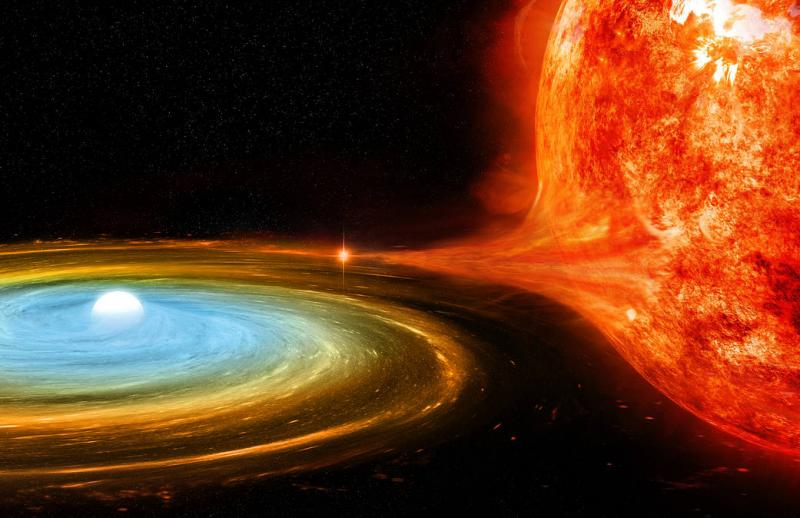
\includegraphics[width=0.6\linewidth]{x-ray-burst.jpg}
%         \caption{Low mass neutron star binaries: Neutron Star accreting mass from its main sequence companion star due to Roche Lobe Overflow. [JINA WEB]}
%     \end{figure}
    
% \end{frame}

% \begin{frame}
%     \frametitle{Motivation}
    
%     \begin{block}{Why?}
%         \large What is the motivation behind flame propagation simulations for X-ray bursts? Why is it important?
%     \end{block}
    
%     \begin{itemize}
%         \item Accretion timescale: $\sim 10^4$ s vs. burst timescale: $\sim 5$ s.
%         \item Burst Oscillation Behavior
%     \end{itemize}
% \end{frame}


\begin{frame}
    \frametitle{Introduction}
        \begin{block}{Goals}
            \begin{itemize}
                \item Study the dynamics of the propagating He flames in X-ray bursts via numerical simulation.
                \item Study the effects of various reaction networks.
            \end{itemize}
        \end{block}

        \begin{columns}
            \column{0.7\linewidth}
            \begin{figure}
                \centering
                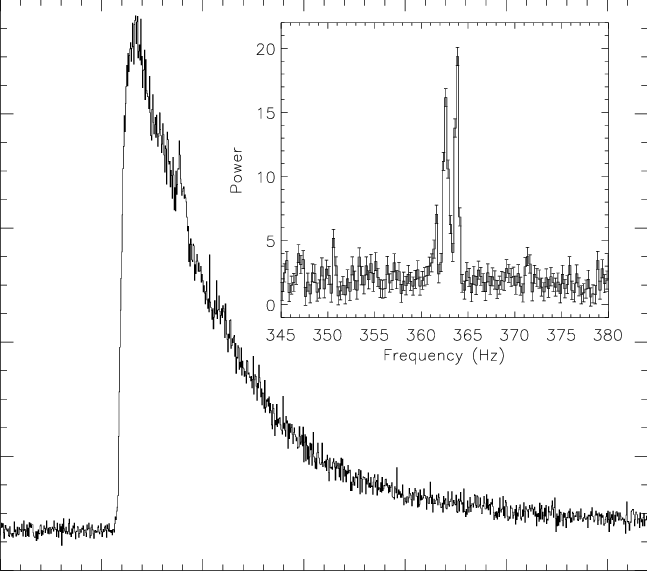
\includegraphics[width=0.68\linewidth]{x-ray-burst-lightcurve.png}
                % \caption{\scriptsize An X-ray burst light curve from 4U 1728–34 showing burst oscillation behavior. \cite{strohmayer_2009}}
            \end{figure}

            \column{0.3\linewidth}
            {\color{blue}Figure:} An X-ray burst light curve from 4U 1728–34 showing burst oscillation behavior. \cite{strohmayer_2009}
        \end{columns}



  
\end{frame}

\section{Nuclear Reaction Networks}

% \begin{frame}{Networks}
%     \begin{center}
%         \Huge {\it Effects of different networks}
%     \end{center}
% \end{frame}

\subsection{Overview of reaction networks}


\begin{frame}
\frametitle{Network: {\tt aprox13}}
    % \begin{columns}
    %     \column{0.7\linewidth}
    %         \begin{figure}
    %             \centering
    %             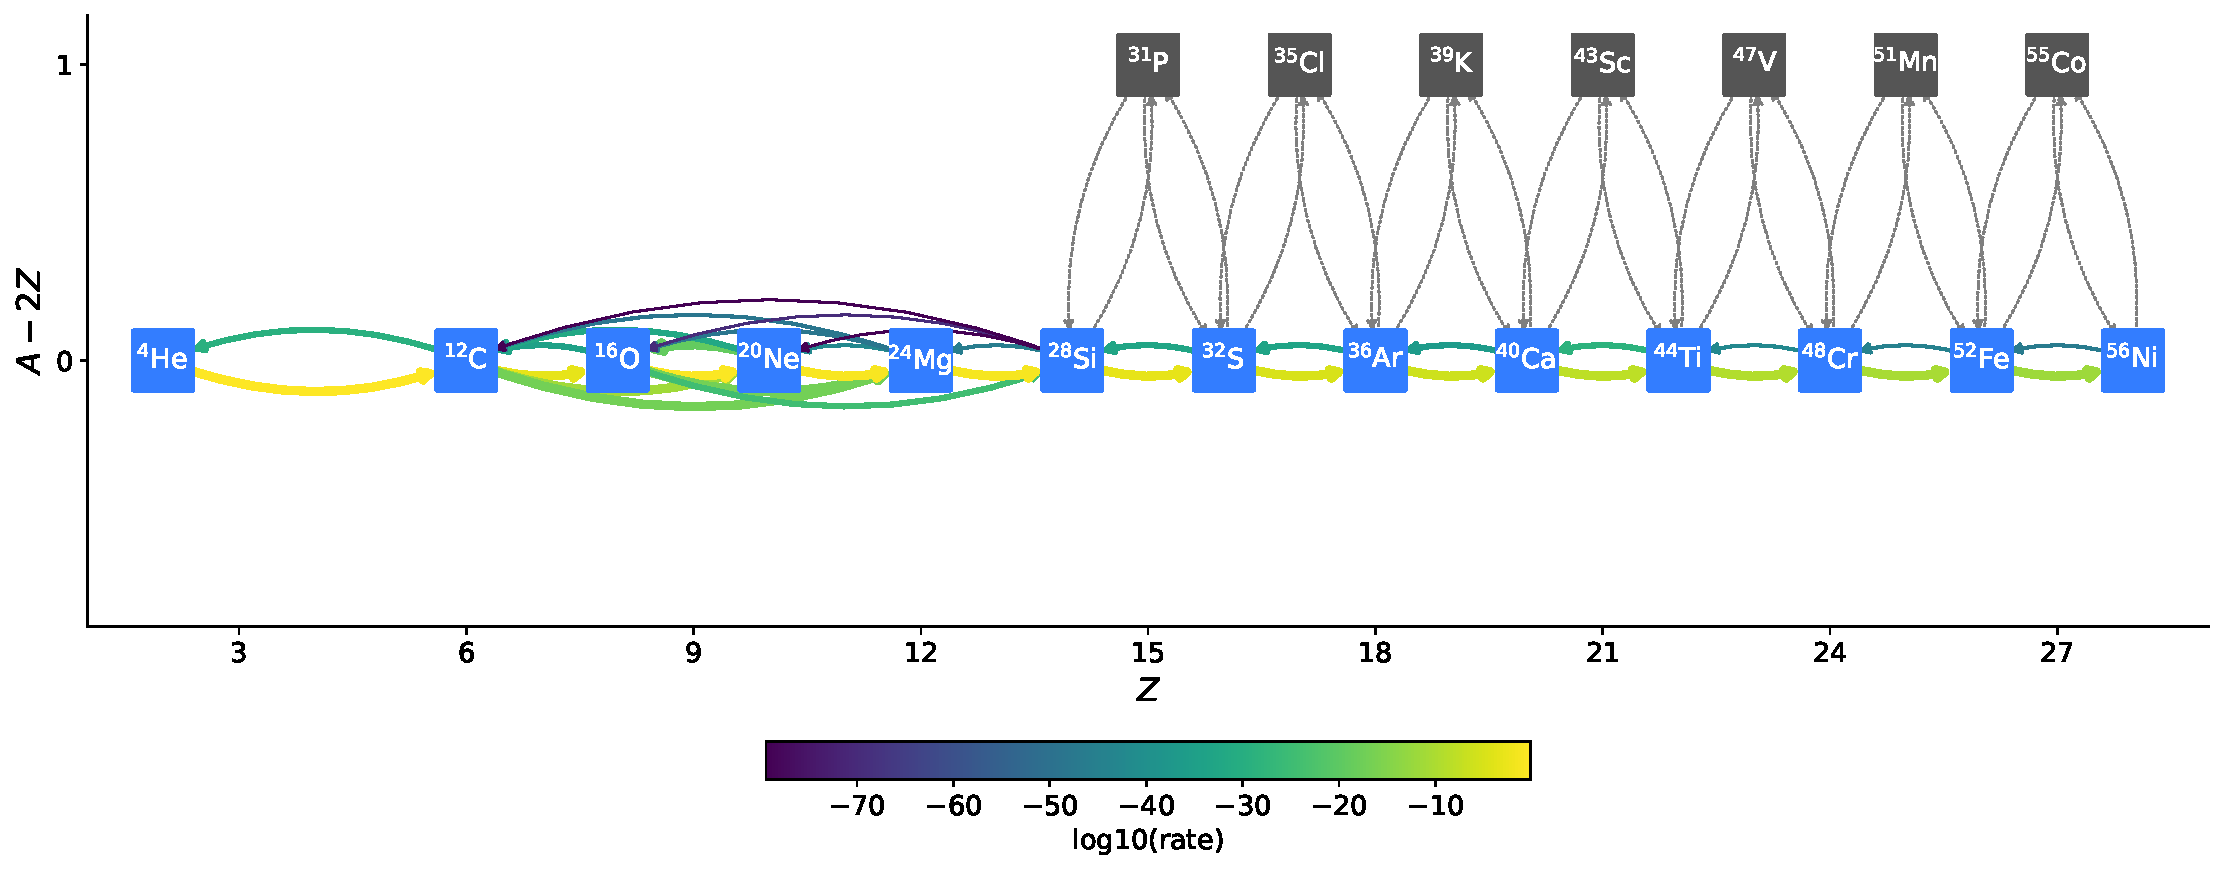
\includegraphics[width=1\linewidth]{aprox13.pdf}
    %         \end{figure}
        
    %     \column{0.3\linewidth}
    %         Figure: Overview of {\tt aprox13}, rates are integrated with $\rho = 10^6$ g $\mathrm{cm}^{-3}$ and $T = 2.0 \times 10^9$ K.
    % \end{columns}
    \begin{figure}
        \centering
        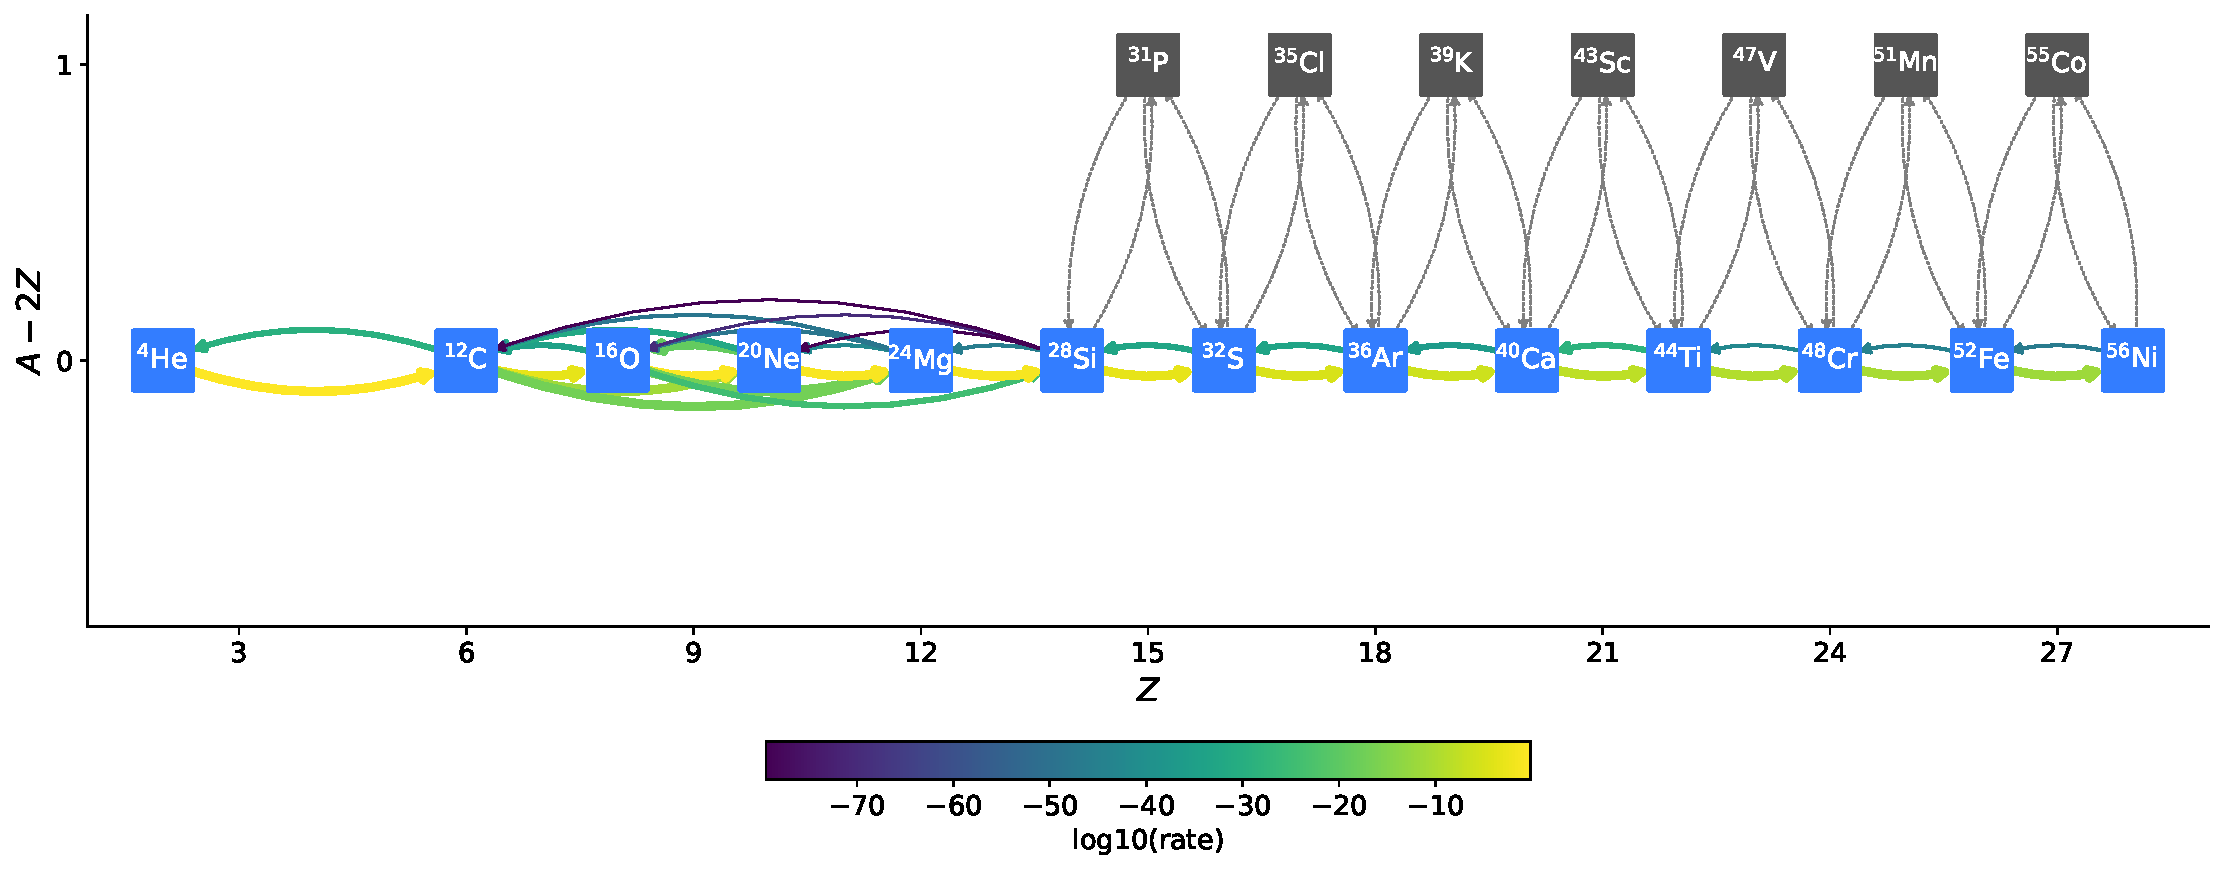
\includegraphics[width=1\linewidth]{aprox13.pdf}
        \caption{\scriptsize Overview of {\tt aprox13}, rates with condition: $\rho = 10^6$ g $\mathrm{cm}^{-3}$ and $T = 2.0 \times 10^9$ K. Generated using {\sf pynucastro}: \url {https://github.com/pynucastro/pynucastro}}
    \end{figure}
    \begin{block}{Feature}
        \begin{itemize}
            \item $(\alpha, \mbox{p})(\mbox{p}, \gamma)$ approximation
            \item 13 isotopes, 31 rates
        \end{itemize}
    \end{block}

\end{frame}


\begin{frame}
\frametitle{Network: {\tt subch full}}
    \begin{figure}
        \centering
        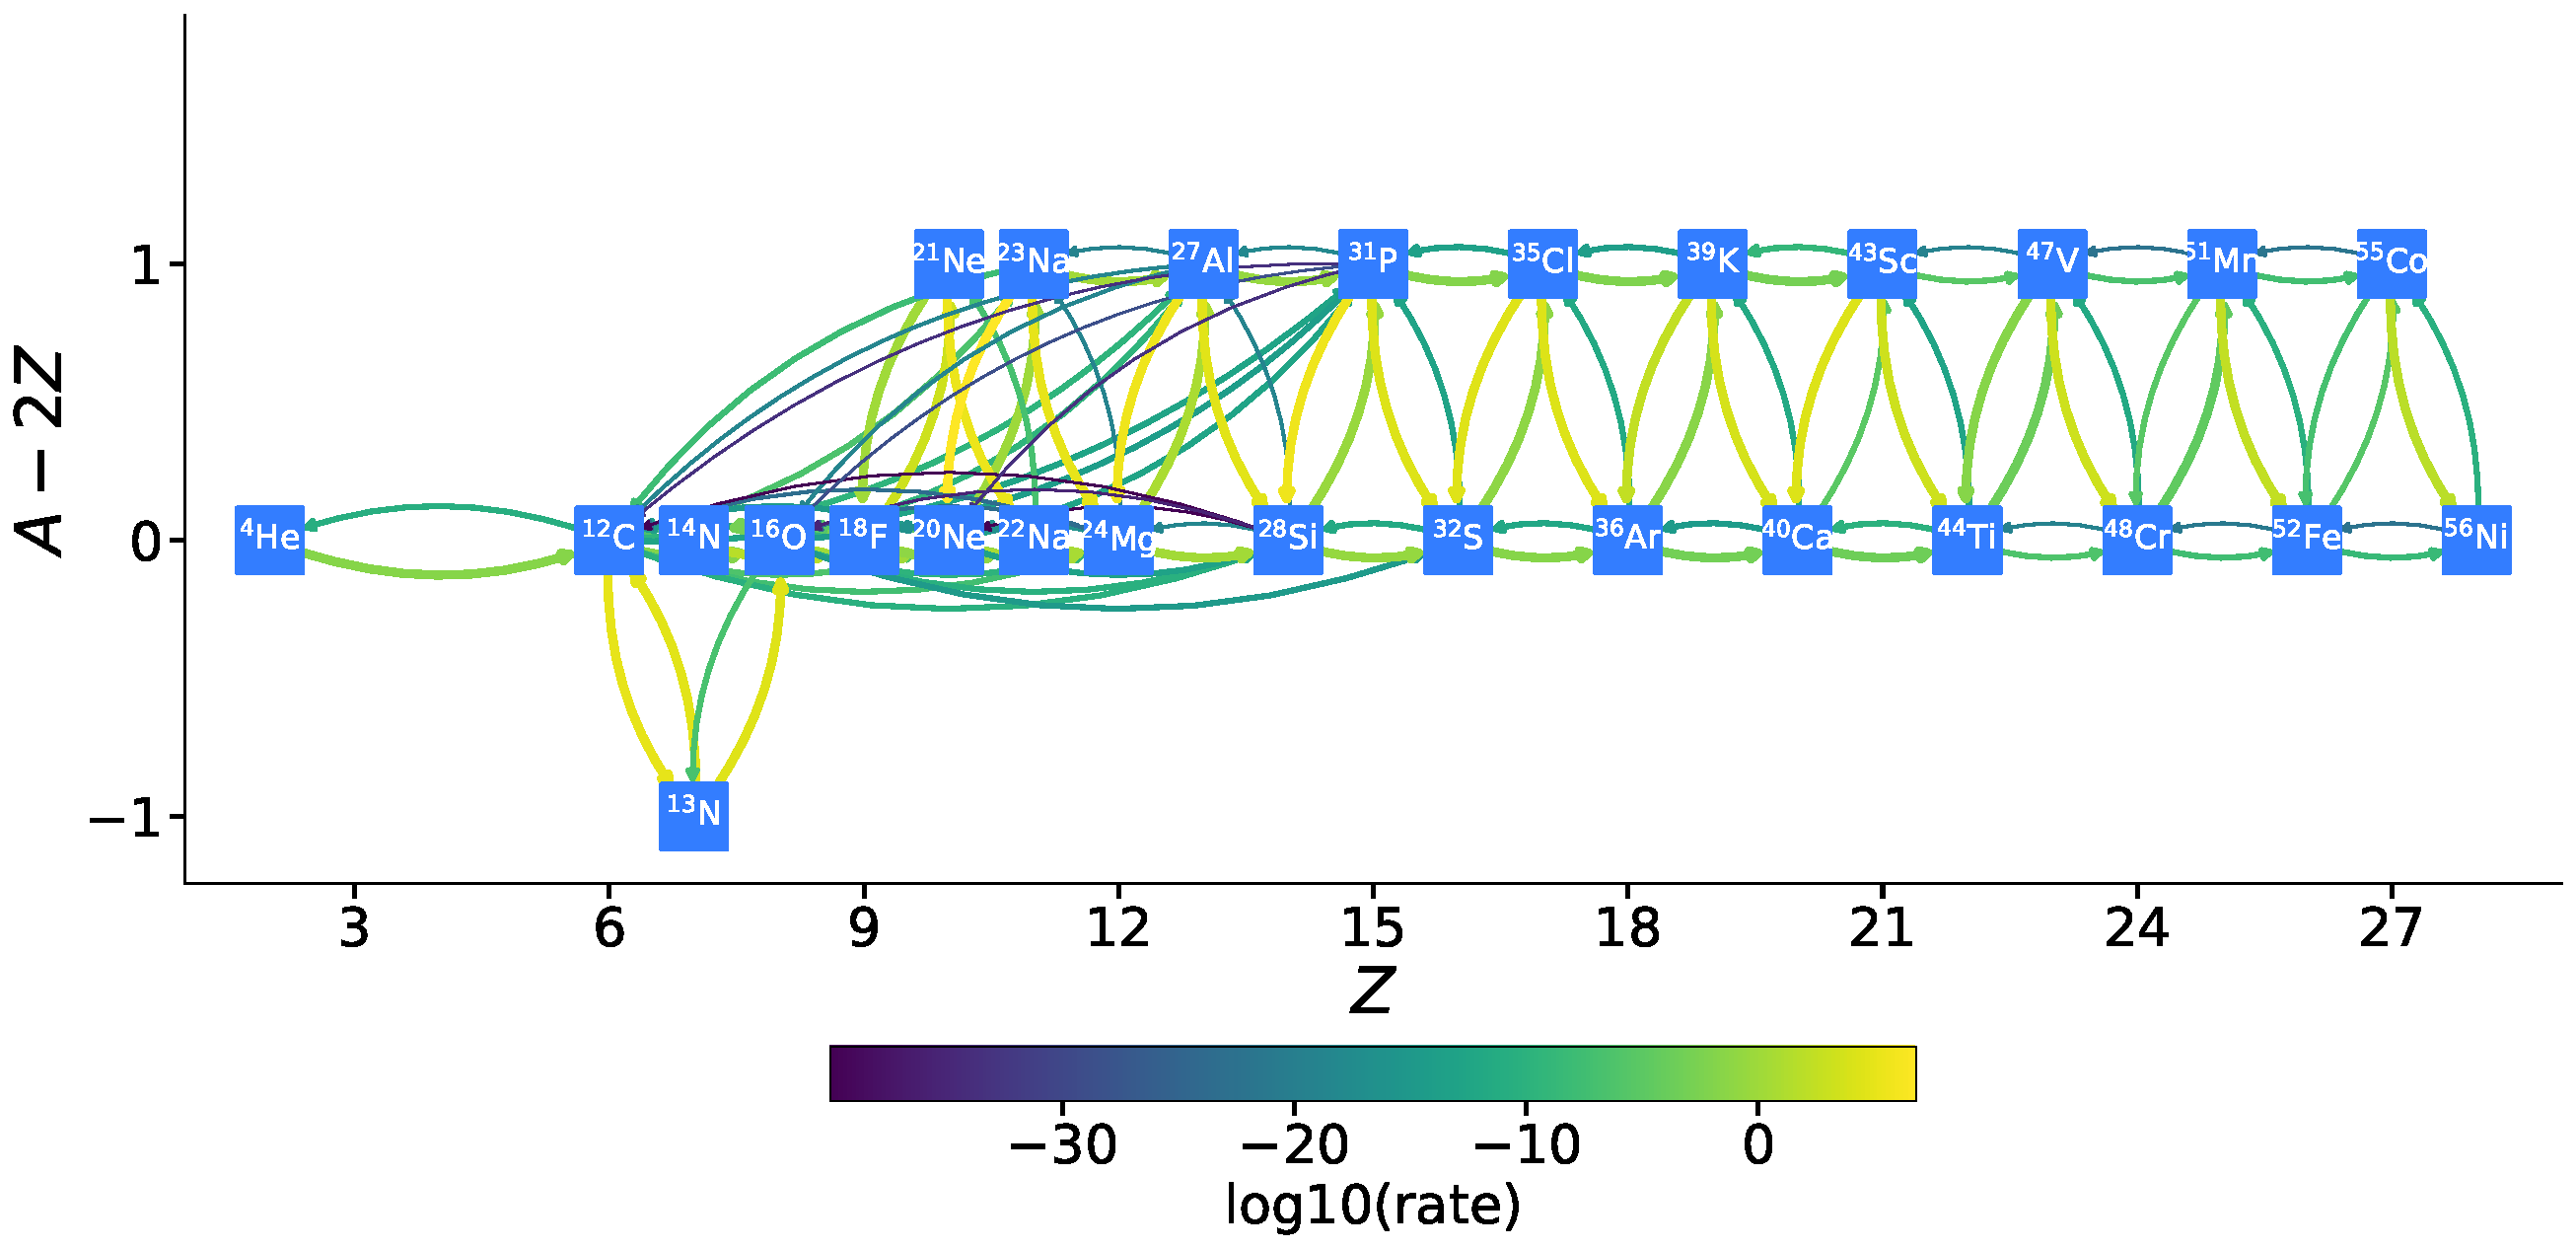
\includegraphics[width=1\linewidth]{subch_full.pdf}
        \caption{\scriptsize Overview of {\tt subch full}, rates with condition $\rho = 10^6$ g $\mathrm{cm}^{-3}$ and $T = 2.0 \times 10^9$ K. Generated using {\sf pynucastro}: \url {https://github.com/pynucastro/pynucastro}}
    \end{figure}

    \begin{block}{Feature}
        \begin{itemize}
            \item \scriptsize No $(\alpha, \mbox{p})(\mbox{p}, \gamma)$ approximation
            \item \scriptsize Additional rates, such as ${}^{12}\mbox{C} ({}^{12}\mbox{C}, p){}^{23}\mbox{Na}$ to give complete representation on carbon and oxygen burning.
            \item \scriptsize Additional rates, ${}^{14}\mbox{N}(\alpha,\gamma){}^{18}\mbox{F}(\alpha, \mbox{p}){}^{21}\mbox{Ne}$ and ${}^{12}\mbox{C}(\mbox{p}, \gamma) {}^{13}\mbox{N}(\alpha, \mbox{p}){}^{16}\mbox{O}$, discussed in Shen \& Bildsten 2009 and Weinberg 2006 \cite{Shen_2009,Weinberg_2006}.
            \item 28 isotopes, 107 rates
        \end{itemize}
    \end{block}
\end{frame}

\begin{frame}
\frametitle{Network: {\tt subch full mod}}
    \begin{figure}
        \centering
        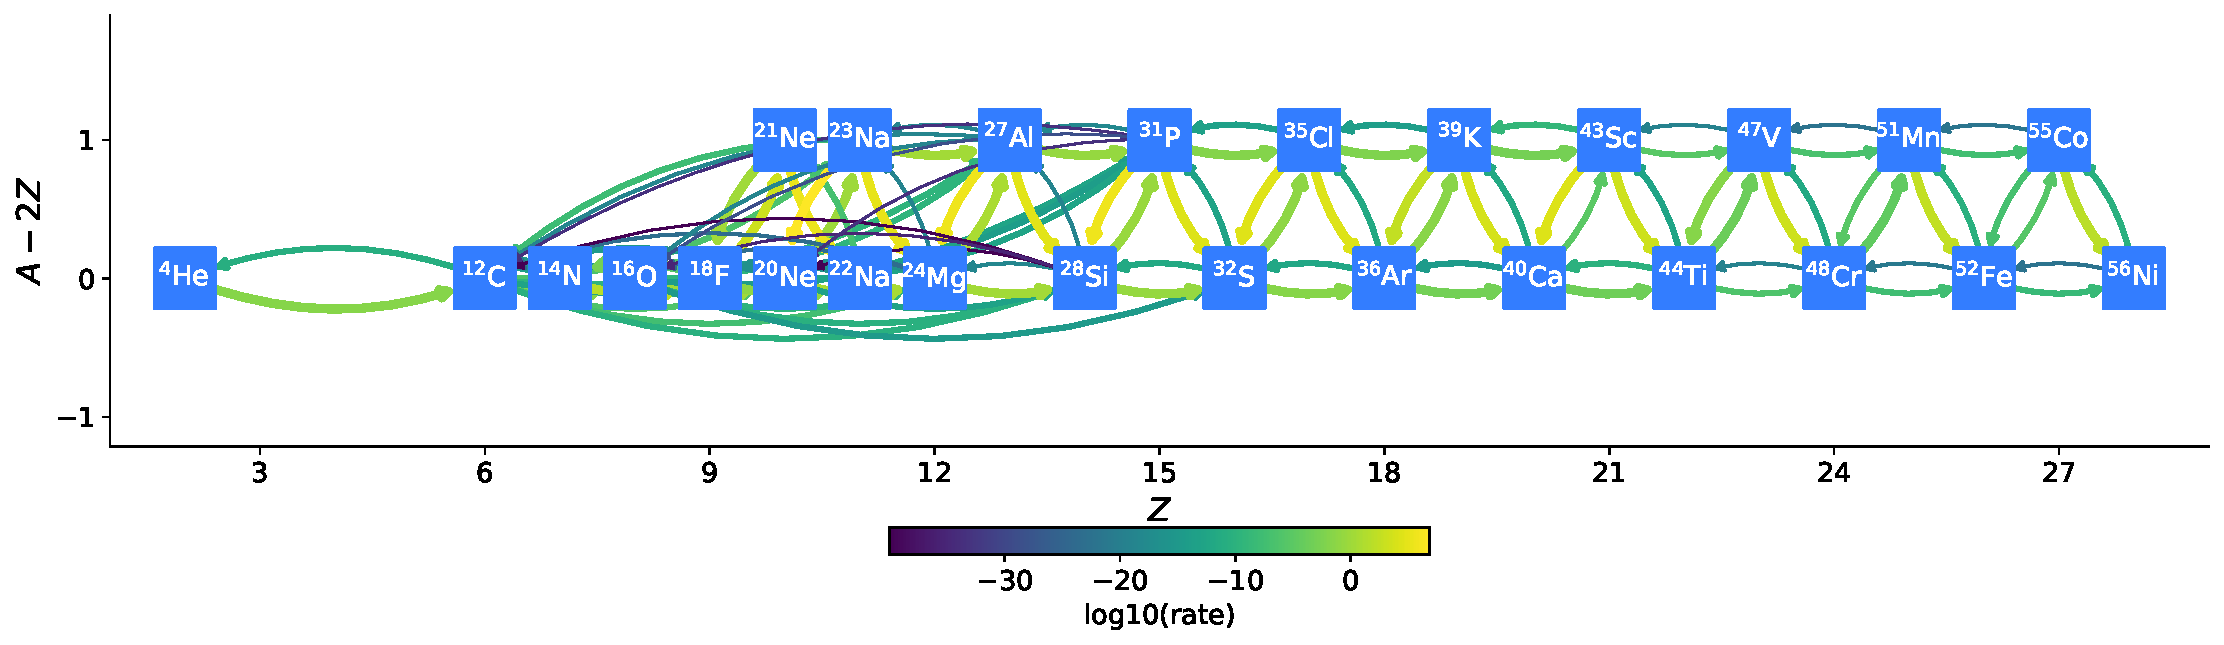
\includegraphics[width=1\linewidth]{subch_full_mod.pdf}
        \caption{Overview of {\tt subch full mod}, rates with condition $\rho = 10^6$ g $\mathrm{cm}^{-3}$ and $T = 2.0 \times 10^9$ K. Generated using {\sf pynucastro}: \url {https://github.com/pynucastro/pynucastro}}
    \end{figure}
    \begin{block}{Feature}
        \begin{itemize}
            \item Identical to {\tt subch full} but ${}^{12}\mbox{C}(\mbox{p}, \gamma) {}^{13}\mbox{N}(\alpha, \mbox{p}){}^{16}\mbox{O}$ and its reverse rate are disabled.
            \item 27 isotopes, 103 rates
        \end{itemize}
    \end{block}
\end{frame}


\begin{frame}
\frametitle{Network: {\tt subch simple}}
\begin{figure}
    \centering
    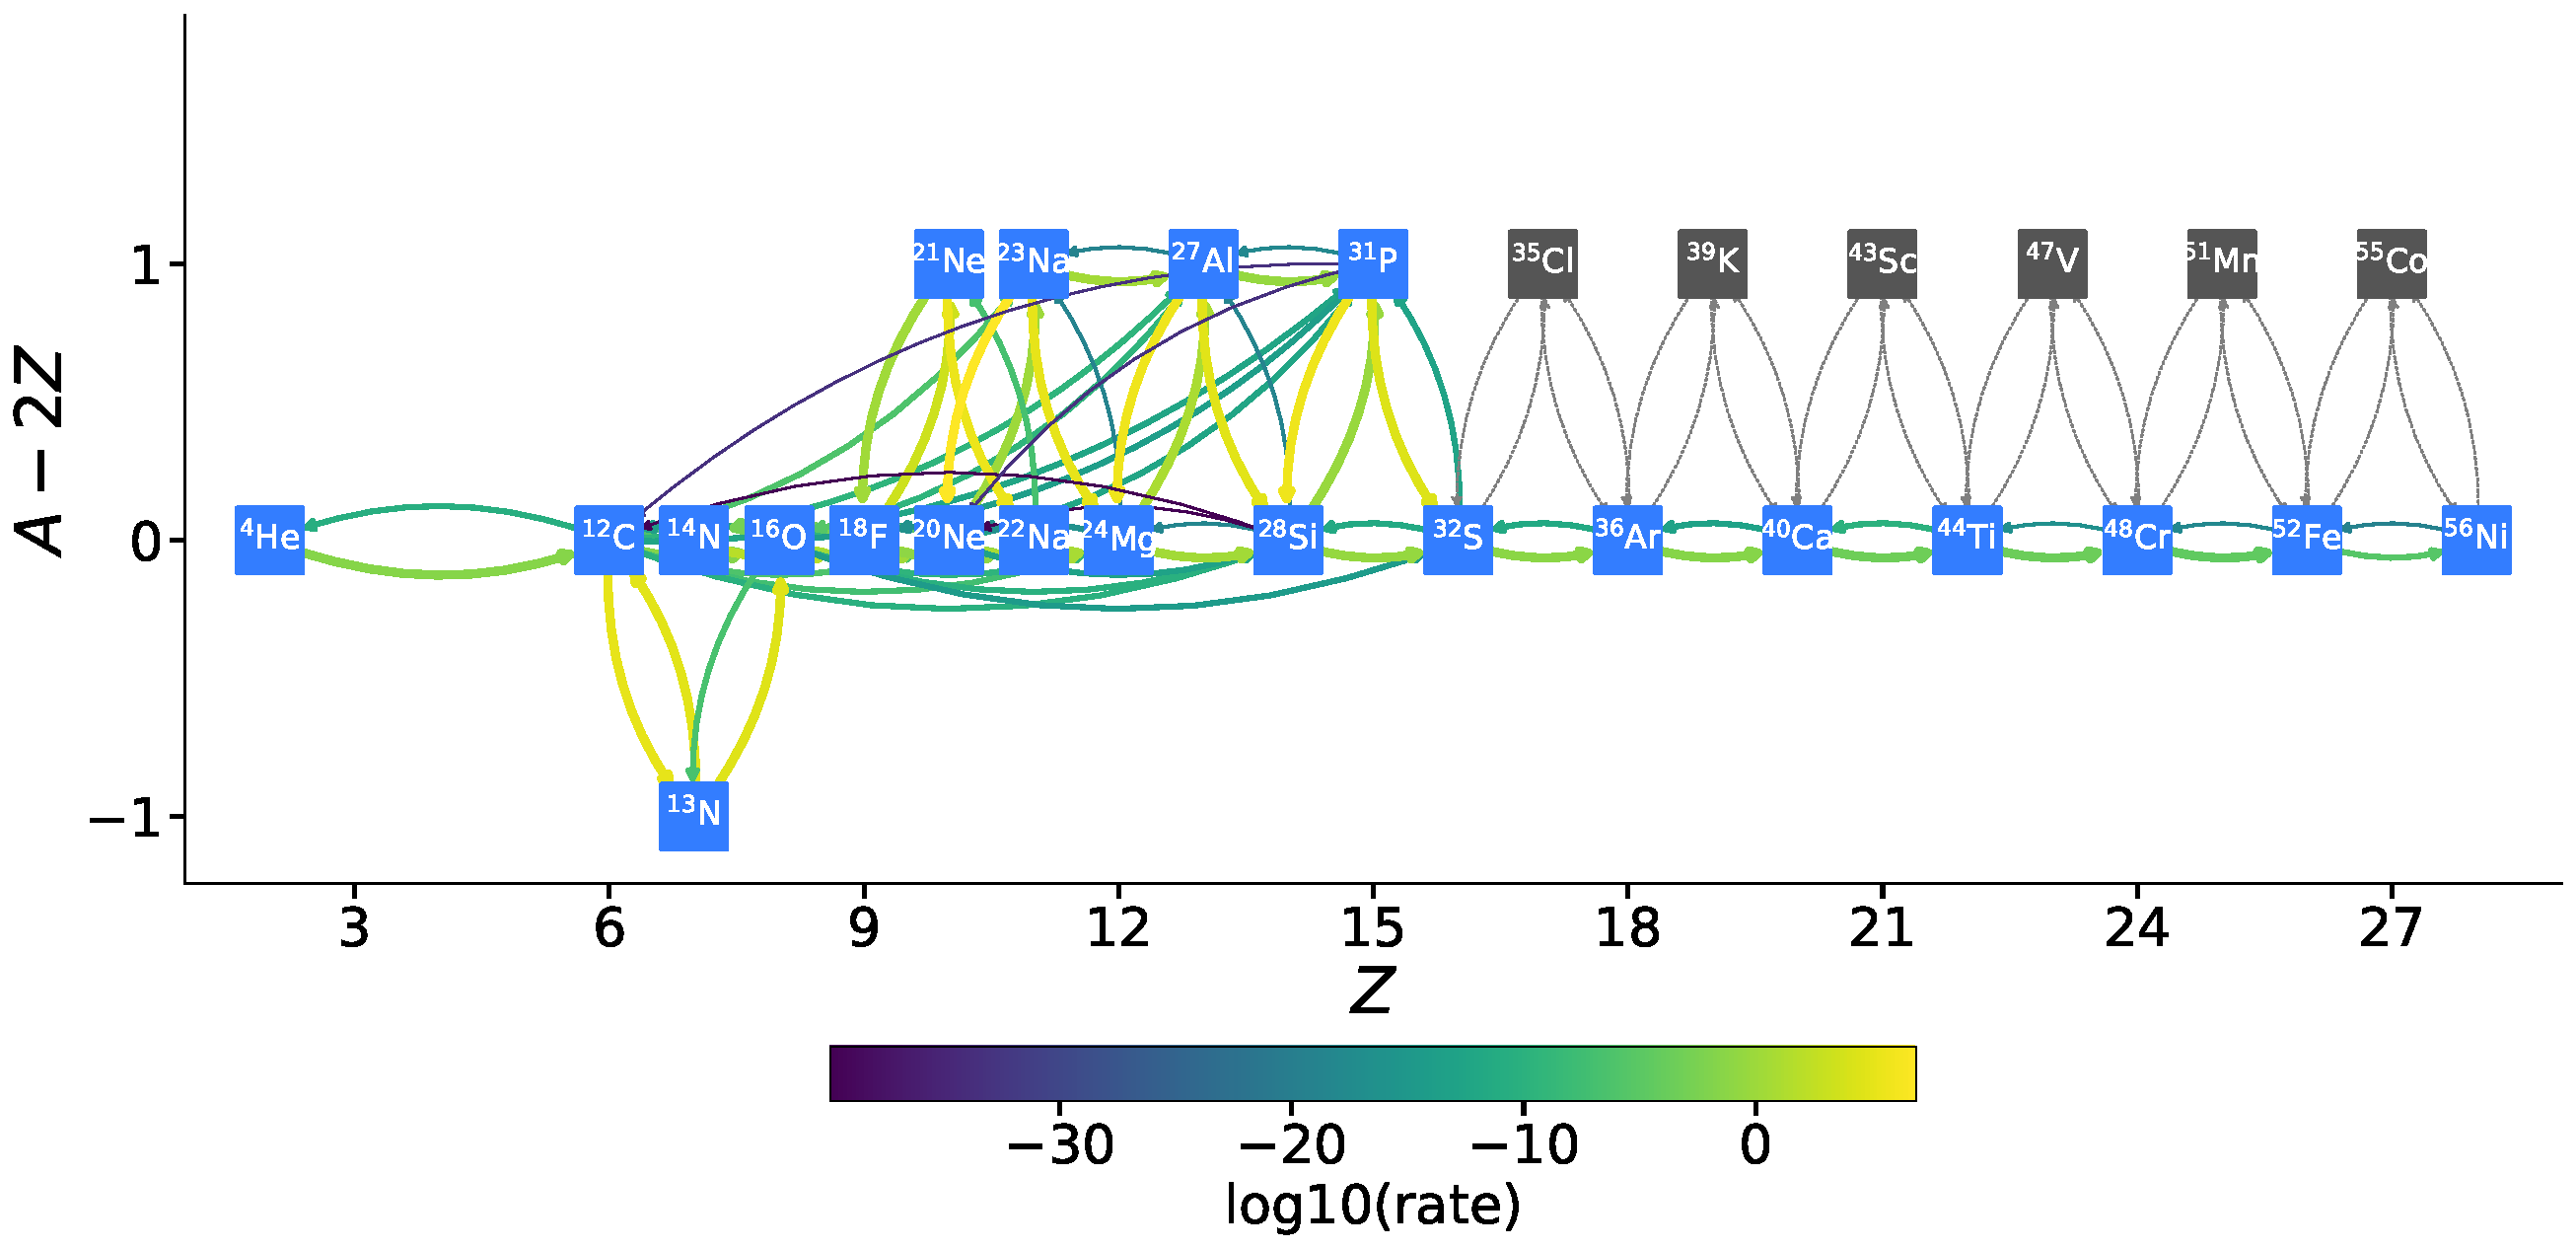
\includegraphics[width=1\linewidth]{subch_simple.pdf}
    \caption{\scriptsize Overview of {\tt subch simple}, rates with condition $\rho = 10^6$ g $\mathrm{cm}^{-3}$ and $T = 2.0 \times 10^9$ K. Generated using {\sf pynucastro}: \url {https://github.com/pynucastro/pynucastro}}
\end{figure}
\begin{block}{Feature}
    \begin{itemize}
        \item \scriptsize $(\alpha, \mbox{p})(\mbox{p}, \gamma)$ approximation for heavy isotopes
        \item \scriptsize The reverse rates of all ${}^{12}\mbox{C} + {}^{12}\mbox{C}$,  ${}^{16}\mbox{O} + {}^{16}\mbox{O}$, and ${}^{16}\mbox{O} + {}^{12}\mbox{C}$ are removed.
        \item \scriptsize Forward and reverse rates of ${}^{12}\mbox{C} + {}^{20}\mbox{Ne}$ , ${}^{23}\mbox{Na}(\alpha, \gamma){}^{27}\mbox{Al}$, and ${}^{27}\mbox{Al}(\alpha, \gamma){}^{31}\mbox{P}$ are removed
        \item 22 isotopes, 57 rates
    \end{itemize}
\end{block}
\end{frame}

% \begin{frame}{Network: Models}
%     % \begin{center}
%     %     \LARGE Plasma Screening
%     % \end{center}
    
%     \begin{table}
%         \resizebox{1\linewidth}{!}{
%         \begin{tabular}{cccc}
%         \toprule
%         Name &
%         Network &
%         Integration &
%         Screening\\ 
%         \midrule
        
%         {\tt aprox13} & {\tt aprox13} & strang-splitting & {\tt SCREEN5} \\
%         {\tt subch full} & {\tt subch full} & strang-splitting & {\tt SCREEN5} \\
%         {\tt subch full mod} & {\tt subch full mod} & strang-splitting & {\tt SCREEN5} \\
%         {\tt subch simple} & {\tt subch simple} & strang-splitting & {\tt SCREEN5} \\
%         % {\tt aprox13 sdc} & {\tt aprox13} & simplified SDC & {\tt SCREEN5} \\
%         % {\tt subch full sdc} & {\tt subch full} & simplified SDC & {\tt SCREEN5} \\
%         % {\tt aprox13 chu} & {\tt aprox13} & strang-splitting & {\tt CHUGUNOV2007} \\
%         \bottomrule
%         \end{tabular}}
%         \caption{This table shows the various settings used for each simulation.}
%     \end{table}
    
% \end{frame}


\section{Numerical Approach}


\begin{frame}
    \frametitle{General Numerical Settings}
    
    \begin{block}{\tt CASTRO}
    An adaptive mesh, astrophysical compressible hydrodynamics simulation code. Freely available at \url{https://github.com/AMReX-Astro/Castro}.
    \end{block}

    \begin{block}{\tt Microphysics}
    Software that contains a collection of microphysics routines such as Equation of State and the RHS of reaction networks. Freely available at \url{https://github.com/AMReX-Astro/Microphysics}.
    \end{block}

    \begin{block}{General Simulation Domain}
        \begin{itemize}
            \item 2-D $r-z$ cylindrical coordinate system assuming azimuthal symmetry.
            \item Corotating Frame
            \item Pure ${}^{4}$He accretion layer
        \end{itemize}
    \end{block}
    
\end{frame}


\subsection{Initial Model}


\begin{frame}
\frametitle{Initial Model}

    \begin{figure}
        \centering
        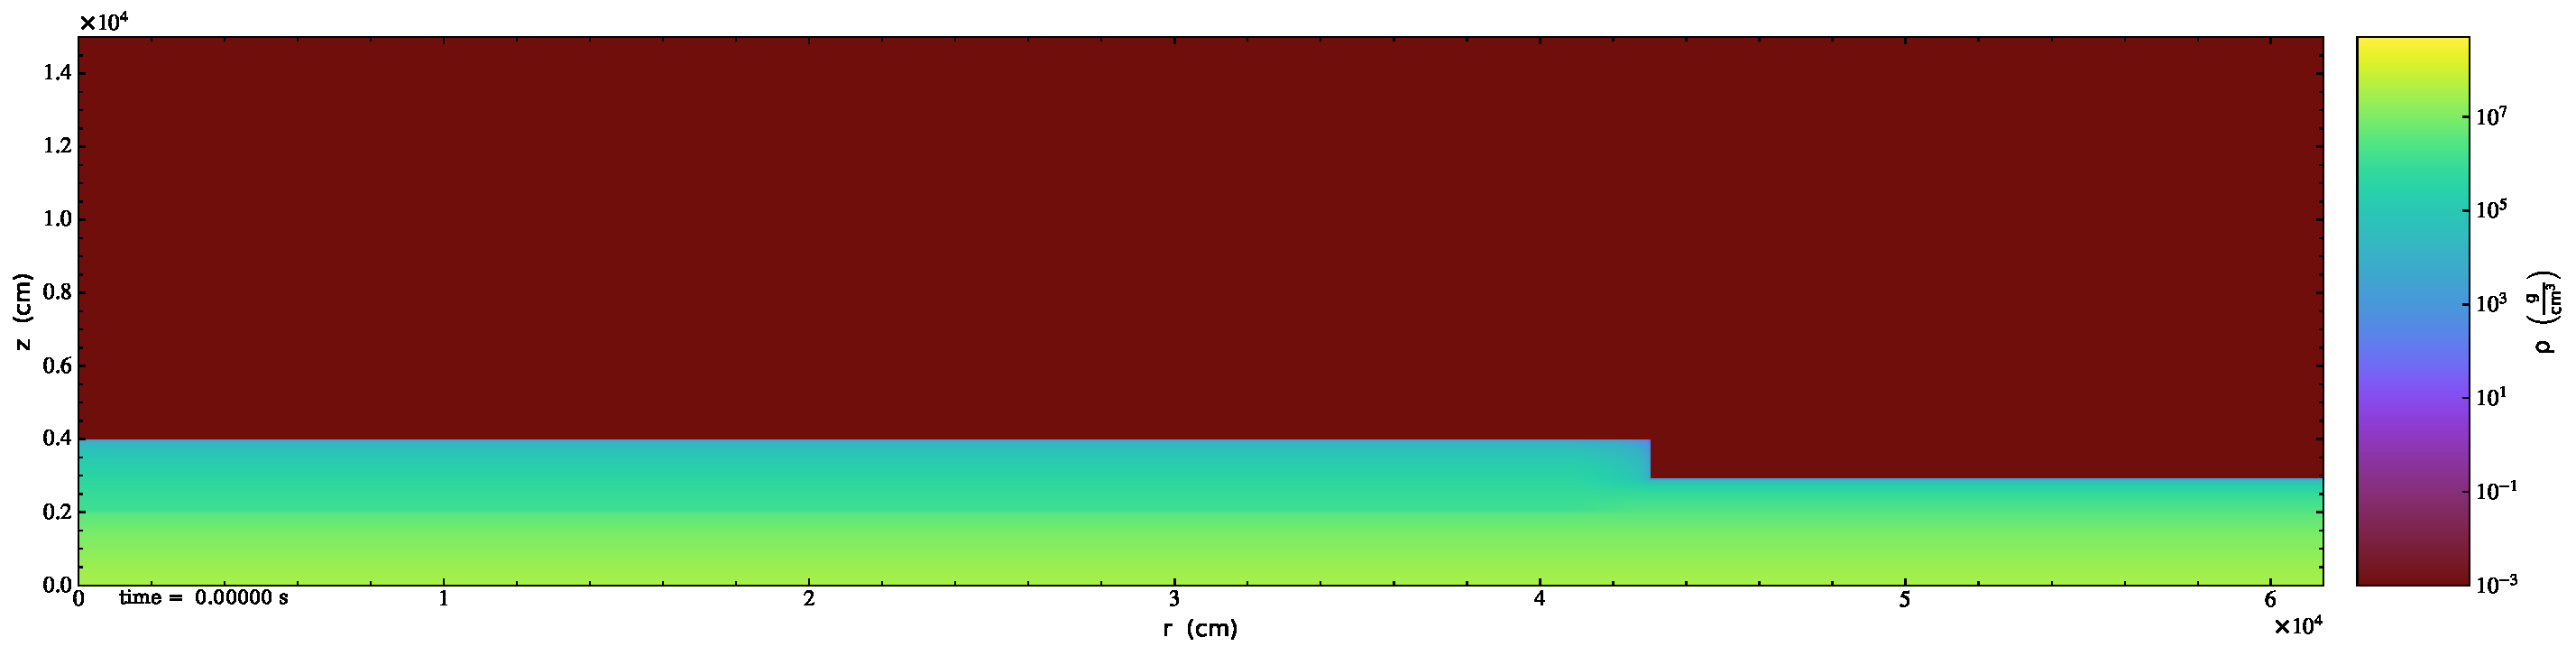
\includegraphics[width=1\linewidth]{init_rho.pdf}
        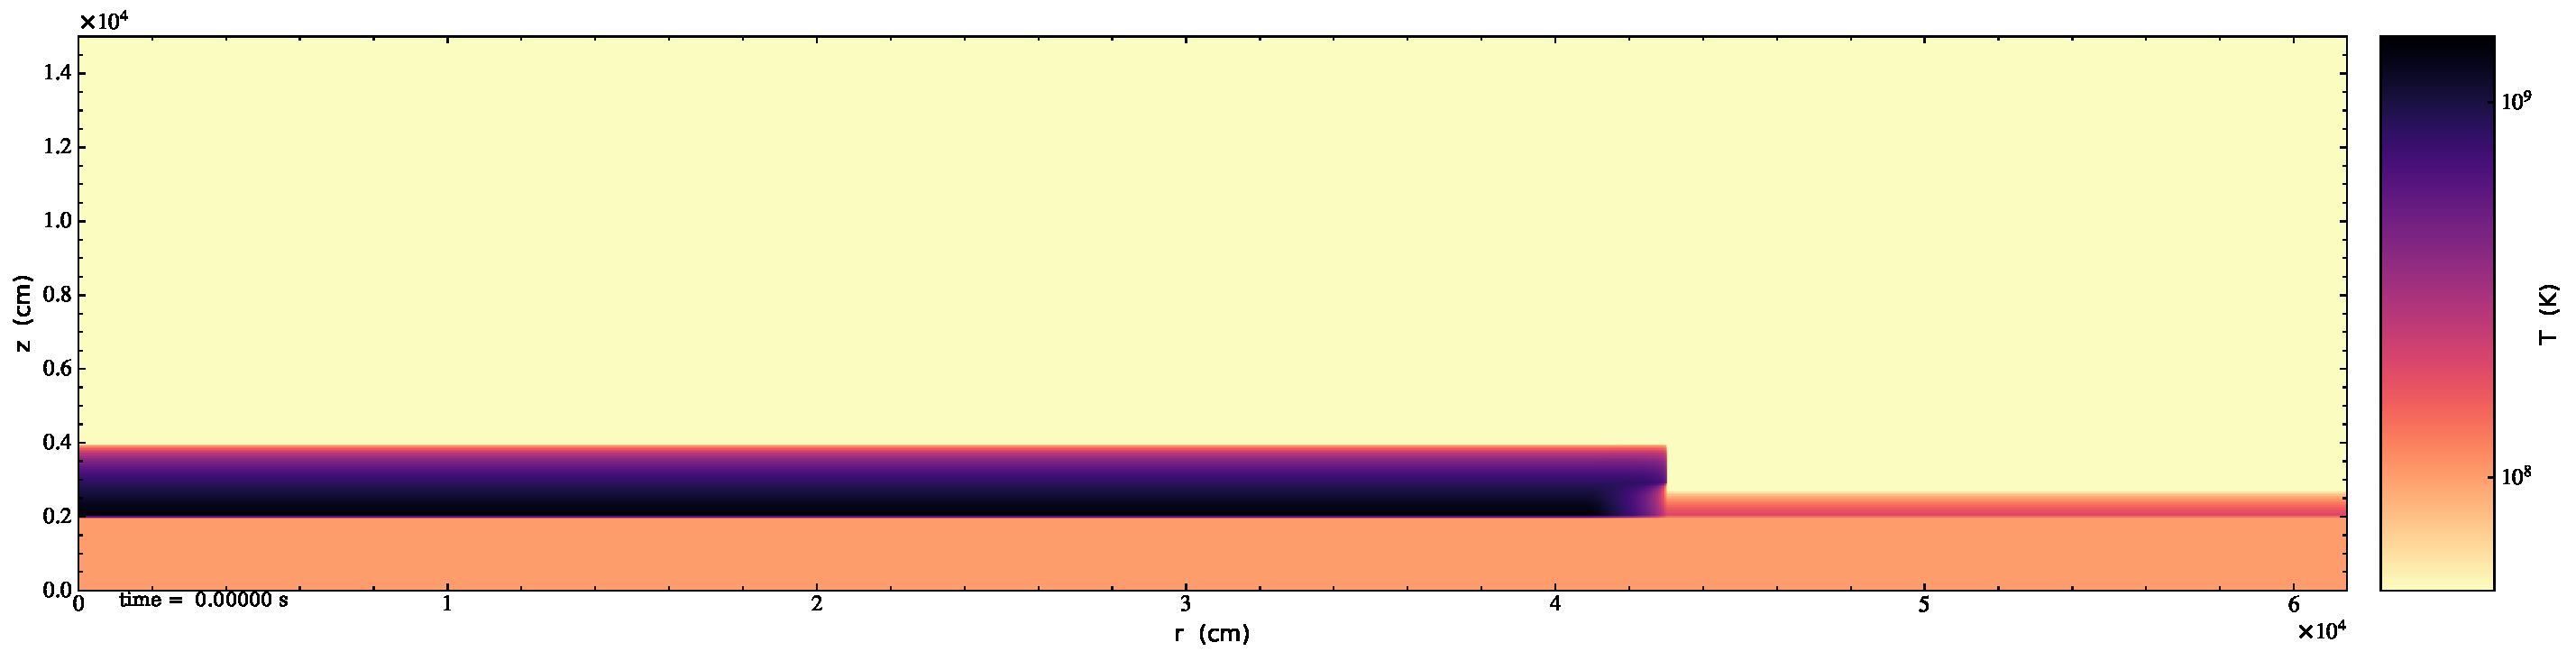
\includegraphics[width=1\linewidth]{init_temp.pdf}
        \caption{Initial temperature and density profile showing 1/3 of the full domain.}
    \end{figure}

\end{frame}



\subsection{Simulation Results}

% \begin{frame}
% \frametitle{Network: $\Bar{A}$ Comparison}
%     \begin{figure}
%         \centering
%         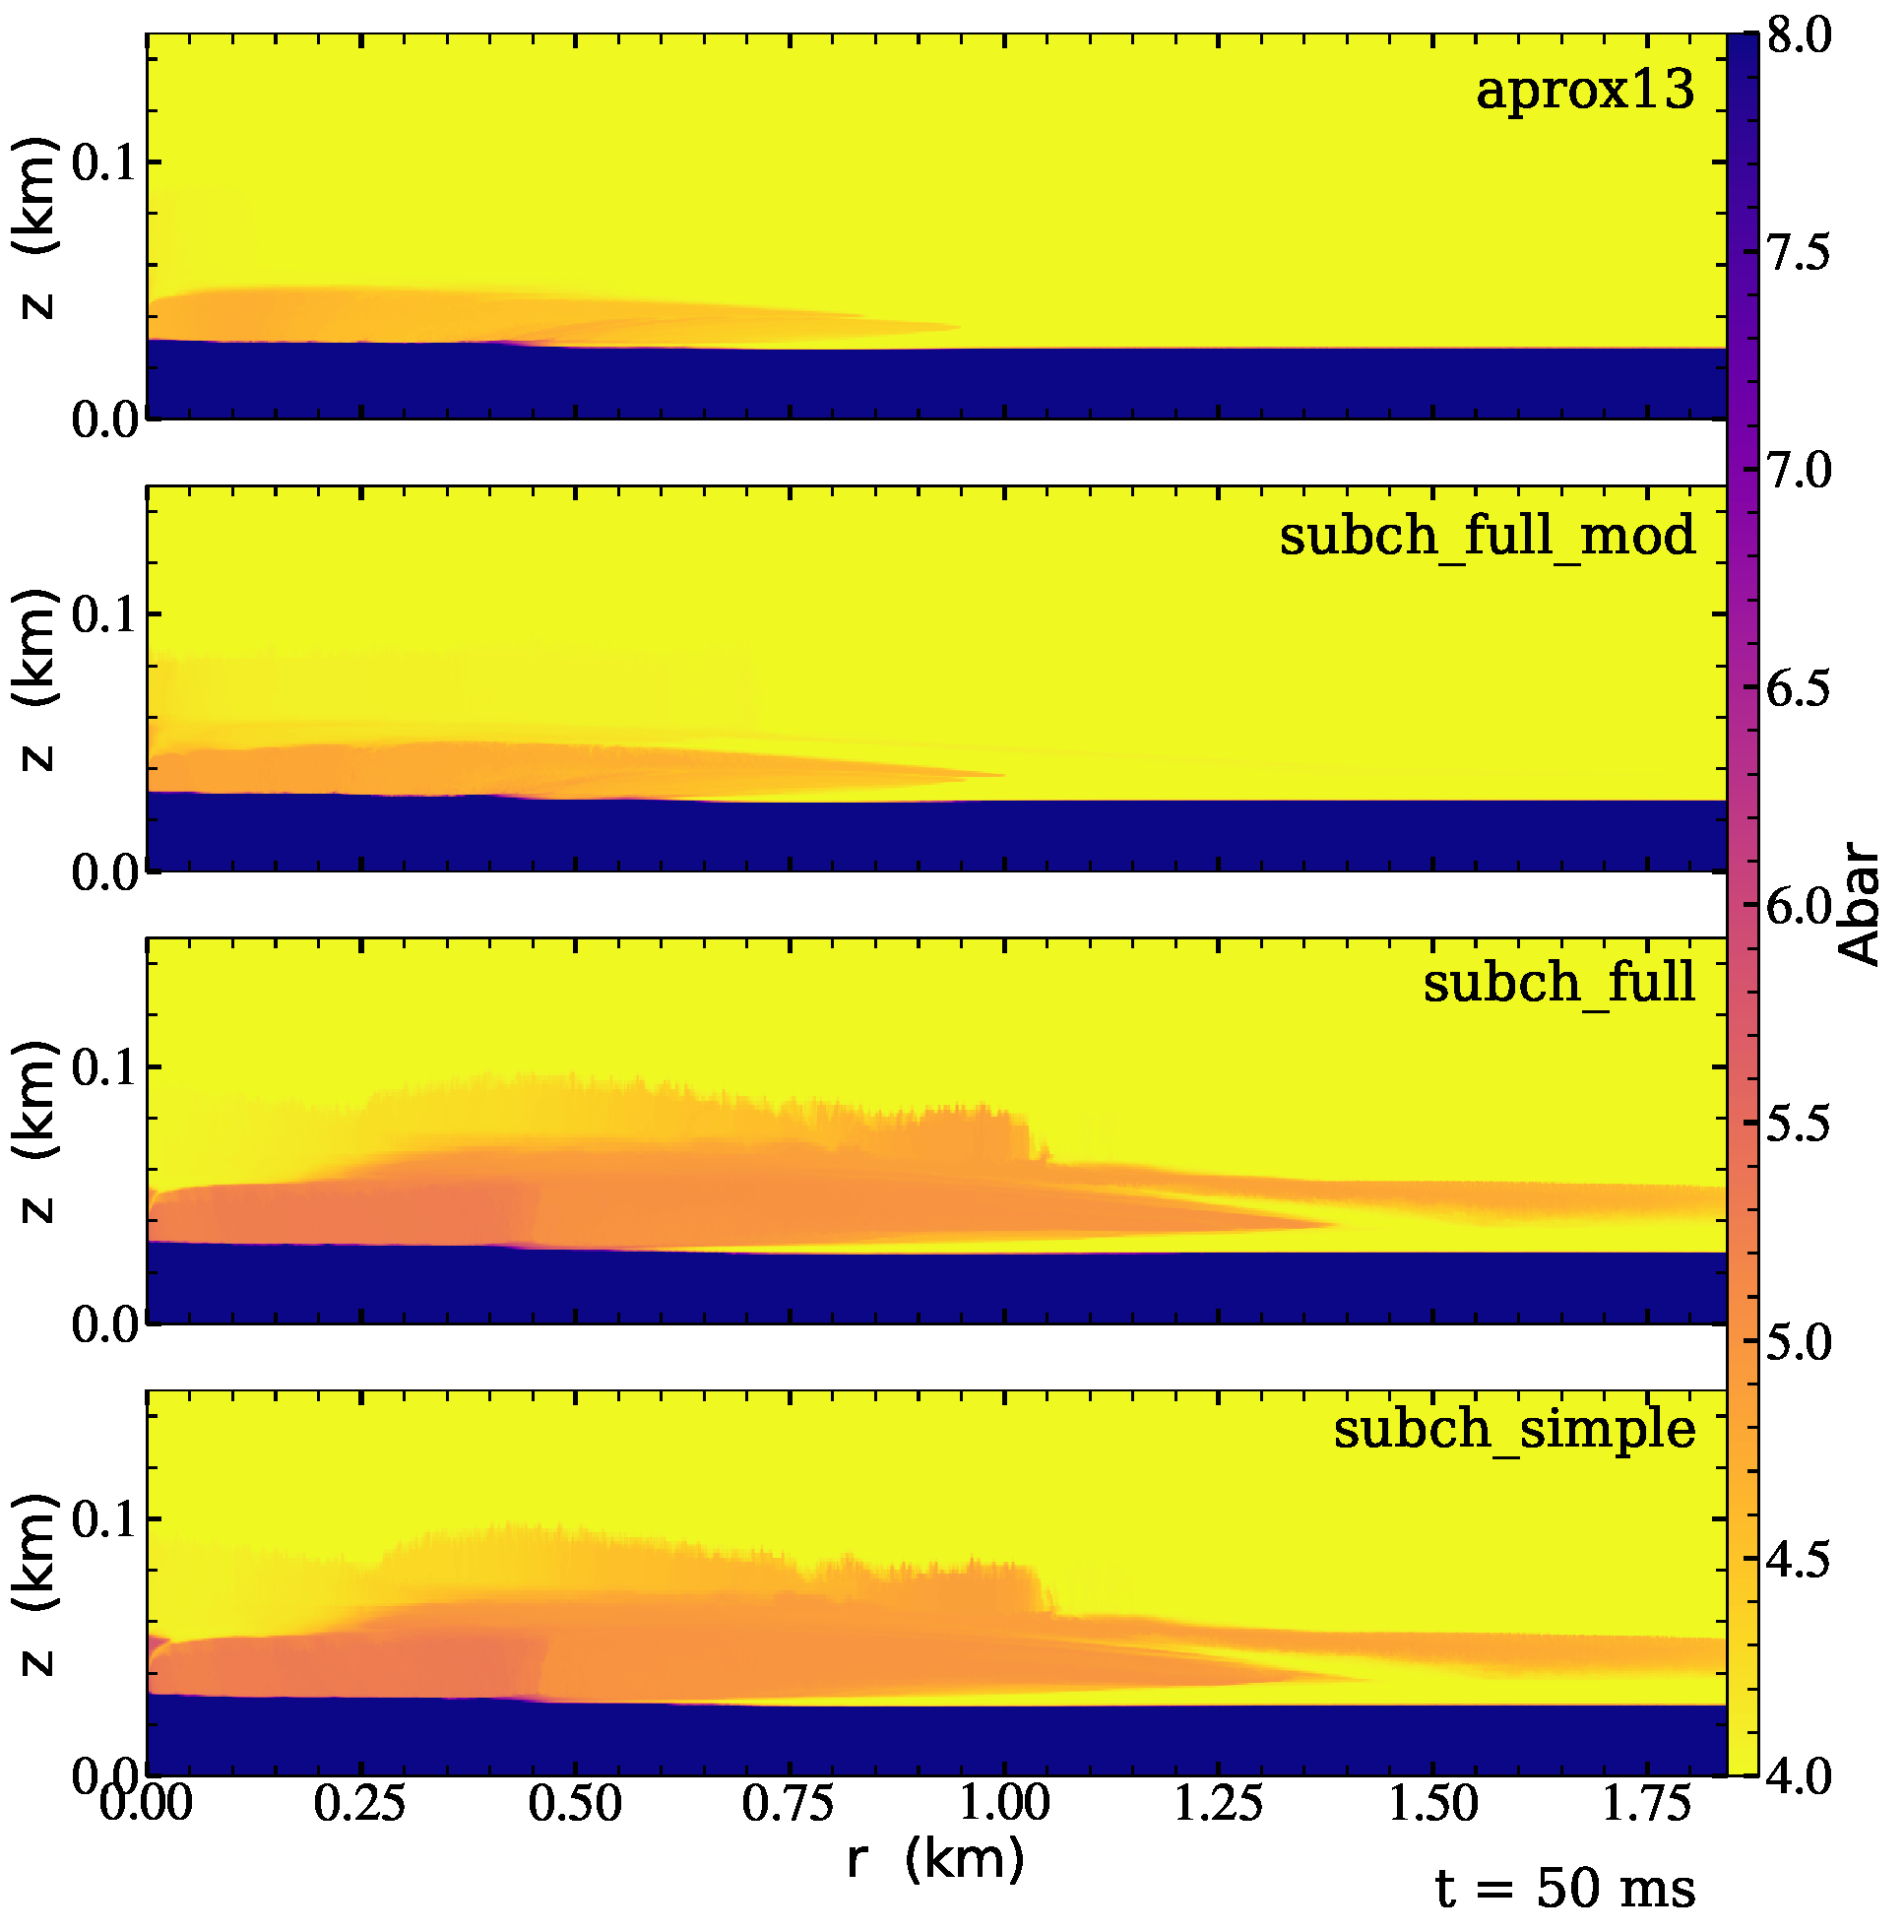
\includegraphics[width=1\linewidth]{network_abar_50ms.pdf}
%         \caption{Slice plots of the flame propagation comparing average atomic weight, $\Bar{A}$, for {\tt aprox13} (top panel), {\tt subch full} (second panel from top), {\tt subch full mod} (third panel), and {\tt subch simple} (last panel) at 50ms.}
%     \end{figure}
% \end{frame}

% \begin{frame}
% \frametitle{Network: $\dot{e}_{nuc}$ Comparison}
%     \begin{figure}
%         \centering
%         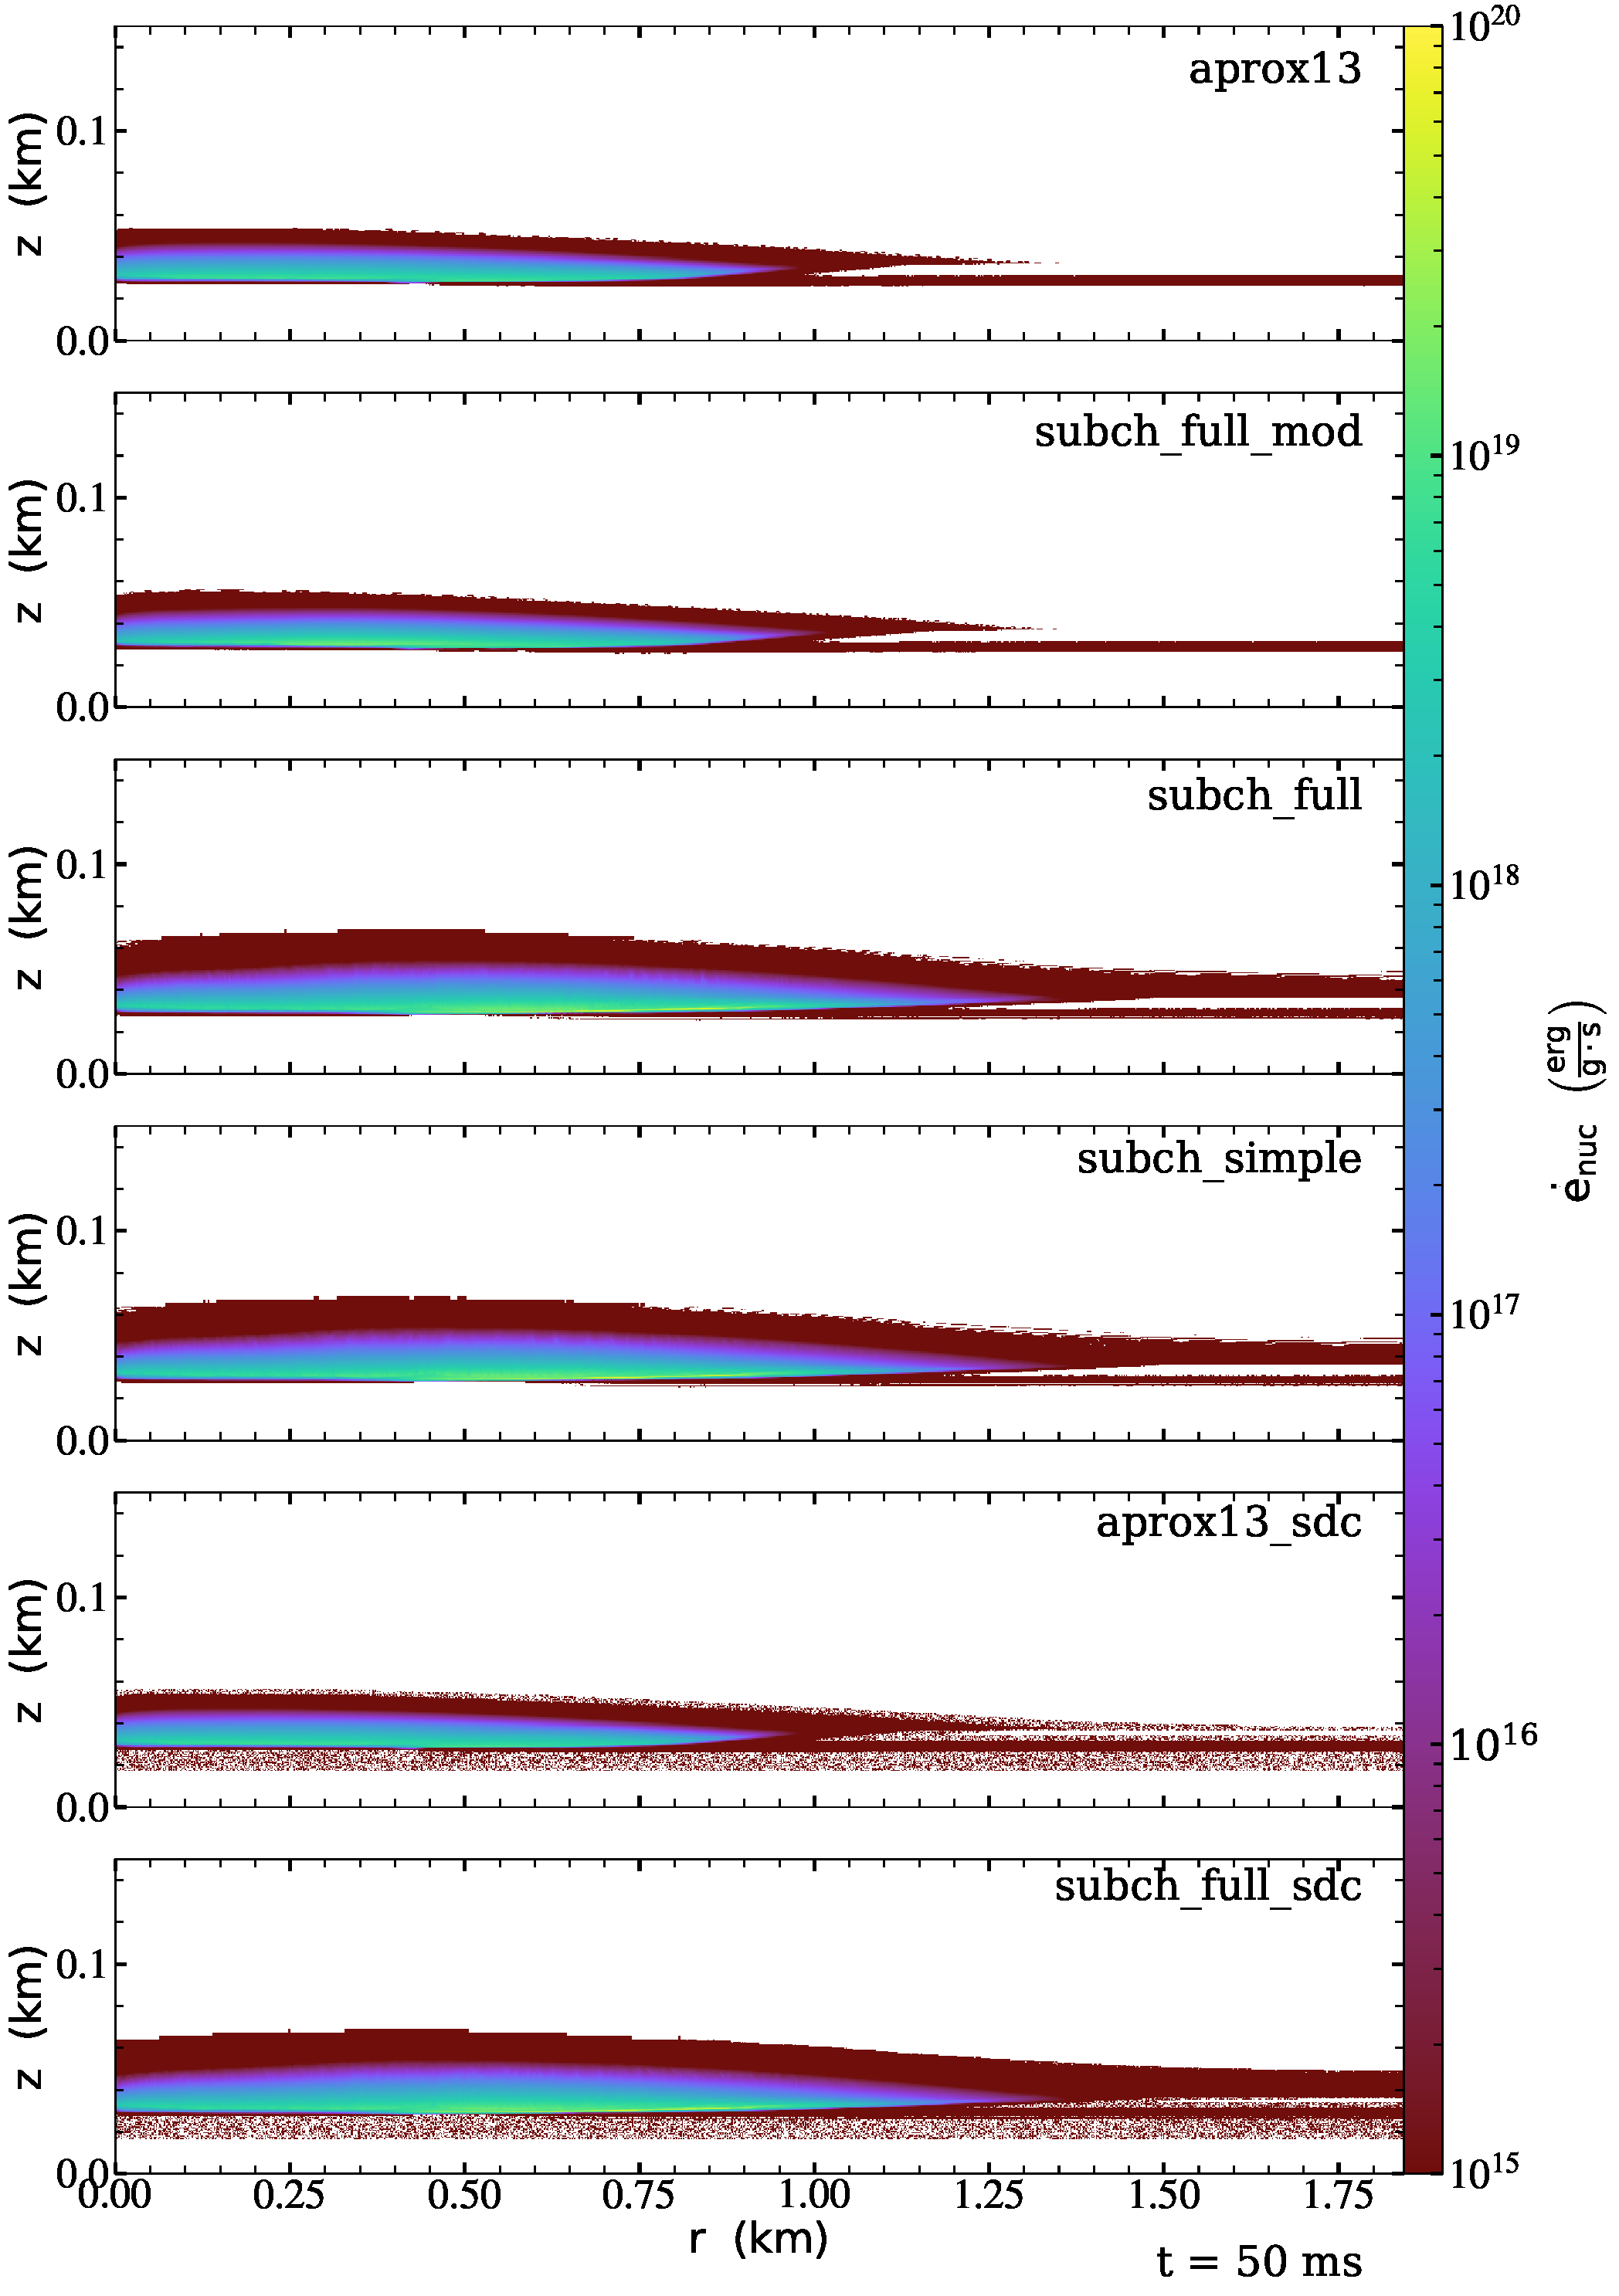
\includegraphics[width=1\linewidth]{network_enuc_50ms.pdf}
%         \caption{This figure shows 4 slice plots of the flame propagation comparing specific energy generation rate, $\dot{e}_{nuc}$, for {\tt aprox13} (top panel), {\tt subch full} (second panel from top), {\tt subch full mod} (third panel), and {\tt subch simple} (last panel) at 50ms.}
%     \end{figure}
% \end{frame}



\begin{frame}
\frametitle{Results: Weighted $T$ and $\dot{e}_{nuc}$ Time Profiles}
    \begin{figure}
        \centering
        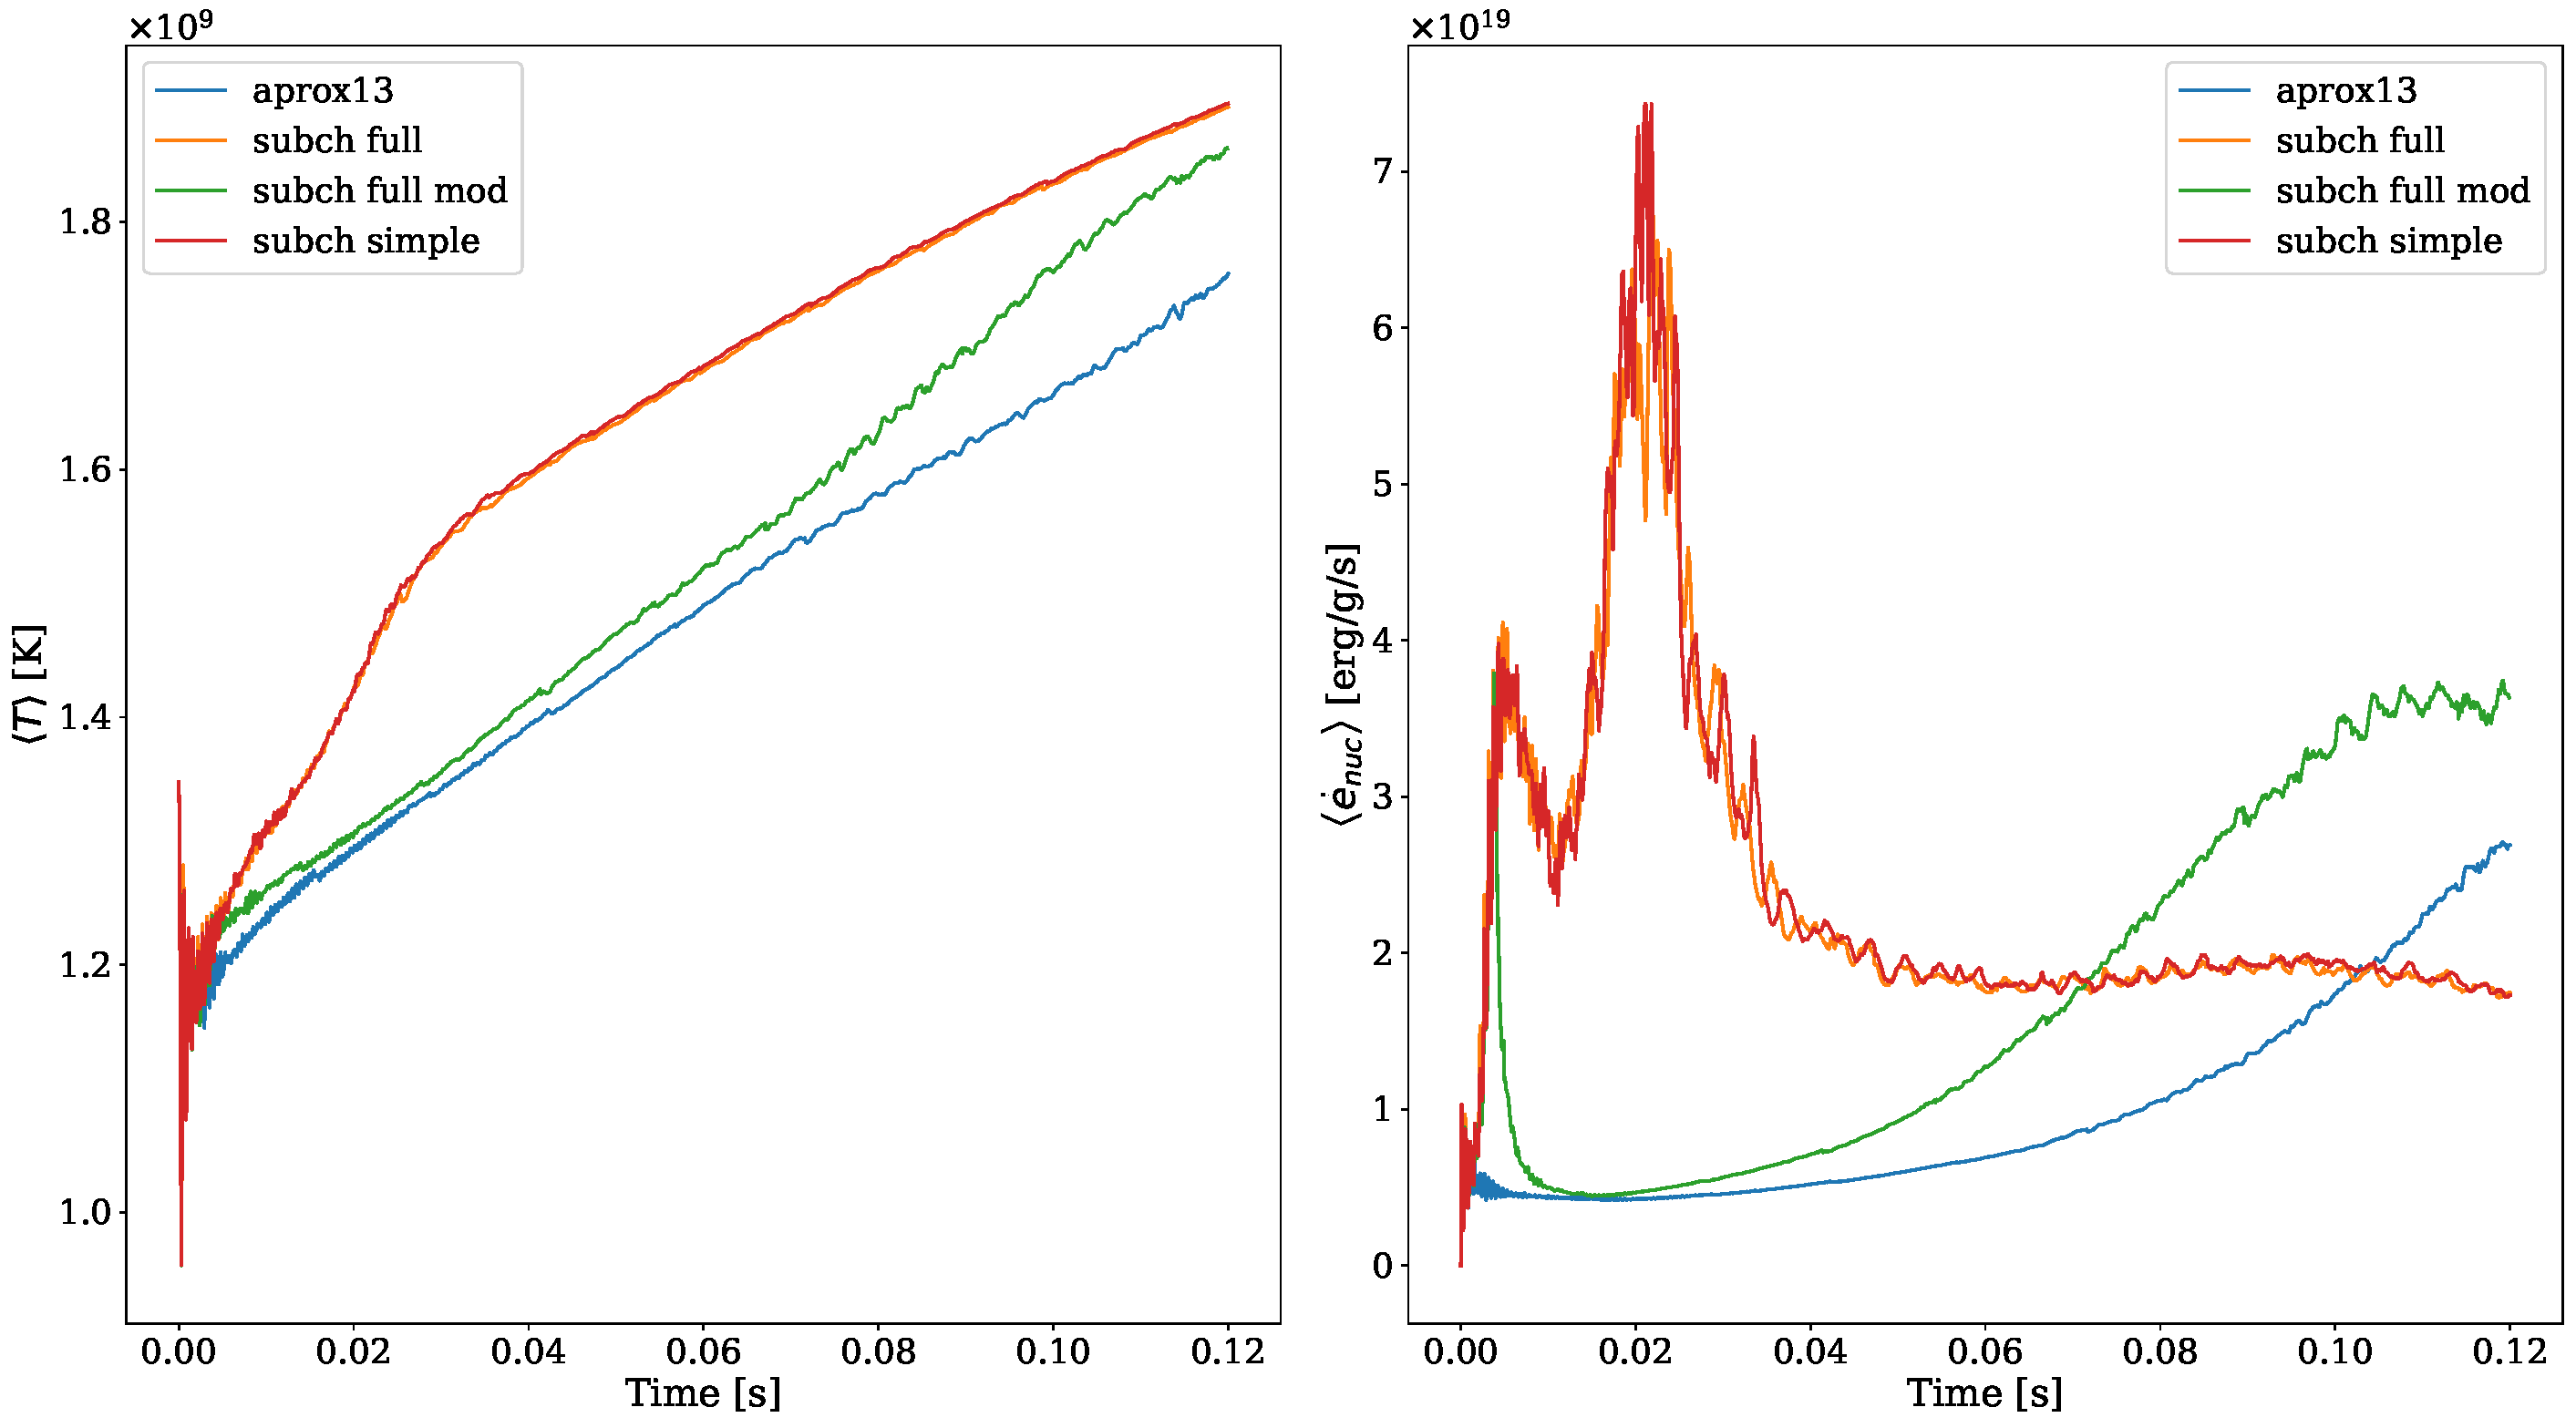
\includegraphics[width=1\linewidth]{network_time_profile.pdf}
        \caption{{\it Left}: The weighted temperature time profile. {\it Right}: The weighted nuclear energy generation rate time profile.}
    \end{figure}
\end{frame}


\begin{frame}
\frametitle{Results: Species Evolution Profiles}
    \begin{figure}
        \centering
        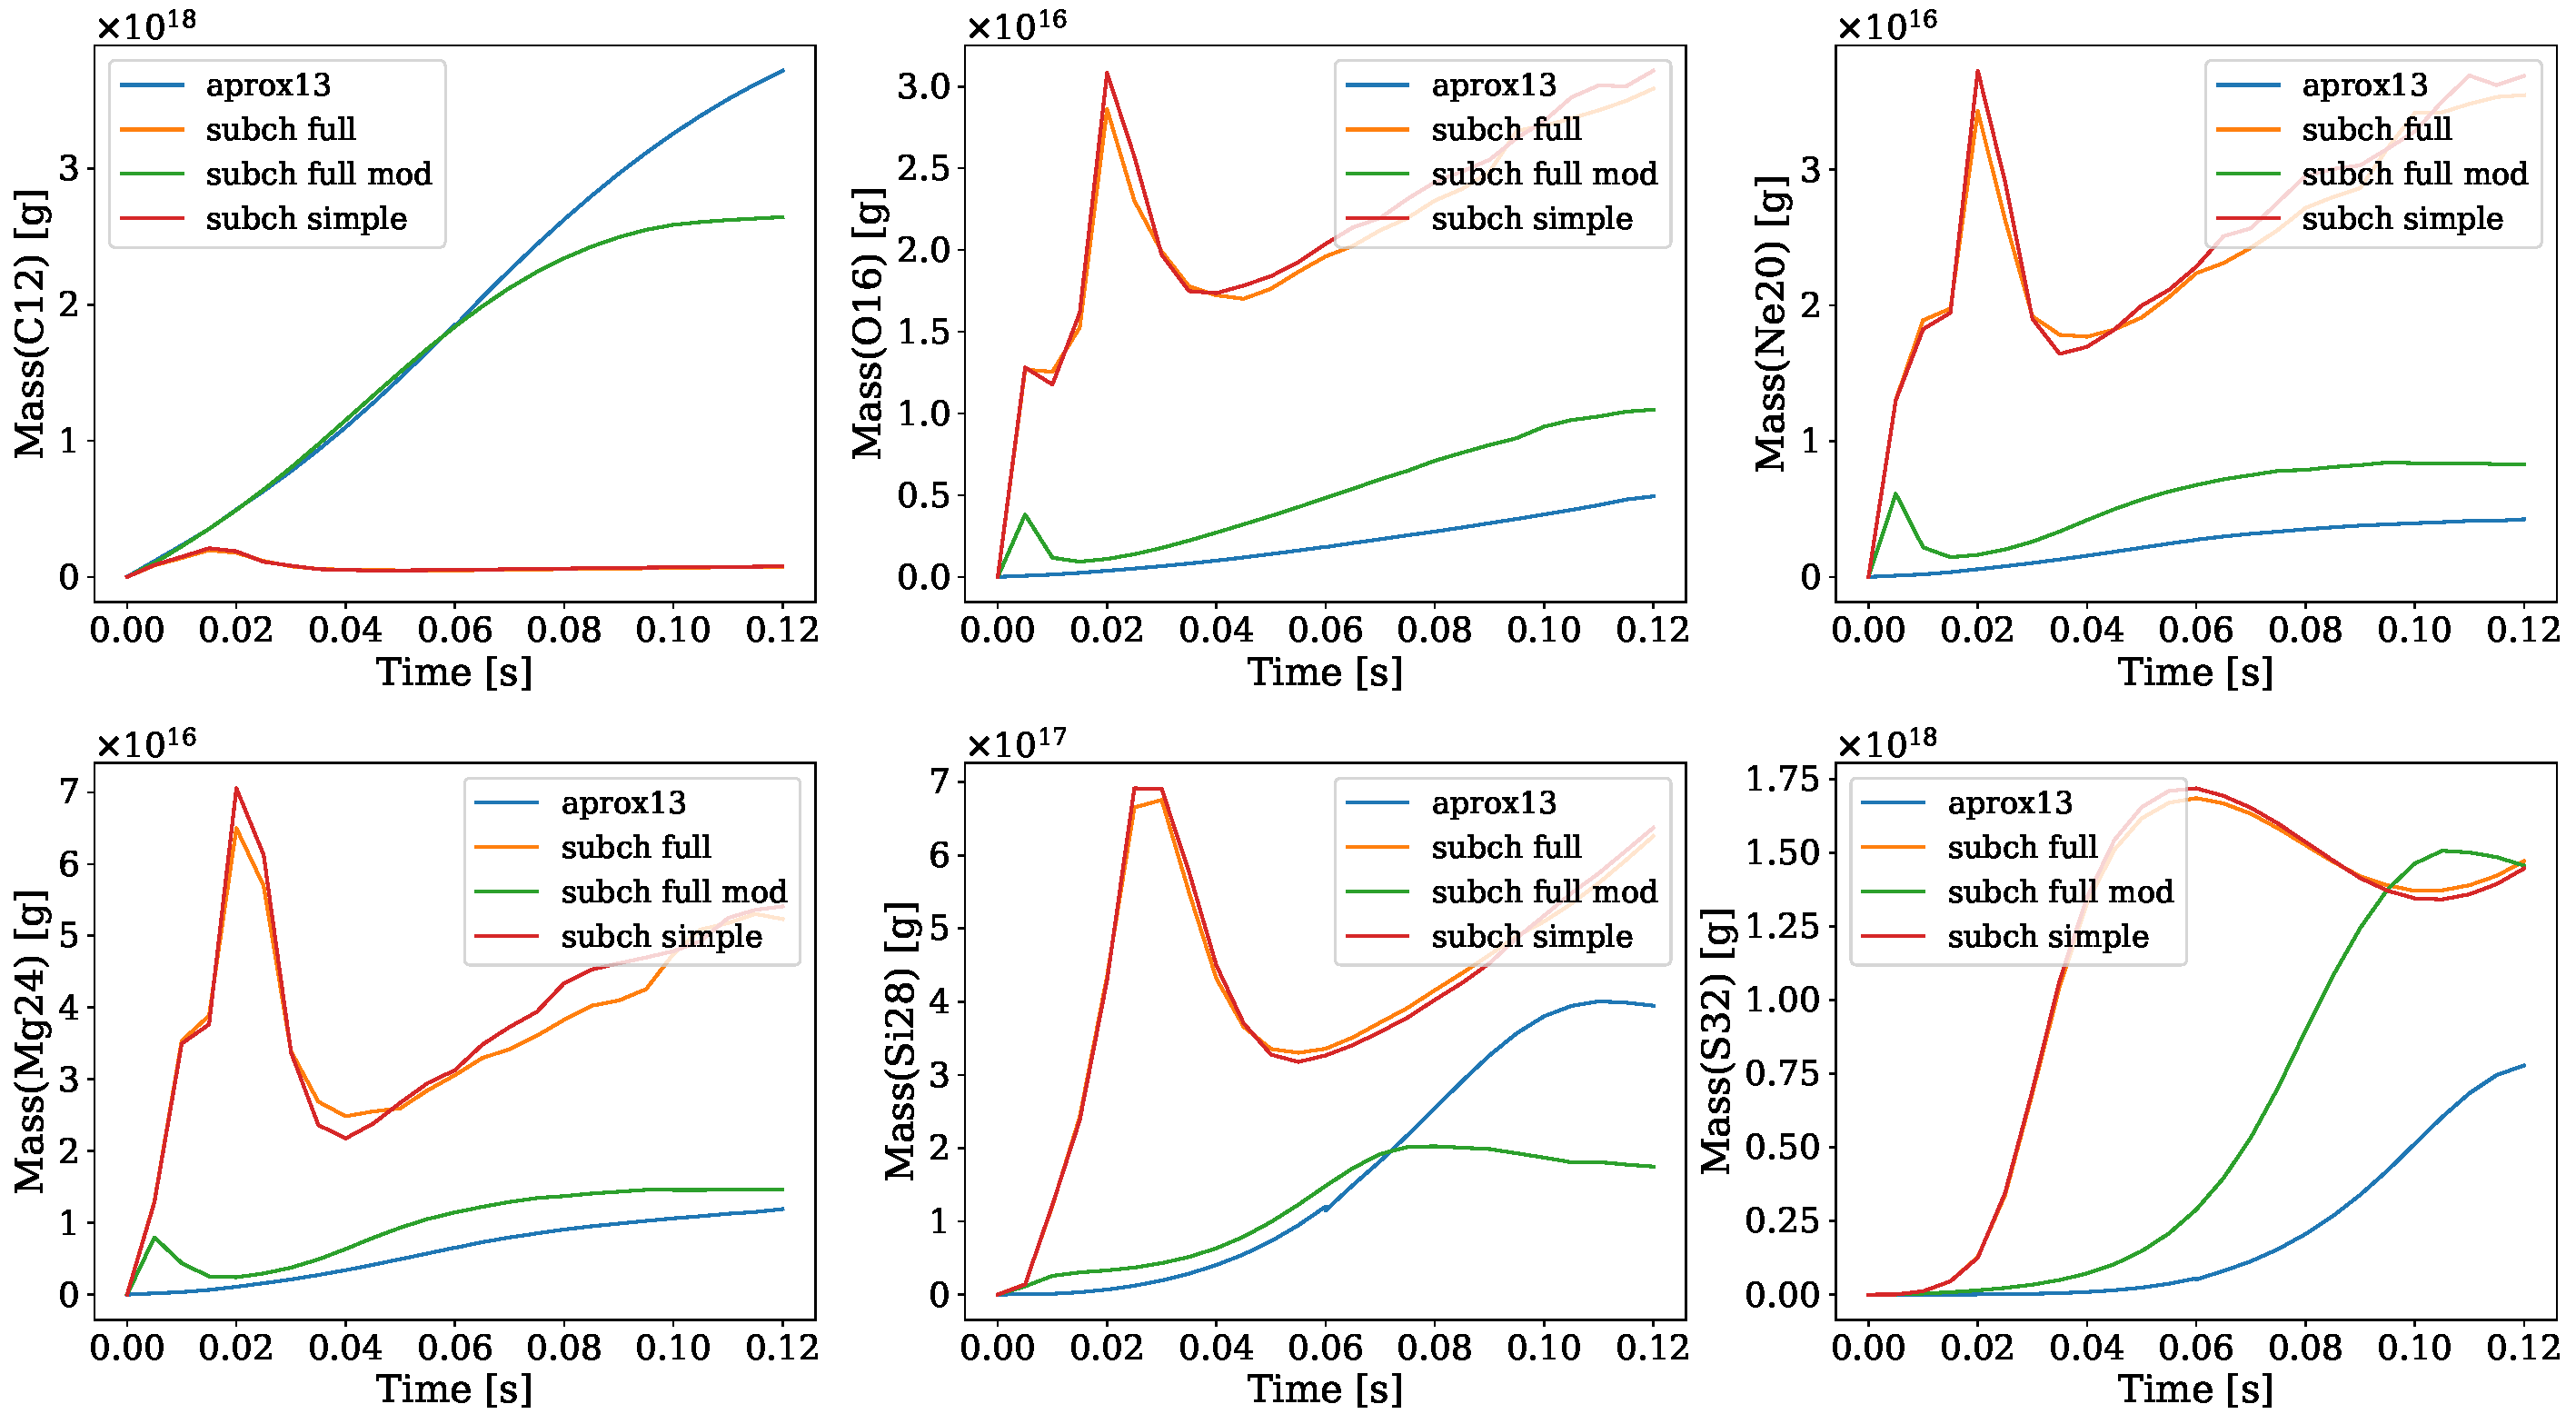
\includegraphics[width=1\linewidth]{network_species_summary.pdf}
        \caption{The evolution of the total mass for ${}^{12}$C, ${}^{16}$O, ${}^{20}$Ne,  ${}^{24}$Mg, ${}^{28}$Si, and ${}^{32}$S.}
    \end{figure}
\end{frame}


% \begin{frame}[allowframebreaks]
% \frametitle{Network: Mass fraction Comparison}
%     \begin{figure}
%         \centering
%         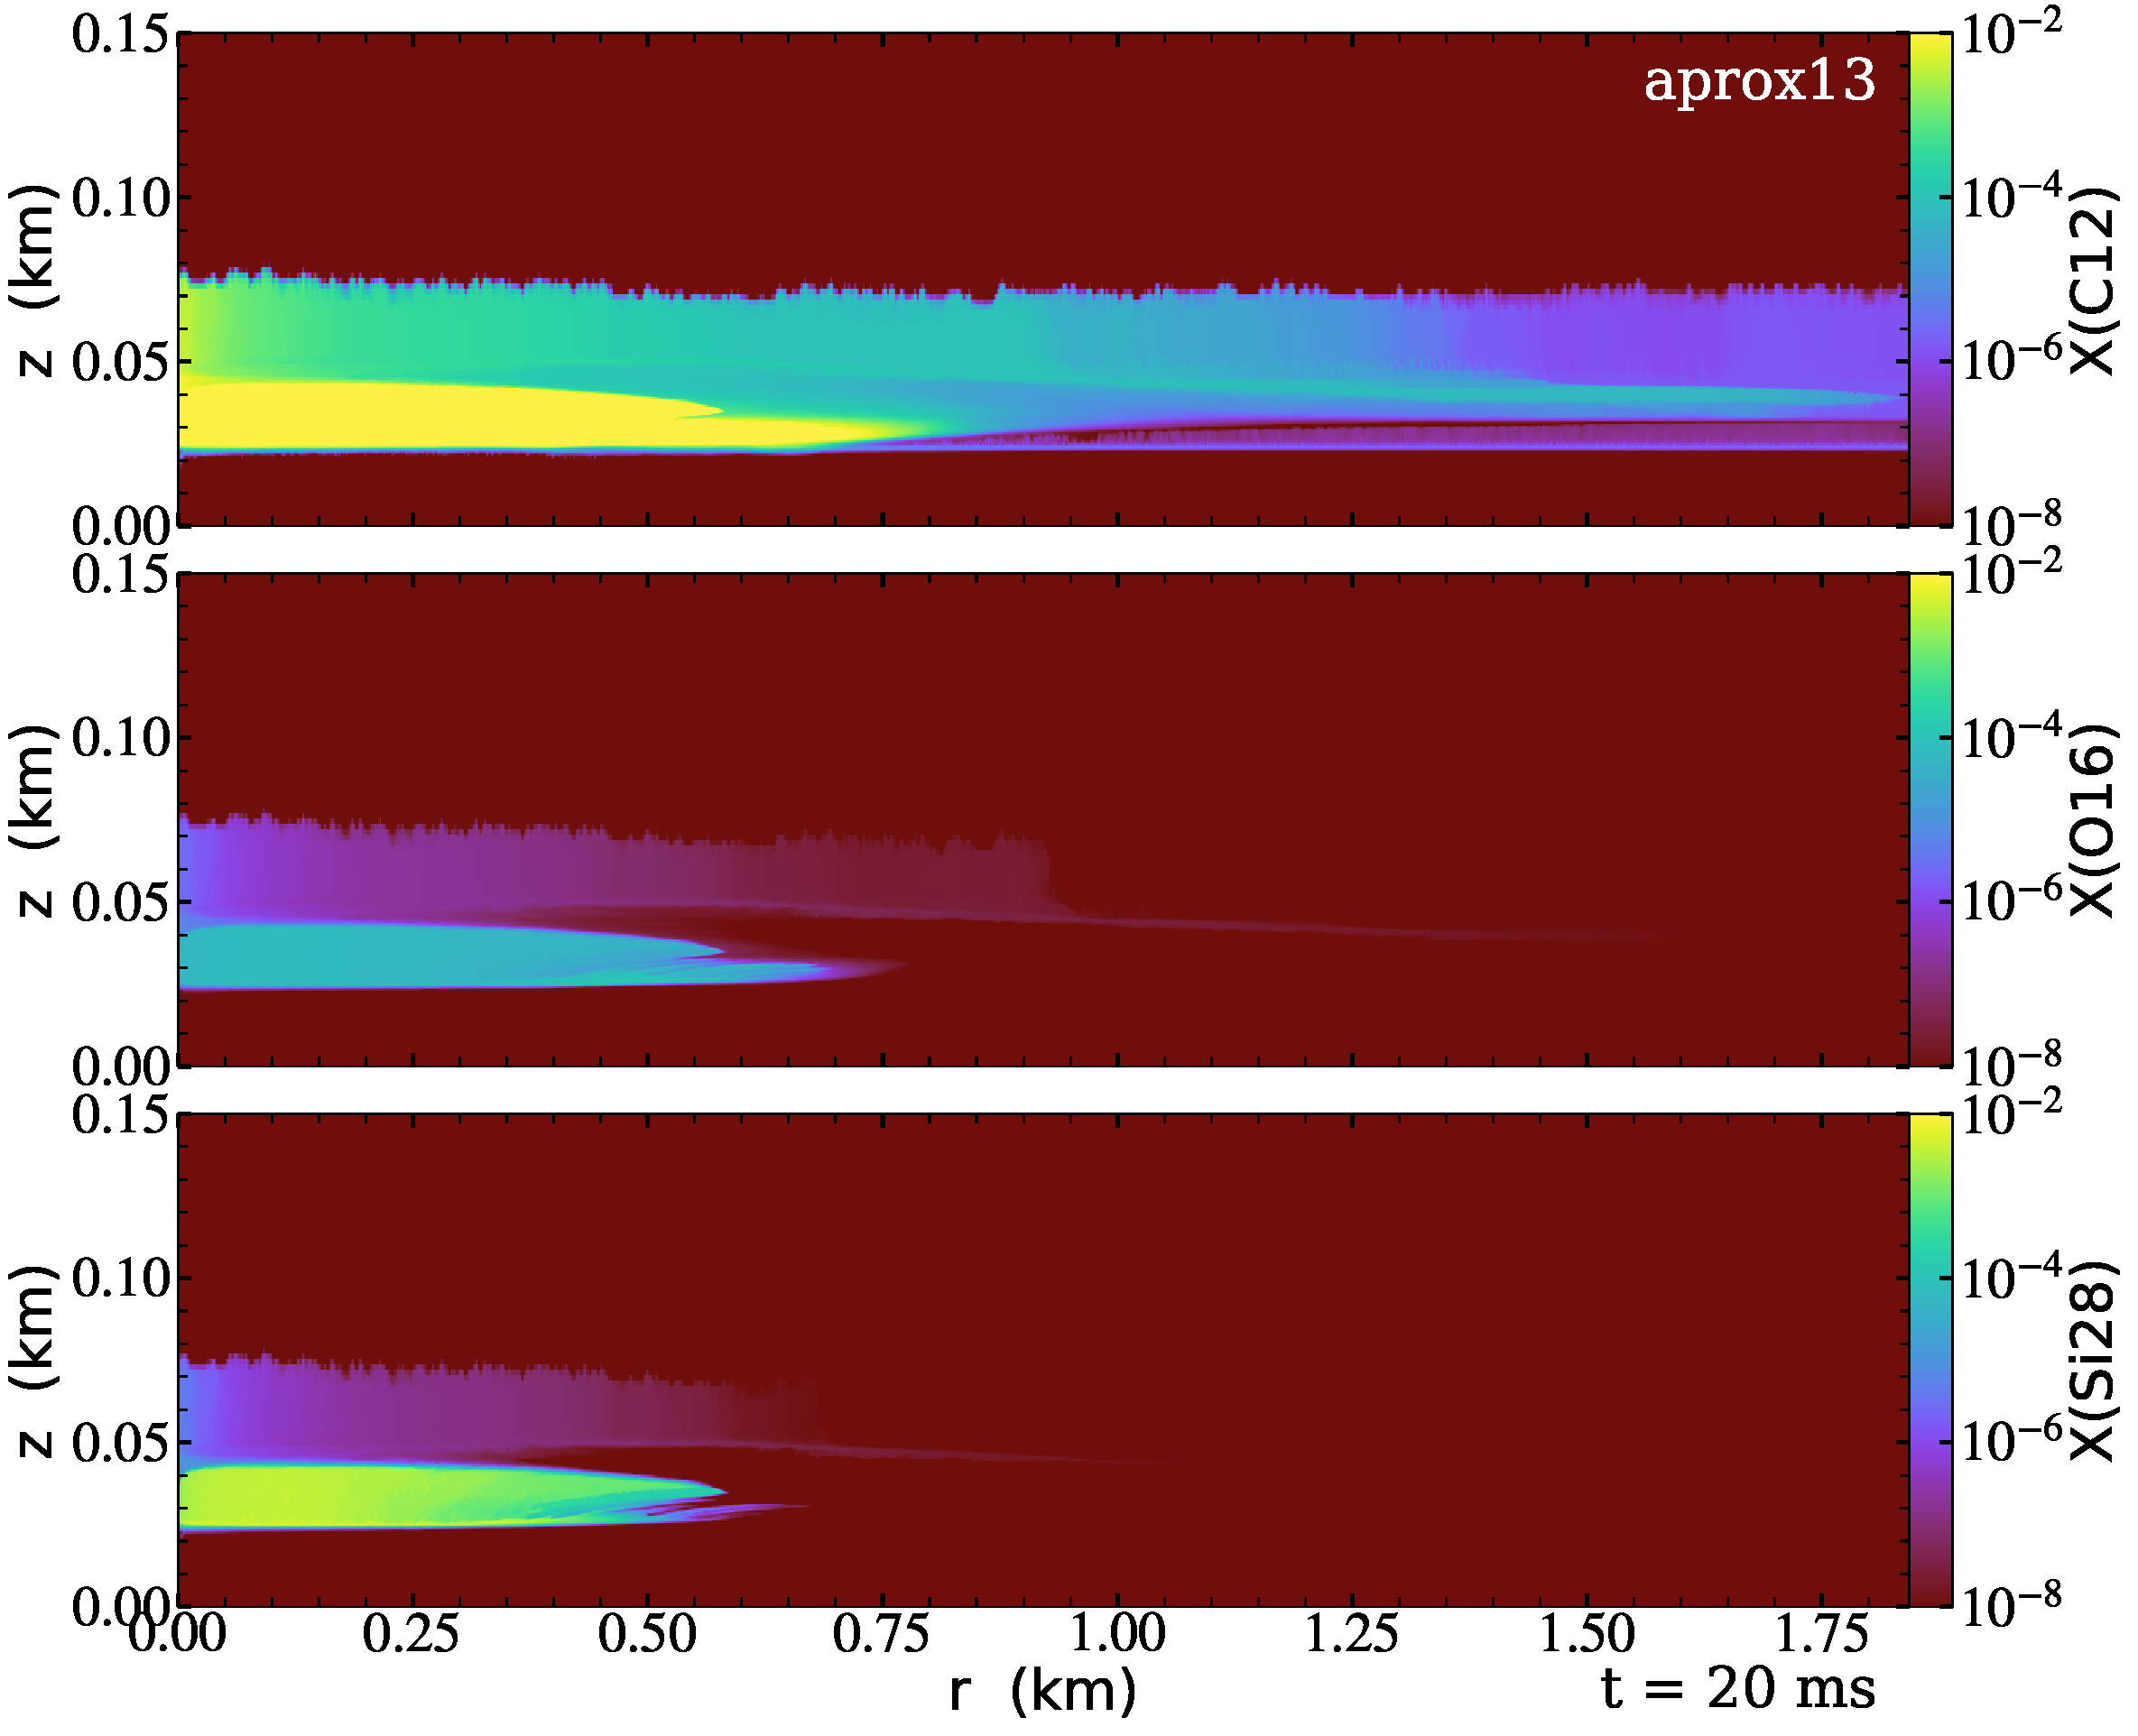
\includegraphics[width=0.8\linewidth]{network_aprox13_nuc_frac.pdf}
%         \caption{This figure shows the mass fractions of ${}^{12}$C, ${}^{16}$O, ${}^{20}$Ne,  ${}^{24}$Mg, ${}^{28}$Si, and ${}^{32}$S for {\tt aprox13} at 20 ms.}
%     \end{figure}
    
%     \begin{figure}
%         \centering
%         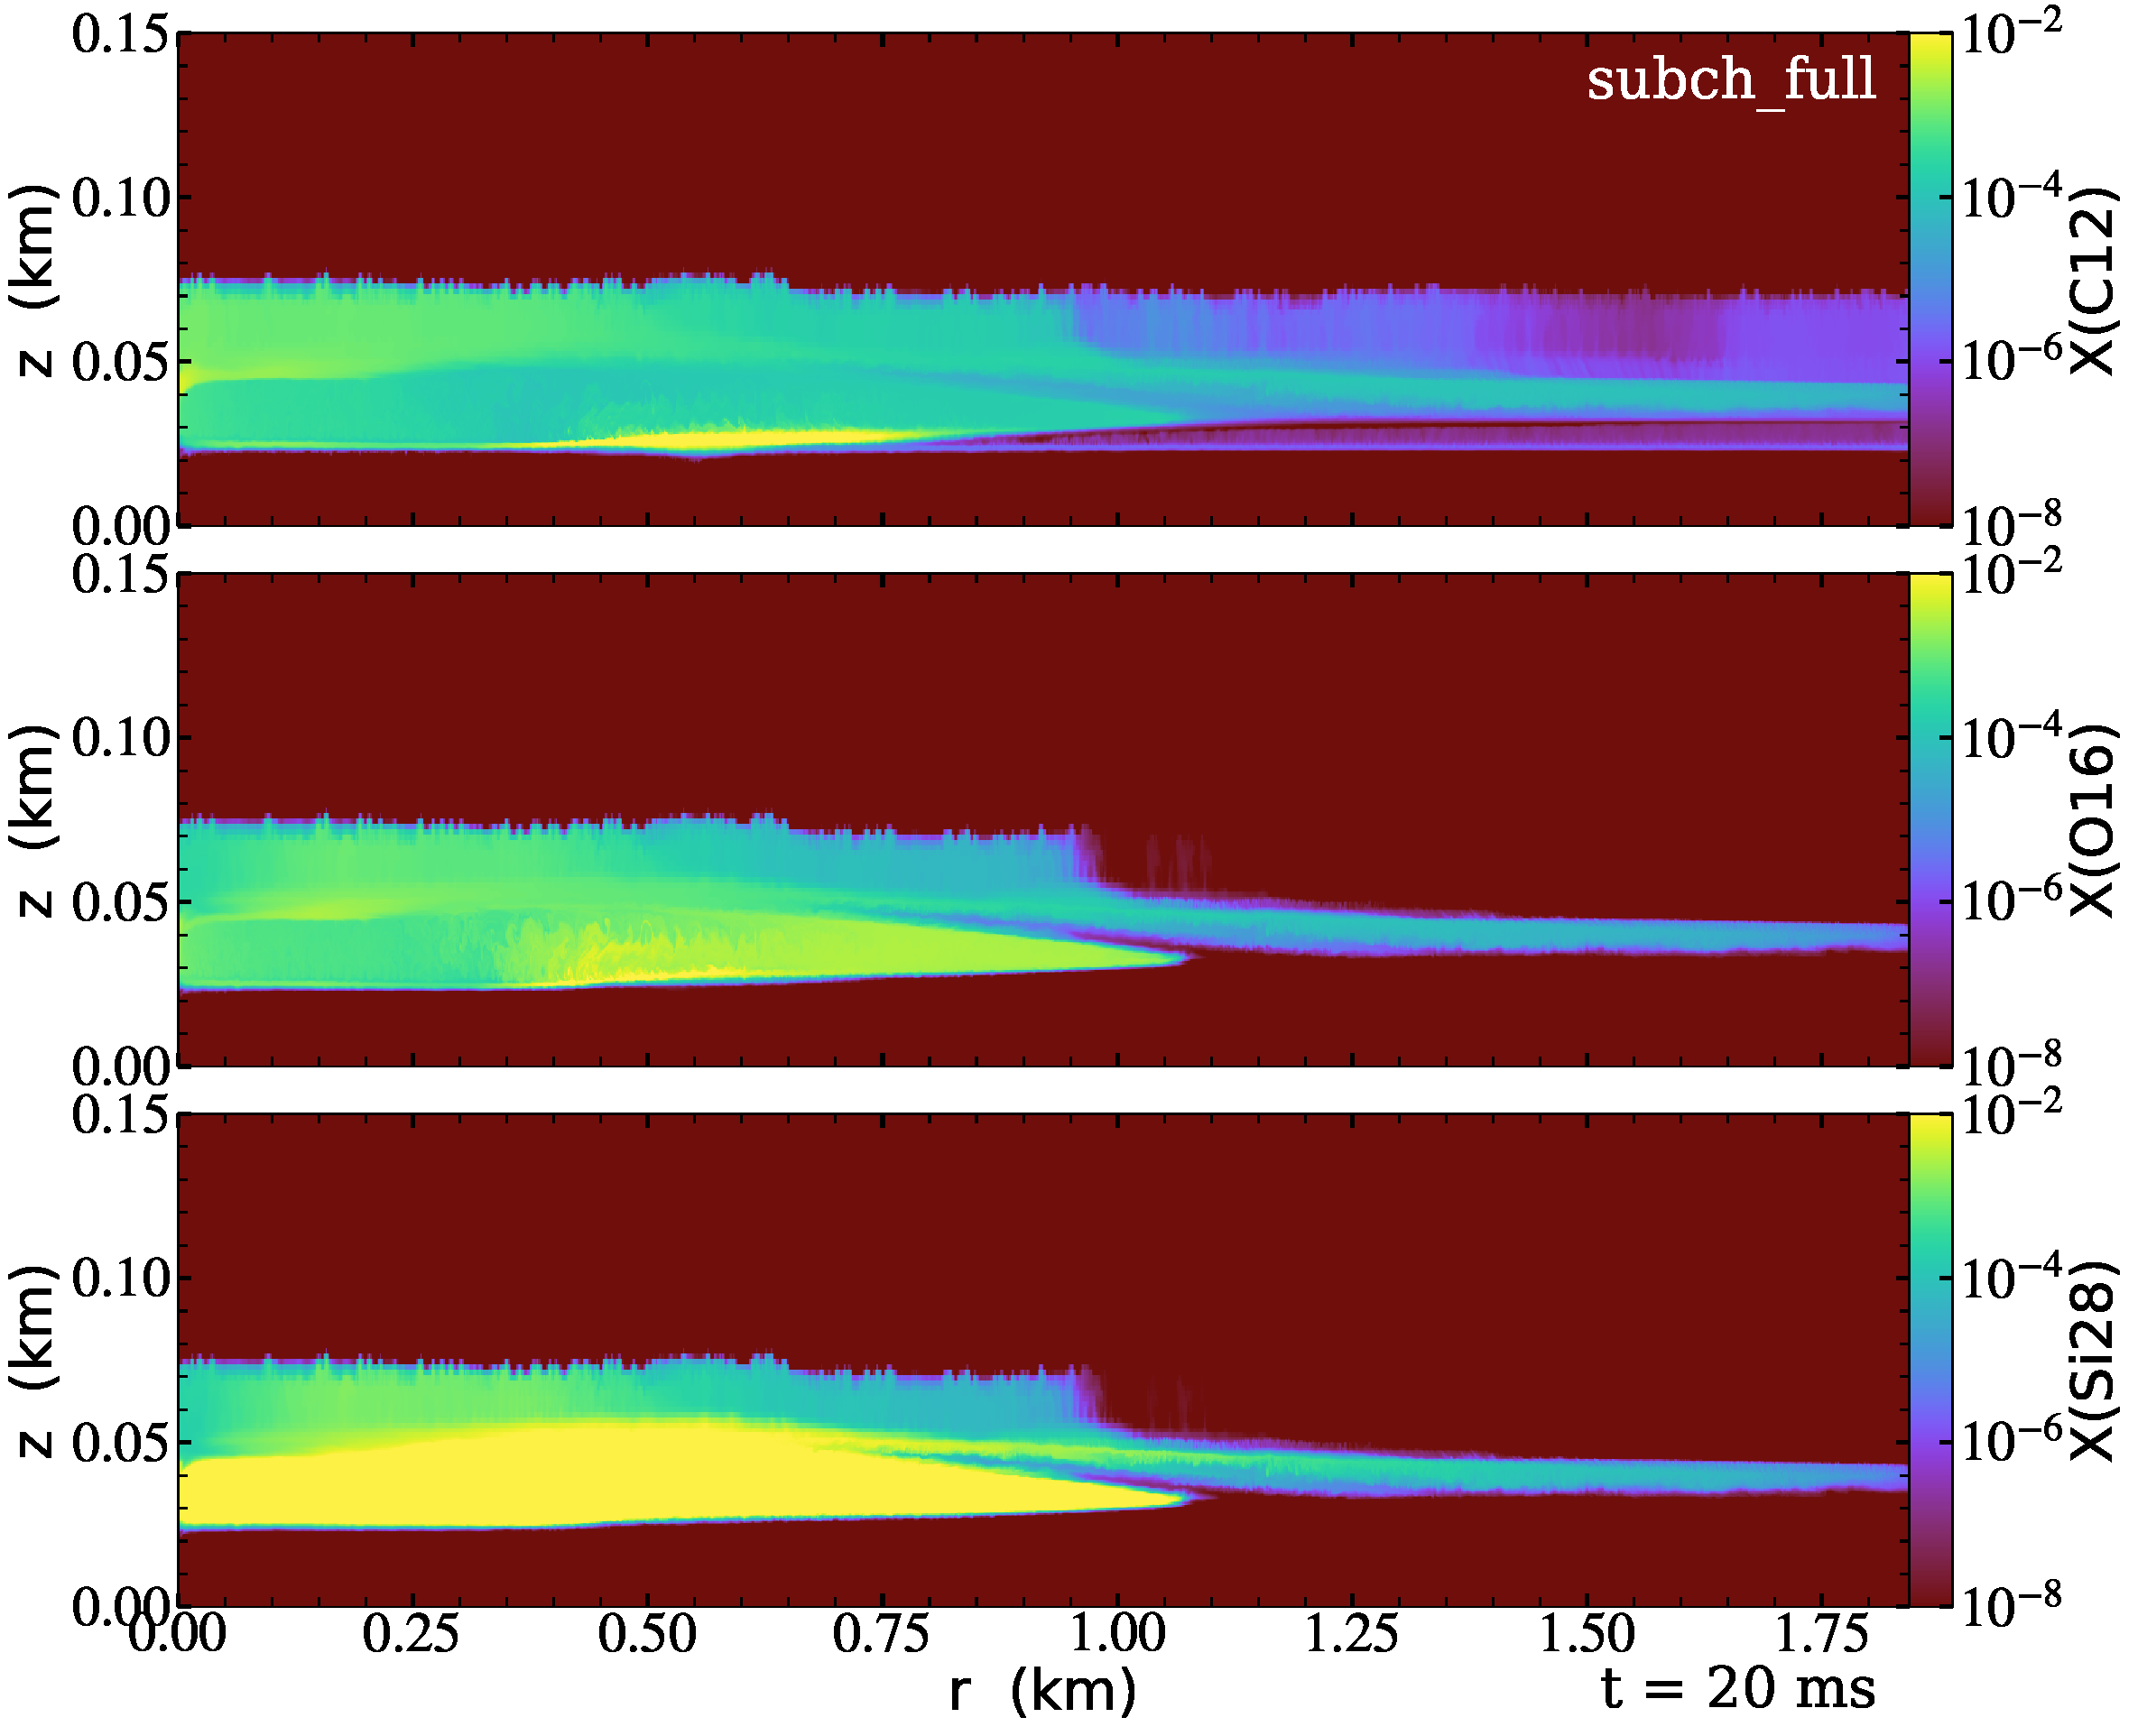
\includegraphics[width=0.8\linewidth]{network_subch_nuc_frac.pdf}
%         \caption{This figure shows the mass fractions of ${}^{12}$C, ${}^{16}$O, ${}^{20}$Ne,  ${}^{24}$Mg, ${}^{28}$Si, and ${}^{32}$S for {\tt subch full} at 20 ms.}
%     \end{figure}
    
%     \begin{figure}
%         \centering
%         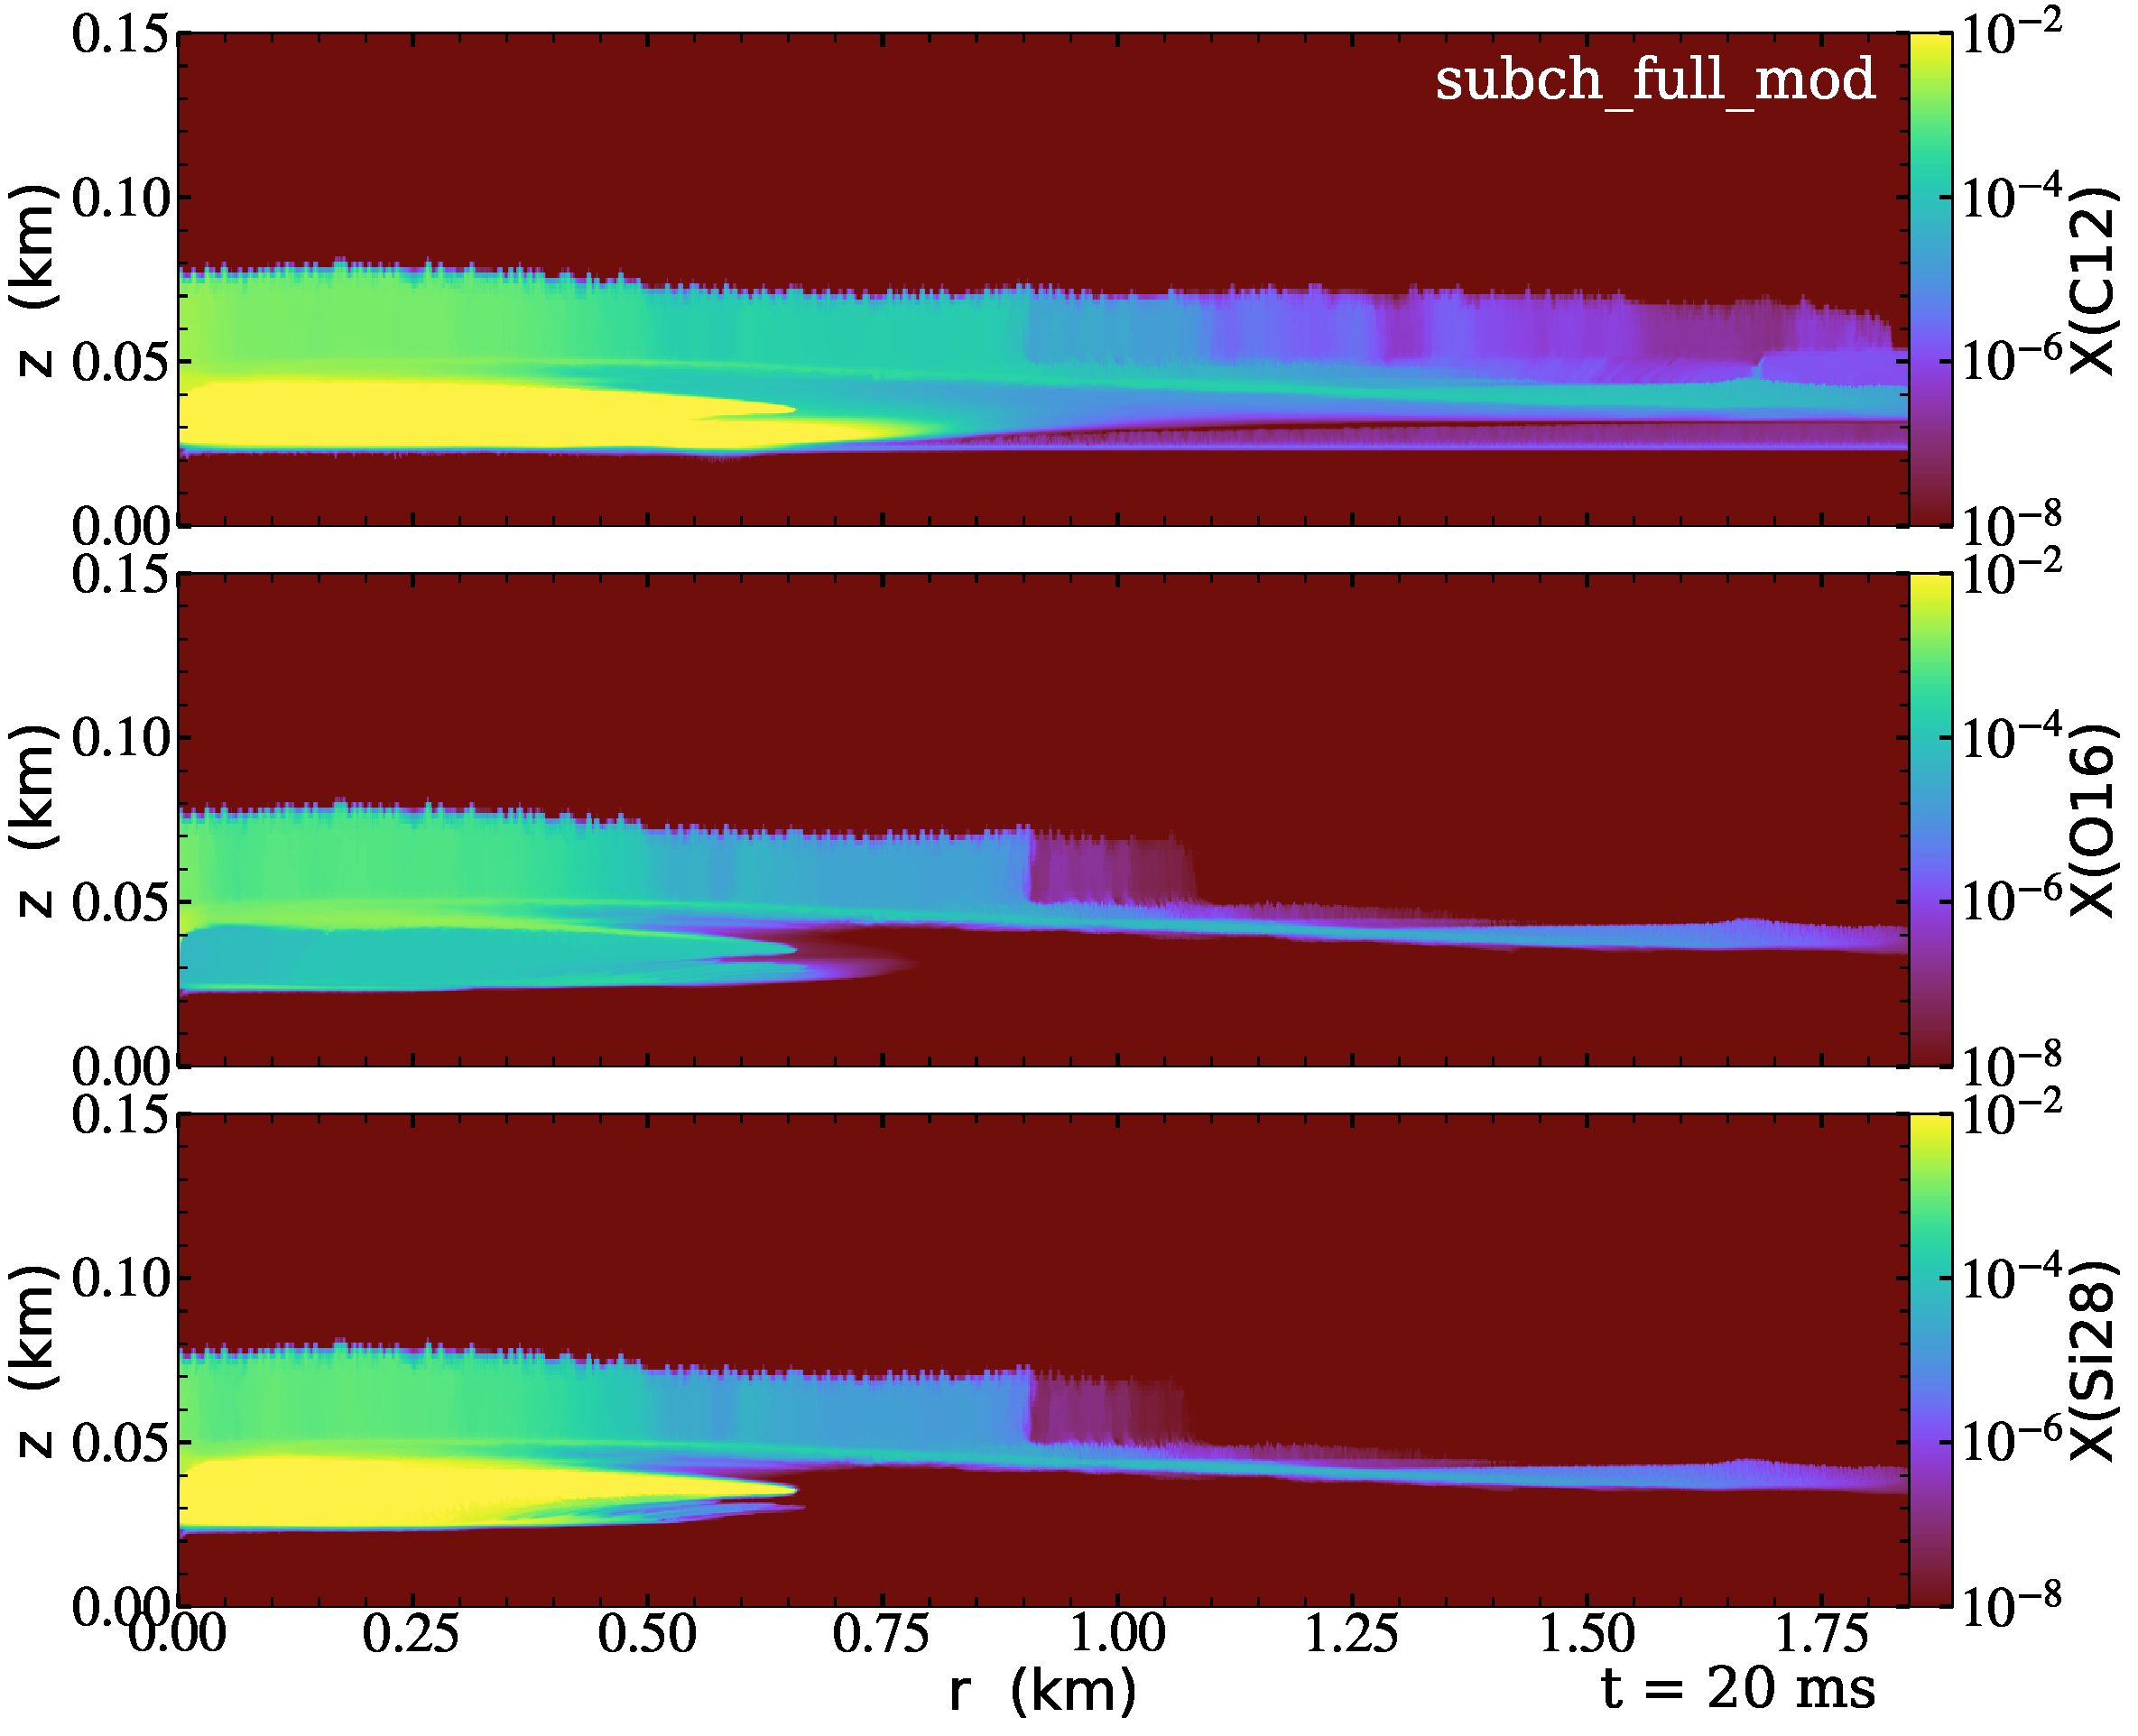
\includegraphics[width=0.8\linewidth]{network_subch_mod_nuc_frac.pdf}
%         \caption{This figure shows the mass fractions of ${}^{12}$C, ${}^{16}$O, ${}^{20}$Ne, ${}^{24}$Mg, ${}^{28}$Si, and ${}^{32}$S for {\tt subch full mod} at 20 ms.}
%     \end{figure}
    
% \end{frame}


% \begin{frame}
% \frametitle{\small Network: Weighted $T$ and $\dot{e}_{nuc}$ Time Profiles (Revisit)}
%     \begin{figure}
%         \centering
%         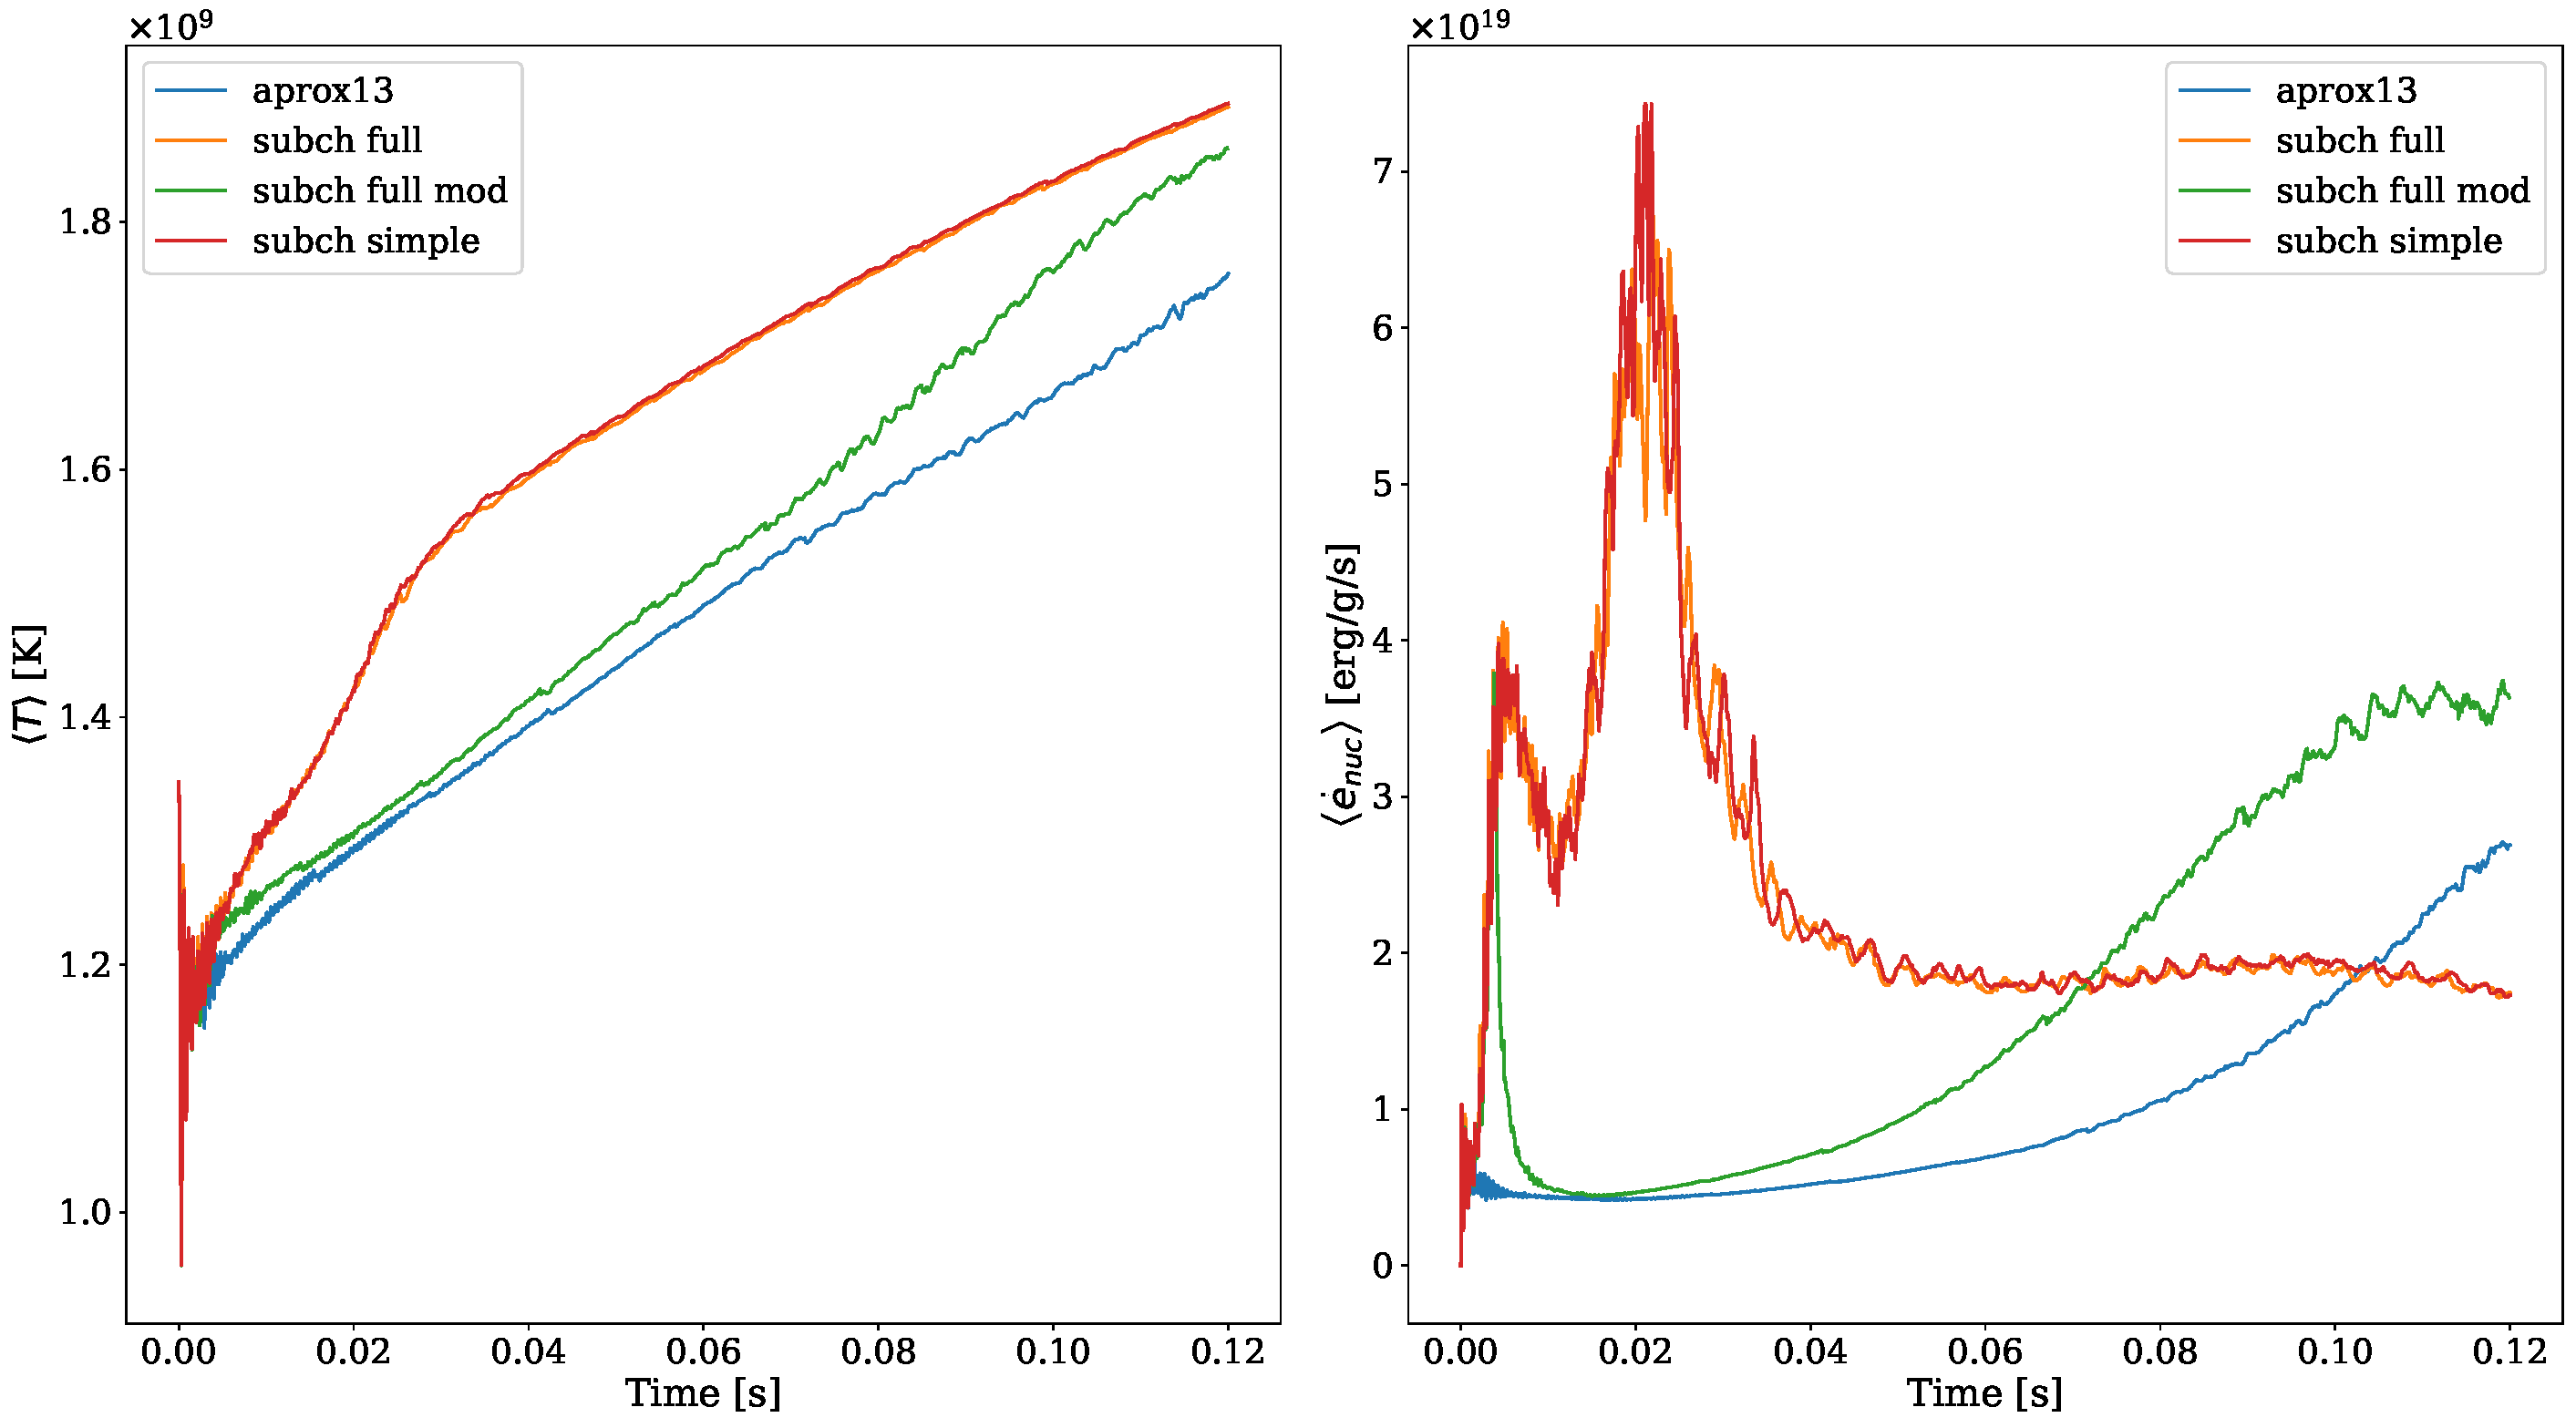
\includegraphics[width=1\linewidth]{network_time_profile.pdf}
%         \caption{{\it Left}: The weighted temperature time profile. {\it Right}: The weighted specific energy generation rate time profile.}
%     \end{figure}
% \end{frame}


\begin{frame}{Results: Front Position vs. Time}
%\begin{columns}
    %\column{1\linewidth}
    \begin{figure}
        \centering
        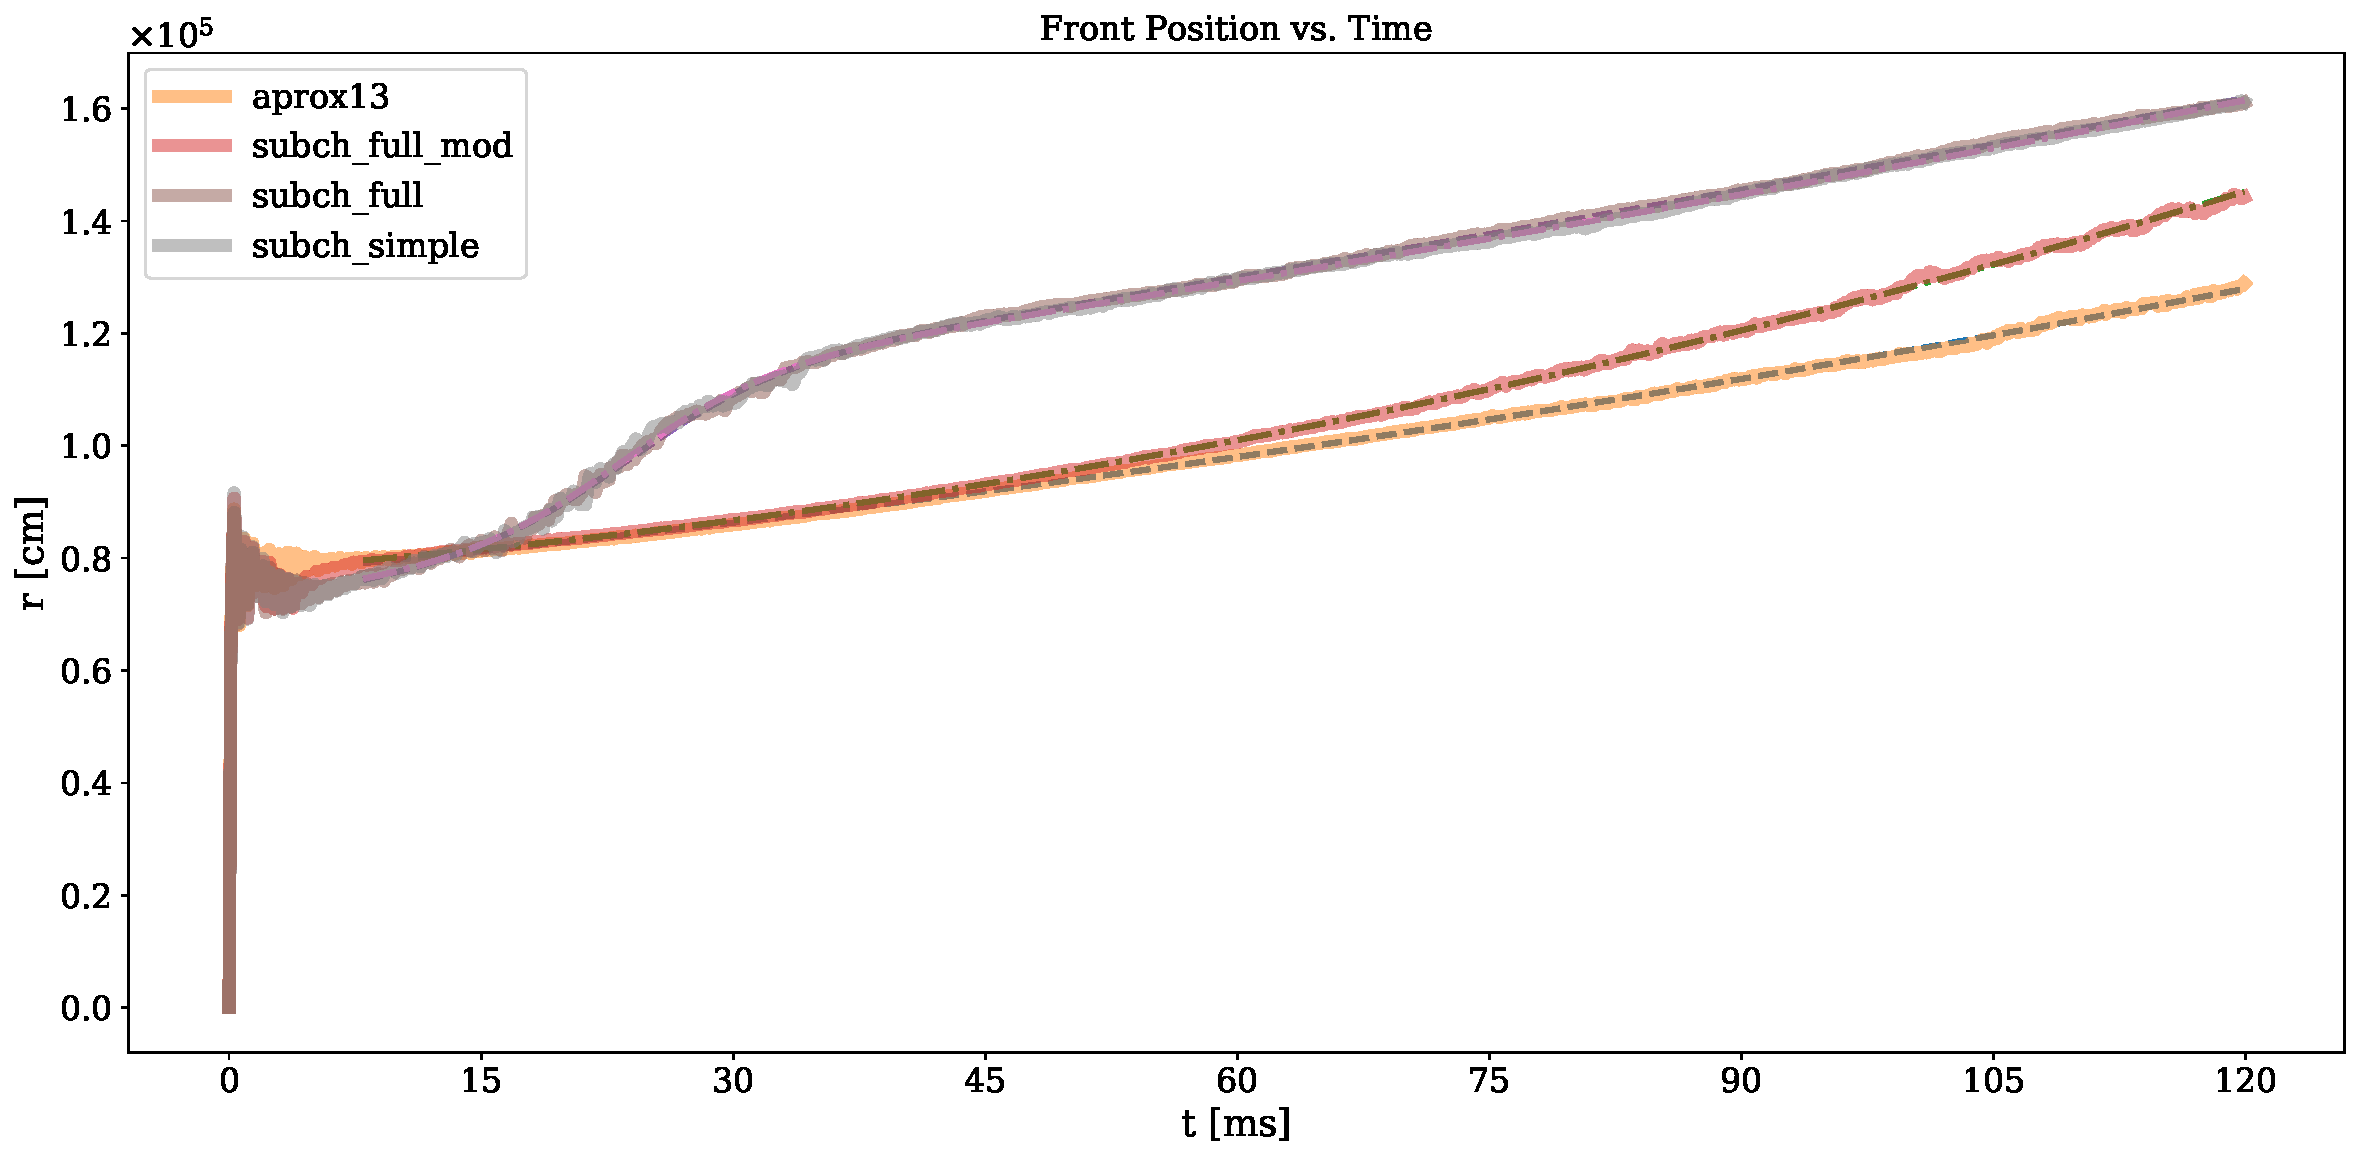
\includegraphics[width=1\linewidth]{network_front.pdf}
        \caption{The flame front position as a function time for {\tt aprox13}, {\tt subch full}, {\tt subch full mod}, and {\tt subch simple}. {\it Solid} Lines: Data. {\it Dashed} lines: fit.}
    \end{figure}
    
    % \column{0.2\linewidth}
    % \footnotesize The flame front position as a function time for {\tt aprox13}, {\tt subch full}, {\tt subch full mod}, and {\tt subch simple}. {\it Solid} Lines: Data, {\it Dashed} lines: fit.
%\end{columns}
    
\end{frame}


\begin{frame}[allowframebreaks]
\frametitle{Results: Flame Speed Comparison}

    % \begin{block}{Fitting Functions}
    %     \begin{subequations}
    %     \begin{equation}
    %          r(t) = \frac{1}{2}a_0 t^2 + v_0 t + r_0
    %     \end{equation}
        
    %     \begin{equation}
    %         r(t) = A\tanh{\left(\frac{t}{B} + C\right)} + \frac{1}{2}a_0 t^2 + v_0 t + r_0
    %     \end{equation}
    %     \end{subequations}
    % \end{block}
    
    % \begin{table}
    %     \resizebox{1\linewidth}{!}{
    %     \begin{tabular}{ccccccc}
    %     \toprule
    %     Name &
    %     $a_0$ [$\mbox{km} \ \mbox{s}^{-2}$] &
    %     $v_0$ [$\mbox{km} \ \mbox{s}^{-1}$] &
    %     $r_0$ [km] &
    %     A [$\mbox{km}$]&
    %     B [s]&
    %     C \\ 
    %     \midrule
    %     {\tt aprox13} & $24.22 \pm 0.23$ & $2.812 \pm 0.015$ & $0.7680\pm 0.0004 $ & N/A & N/A & N/A\\
        
    %     {\tt subch full} & $9.22 \pm 0.82$ & $4.489 \pm 0.067$ & $0.8646 \pm 0.0014$ & $0.150 \pm 0.001$ & $0.0093 \pm 0.0001$ & $-2.551 \pm 0.035$ \\
        
    %     {\tt subch full mod} & $58.53 \pm 0.24$ & $2.122 \pm 0.016$ & $0.7773 \pm 0.0004$ & N/A & N/A & N/A \\
        
    %     {\tt subch simple} & $15.60 \pm 0.93$ & $3.961 \pm 0.076$ & $0.8745 \pm 0.0016$ & $0.153 \pm 0.002$ & $0.0091 \pm 0.0001$ & $-2.575 \pm 0.040$\\
         
    %     %{\tt aprox13 chu} & $22.96 \pm 0.20$ & $2.578 \pm 0.0133$ & $0.7728 \pm 0.0004$ & N/A & N/A & N/A\\
         
    %     %{\tt aprox13 sdc} & $28.09 \pm 0.20$ & $2.392 \pm 0.013$ & $0.7836\pm 0.0004 $ & N/A & N/A & N/A\\
        
    %     %{\tt subch full sdc} & $2.34 \pm 0.74$ & $4.947 \pm 0.061$ & $0.8601 \pm 0.0013$ & $0.146 \pm 0.001$ & $0.0098 \pm 0.0001$ & $-2.424 \pm 0.030$ \\
    %     \bottomrule
    %     \end{tabular}}
    %     \caption{This table shows the fitted parameters of the fitting functions. The fitting function is applied for $t > 8$ ms.}
    % \end{table}

    \begin{table}
        \resizebox{1\linewidth}{!}{
        \begin{tabular}{cccc}
        \toprule 
        \scriptsize
        Name &
        $v_{23}$ [$\mbox{km} \ \mbox{s}^{-1}$] &
        $v_{100}$ [$\mbox{km} \ \mbox{s}^{-1}$] &
        $t_{10}$ [s]\\
        \midrule
        {\tt aprox13} & $3.369 \pm 0.016$ & $5.234 \pm 0.027$ & 0.7647\\
        {\tt subch full} & $20.732 \pm 0.284$ & $5.411 \pm 0.105$ & 0.9917 \\
        {\tt subch full mod} & $3.468 \pm 0.017$ & $7.975 \pm 0.029$ & 0.4873\\
        {\tt subch simple} & $21.095 \pm 0.332$ & $5.521 \pm 0.120$ & 0.8483\\
        \bottomrule
        \end{tabular}}
        \caption{This table shows the instantaneous flame propagation speed at $t = 23$ ms and $t = 100$ ms calculated using the fitting function. $t = 23$ ms represents the acceleration for {\tt subch full} and {\tt subch simple}. $t = 100$ ms represents the steady phase at the late-stage. $t_{10}$ shows the expected time for the flame to reach $r=10$ km using the fitting function.}
    \end{table}

\end{frame}


% \section{Plasma Screening Routines}
% \subsection{Overview of Screening Routines}


% \begin{frame}{Plasma Screening}
%     \begin{center}
%         \Huge {\it Effect of different plasma screening routines}
%     \end{center}
% \end{frame}

% \begin{frame}{Plasma Screening Introduction}
%     \begin{block}{What is plasma screening?}
%         \begin{itemize}
%             \item Plasma screening enhances the nuclear reaction rate by reducing the Coulomb barrier that reacting nuclei must overcome. 
%             \item The overall screening regime depends on the Coulomb coupling parameter, $\Gamma \propto \frac{((Z_1 +Z_2))^{1/3}}{Z_1Z_2} \Gamma_{e}$ with $\Gamma_e \propto \frac{n_e^{1/3}}{T}$ 
%         \end{itemize}
%     \end{block}
    
%     \begin{block}{Screening Regimes}
%     \begin{itemize}
%         \item Weak Screening: $\Gamma \ll 1$
%         \item Strong Screening: $\Gamma \gtrsim 1$
%     \end{itemize}
%     \end{block}
    
%     \begin{equation}\label{Eq:screening}
%         R_{scr} = F_{scr} R_{th}
%     \end{equation}
% \end{frame}

% \begin{frame}
% \frametitle{{\tt SCREEN5} vs. {\tt CHUGUNOV2007}}

%     \begin{block}{\tt SCREEN5}
%         \begin{itemize}
%             \item {\it Weak} Regime $(\Gamma < 0.3)$: Follows Graboske 1973\cite{Graboske_1973}. Assumes interacting nuclei are separated by zero distance.
%             \item {\it Strong} Regime $(\Gamma > 0.8)$: Follows Alastuey \& Jancovici (AJ) 1978 \cite{Alastuey_Jancovici:1978}. Assumes a quadratic dependence of the separation distance between interacting nuclei.
%             \item {\it Intermediate} Regime $(0.3 < \Gamma < 0.8)$: A weighted value between both weak and strong regime calculations.
%         \end{itemize}
%     \end{block}

%     \begin{block}{\tt CHUGUNOV2007}
%         \begin{itemize}
%             \item Follows Chugunov 2007 \cite{Chugunov_2007}.
%             %\item Assumes a higher order polynomial dependence of the separation distance between interacting nuclei.
%             \item Assumes WKB Coulomb barrier penetration through the radial mean-field potential.
%             \item A single expression for all screening regimes.
%         \end{itemize}
%     \end{block}
% \end{frame}

% \begin{frame}{Plasma Screening: Models}
%     % \begin{center}
%     %     \LARGE Plasma Screening
%     % \end{center}
    
%     \begin{table}
%         \resizebox{1\linewidth}{!}{
%         \begin{tabular}{cccc}
%         \toprule
%         Name &
%         Network &
%         Integration &
%         Screening\\ 
%         \midrule
        
%         {\tt aprox13} & {\tt aprox13} & strang-splitting & {\tt SCREEN5} \\
%         % {\tt subch full} & {\tt subch full} & strang-splitting & {\tt SCREEN5} \\
%         % {\tt subch full mod} & {\tt subch full mod} & strang-splitting & {\tt SCREEN5} \\
%         % {\tt subch simple} & {\tt subch simple} & strang-splitting & {\tt SCREEN5} \\
%         % {\tt aprox13 sdc} & {\tt aprox13} & simplified SDC & {\tt SCREEN5} \\
%         % {\tt subch full sdc} & {\tt subch full} & simplified SDC & {\tt SCREEN5} \\
%         {\tt aprox13 chu} & {\tt aprox13} & strang-splitting & {\tt CHUGUNOV2007} \\
%         \bottomrule
%         \end{tabular}}
%         \caption{This table shows the various settings used for each simulation.}
%     \end{table}
    
% \end{frame}

% \subsection{Simulation Results}

% \begin{frame}{Screening: $\Bar{A}$ and $T$ Comparison}
%     \begin{figure}
%         \centering
%         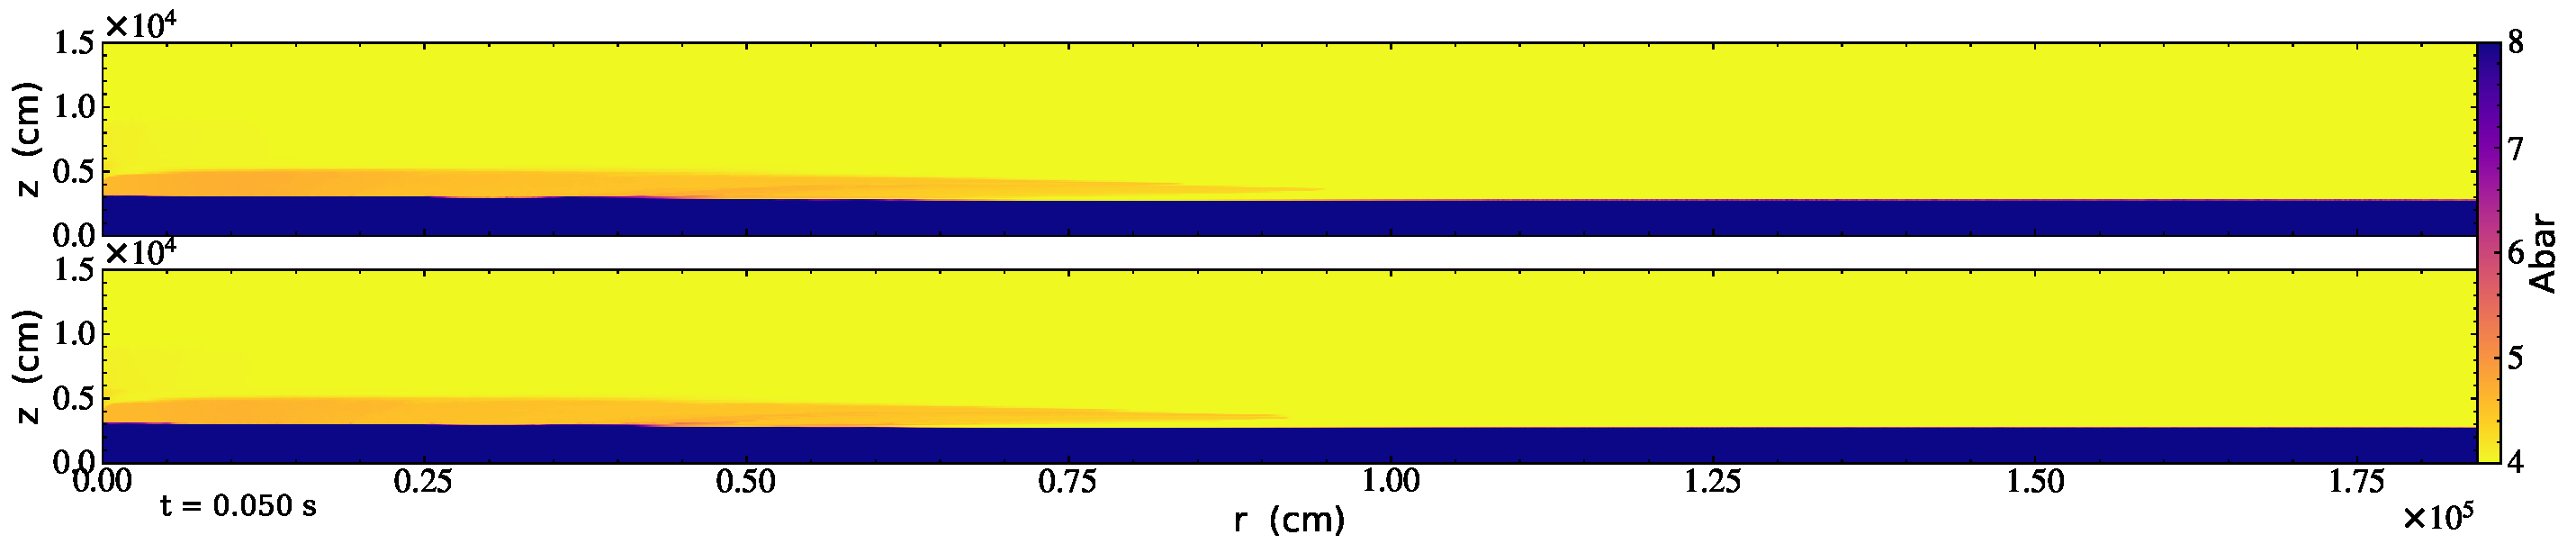
\includegraphics[width=1\linewidth]{screen_abar_50ms.pdf}
%         \caption{{\it Top}: $\Bar{A}$ for {\tt aprox13}. {\it Bot}: $\Bar{A}$ for {\tt aprox13 chu}}
%     \end{figure}
    
%     \begin{figure}
%         \centering
%         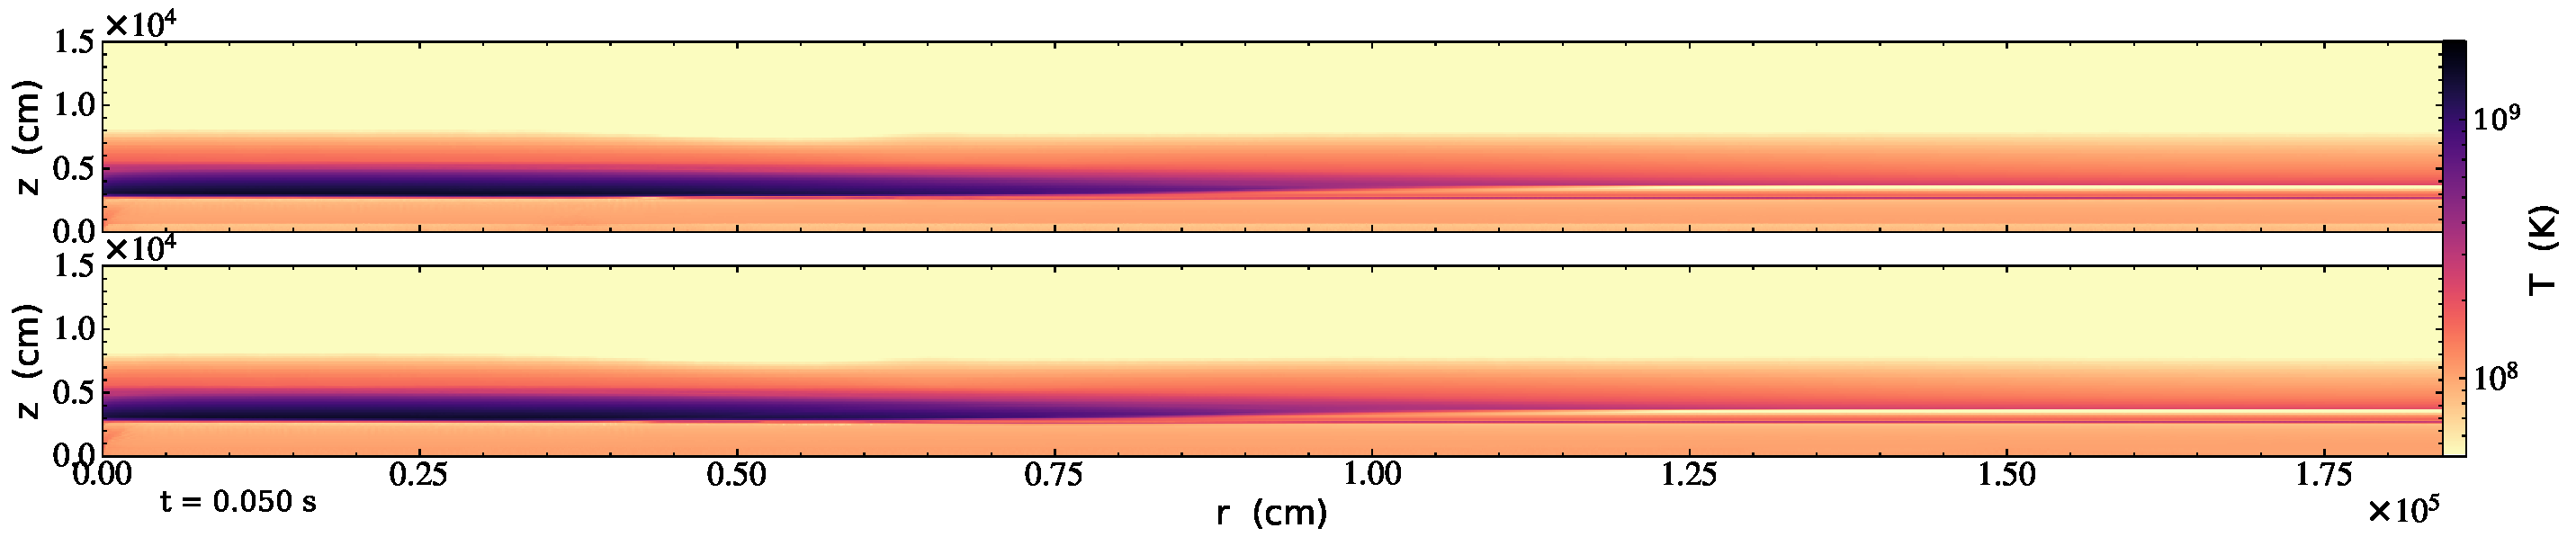
\includegraphics[width=1\linewidth]{screen_temp_50ms.pdf}
%         \caption{{\it Top}: $T$ for {\tt aprox13}. {\it Bot}: $T$ for {\tt aprox13 chu}}
%     \end{figure}
% \end{frame}


% \begin{frame}{Screening: $\Gamma$ Comparison}
% \begin{columns}
%     \column{0.75\linewidth}
    
%     \begin{figure}
%         \centering
%         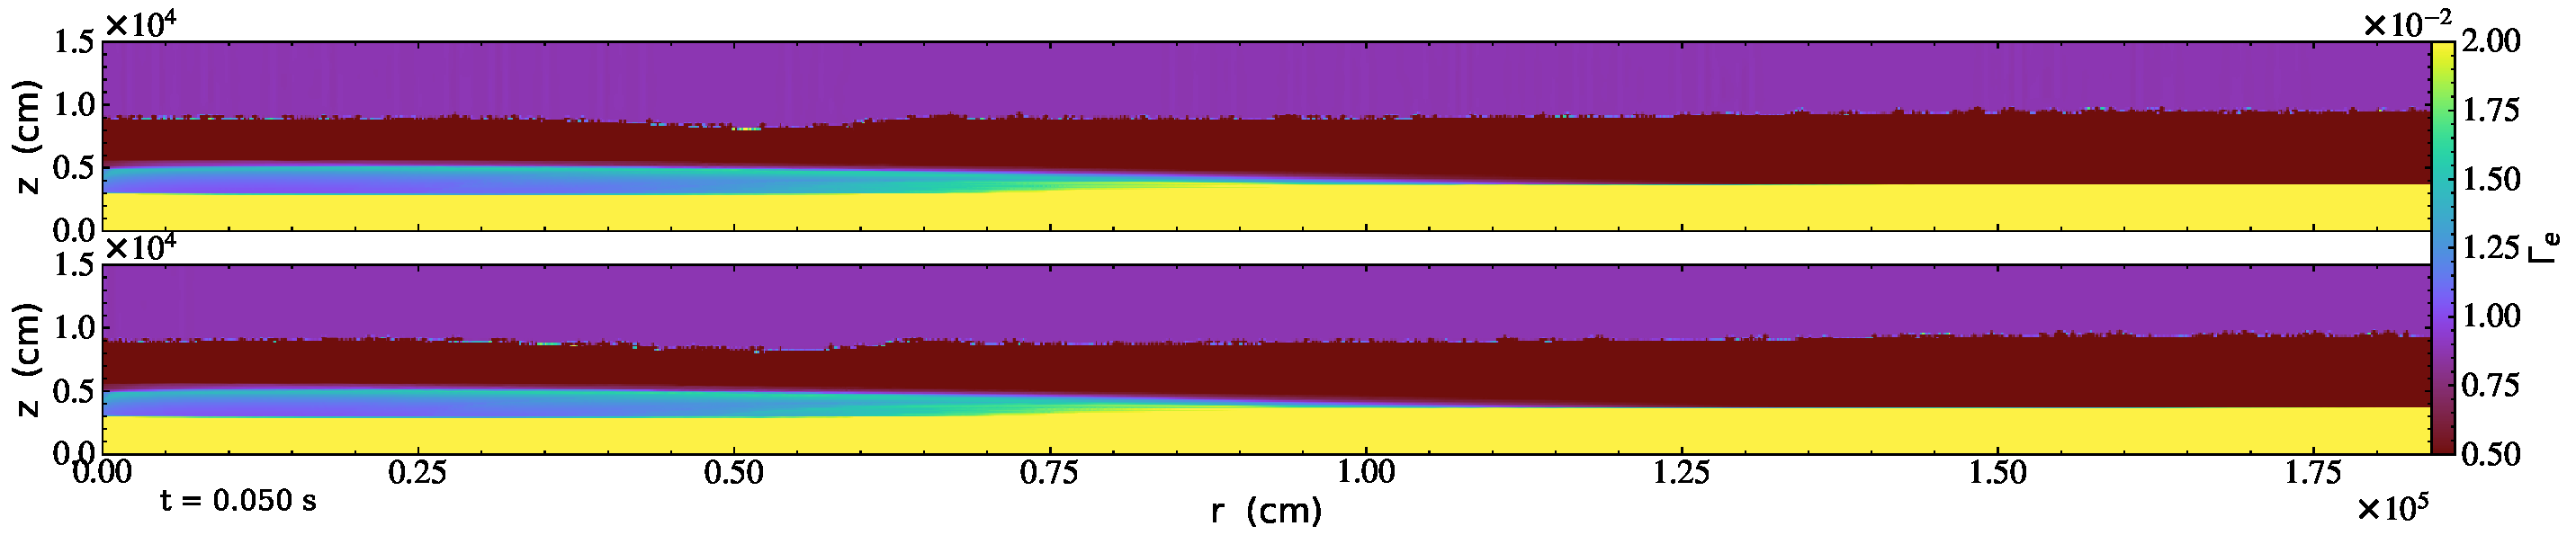
\includegraphics[width=1\linewidth]{screen_gamma_50ms.pdf}
%         \caption{\scriptsize {\it Top}: $\Gamma_e$ for {\tt aprox13}. {\it Bot}: $\Gamma_e$ for {\tt aprox13 chu}. Current time is $t = 50$ ms.}
%     \end{figure}
    
%     \begin{figure}
%         \centering
%         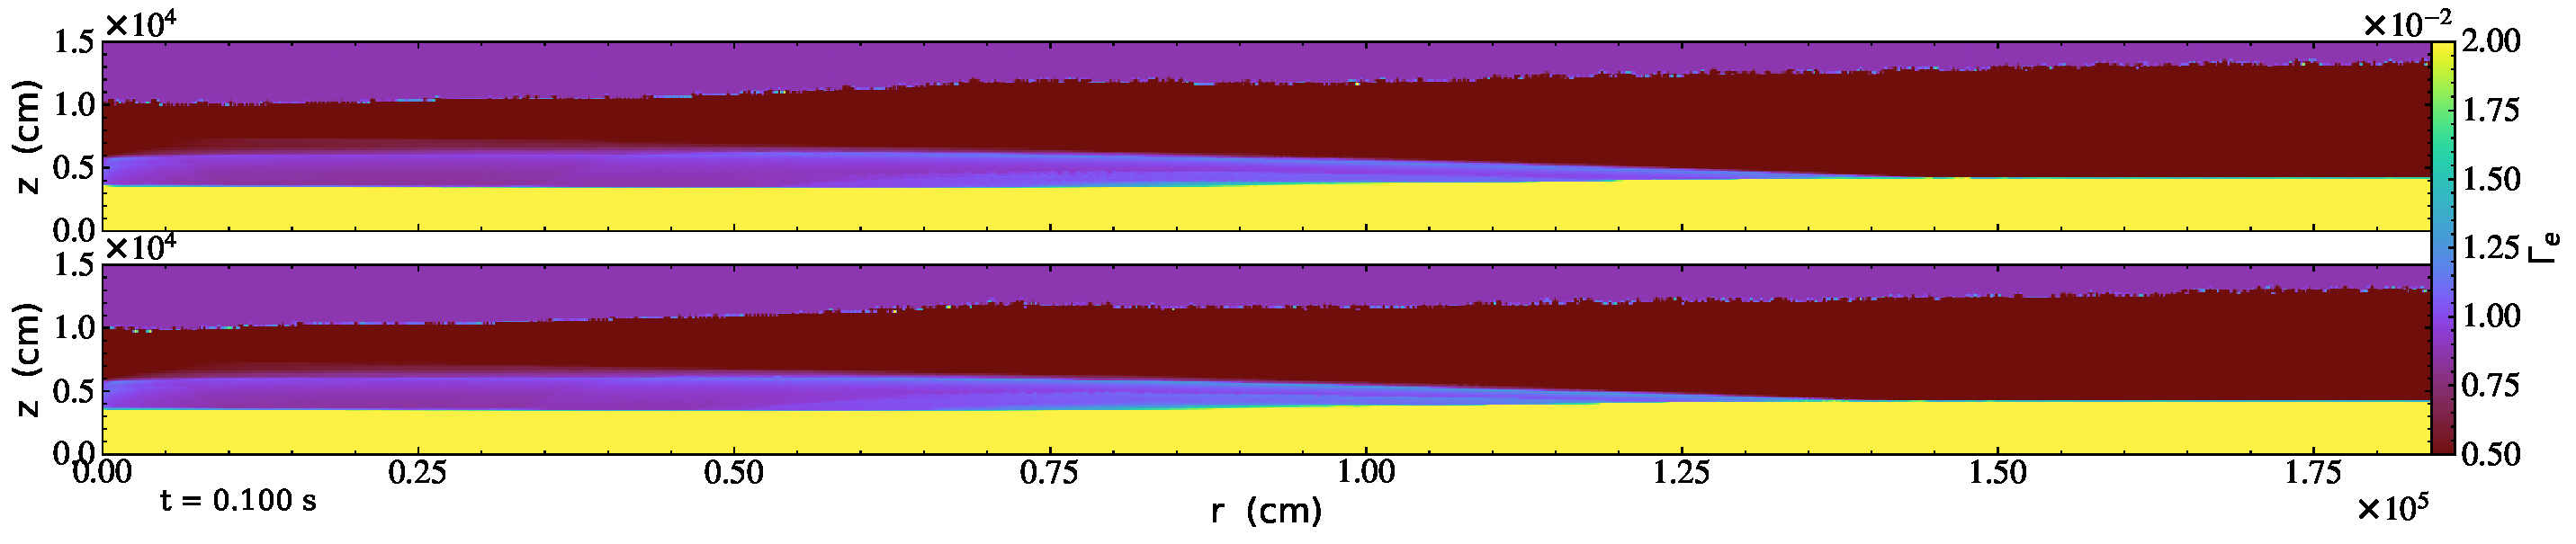
\includegraphics[width=1\linewidth]{screen_gamma_100ms.pdf}
%         \caption{\scriptsize {\it Top}: $\Gamma_e$ for {\tt aprox13}. {\it Bot}: $\Gamma_e$ for {\tt aprox13 chu}. Current time is $t = 100$ ms.}
%     \end{figure}

%     \column{0.25\linewidth}
%     \begin{block}{\scriptsize $\Gamma$ estimation}
%         \begin{itemize}
%             \item \scriptsize Triple-$\alpha$: $\Gamma \sim 0.05$ for $t = 50$ ms, $\Gamma \sim 0.025$ for $t = 100$ ms.
%             \item \scriptsize ${}^{16}$O + ${}^{16}$O:             $\Gamma \sim 0.48$ for $t = 50$ ms, $\Gamma \sim 0.32$ for $t = 100$ ms.
%         \end{itemize}
%     \end{block}
%     \end{columns}
% \end{frame}

% \begin{frame}{Screening: Weighted $T$ and $\dot{e}_{nuc}$ Time Profile}

%     \begin{figure}
%         \centering
%         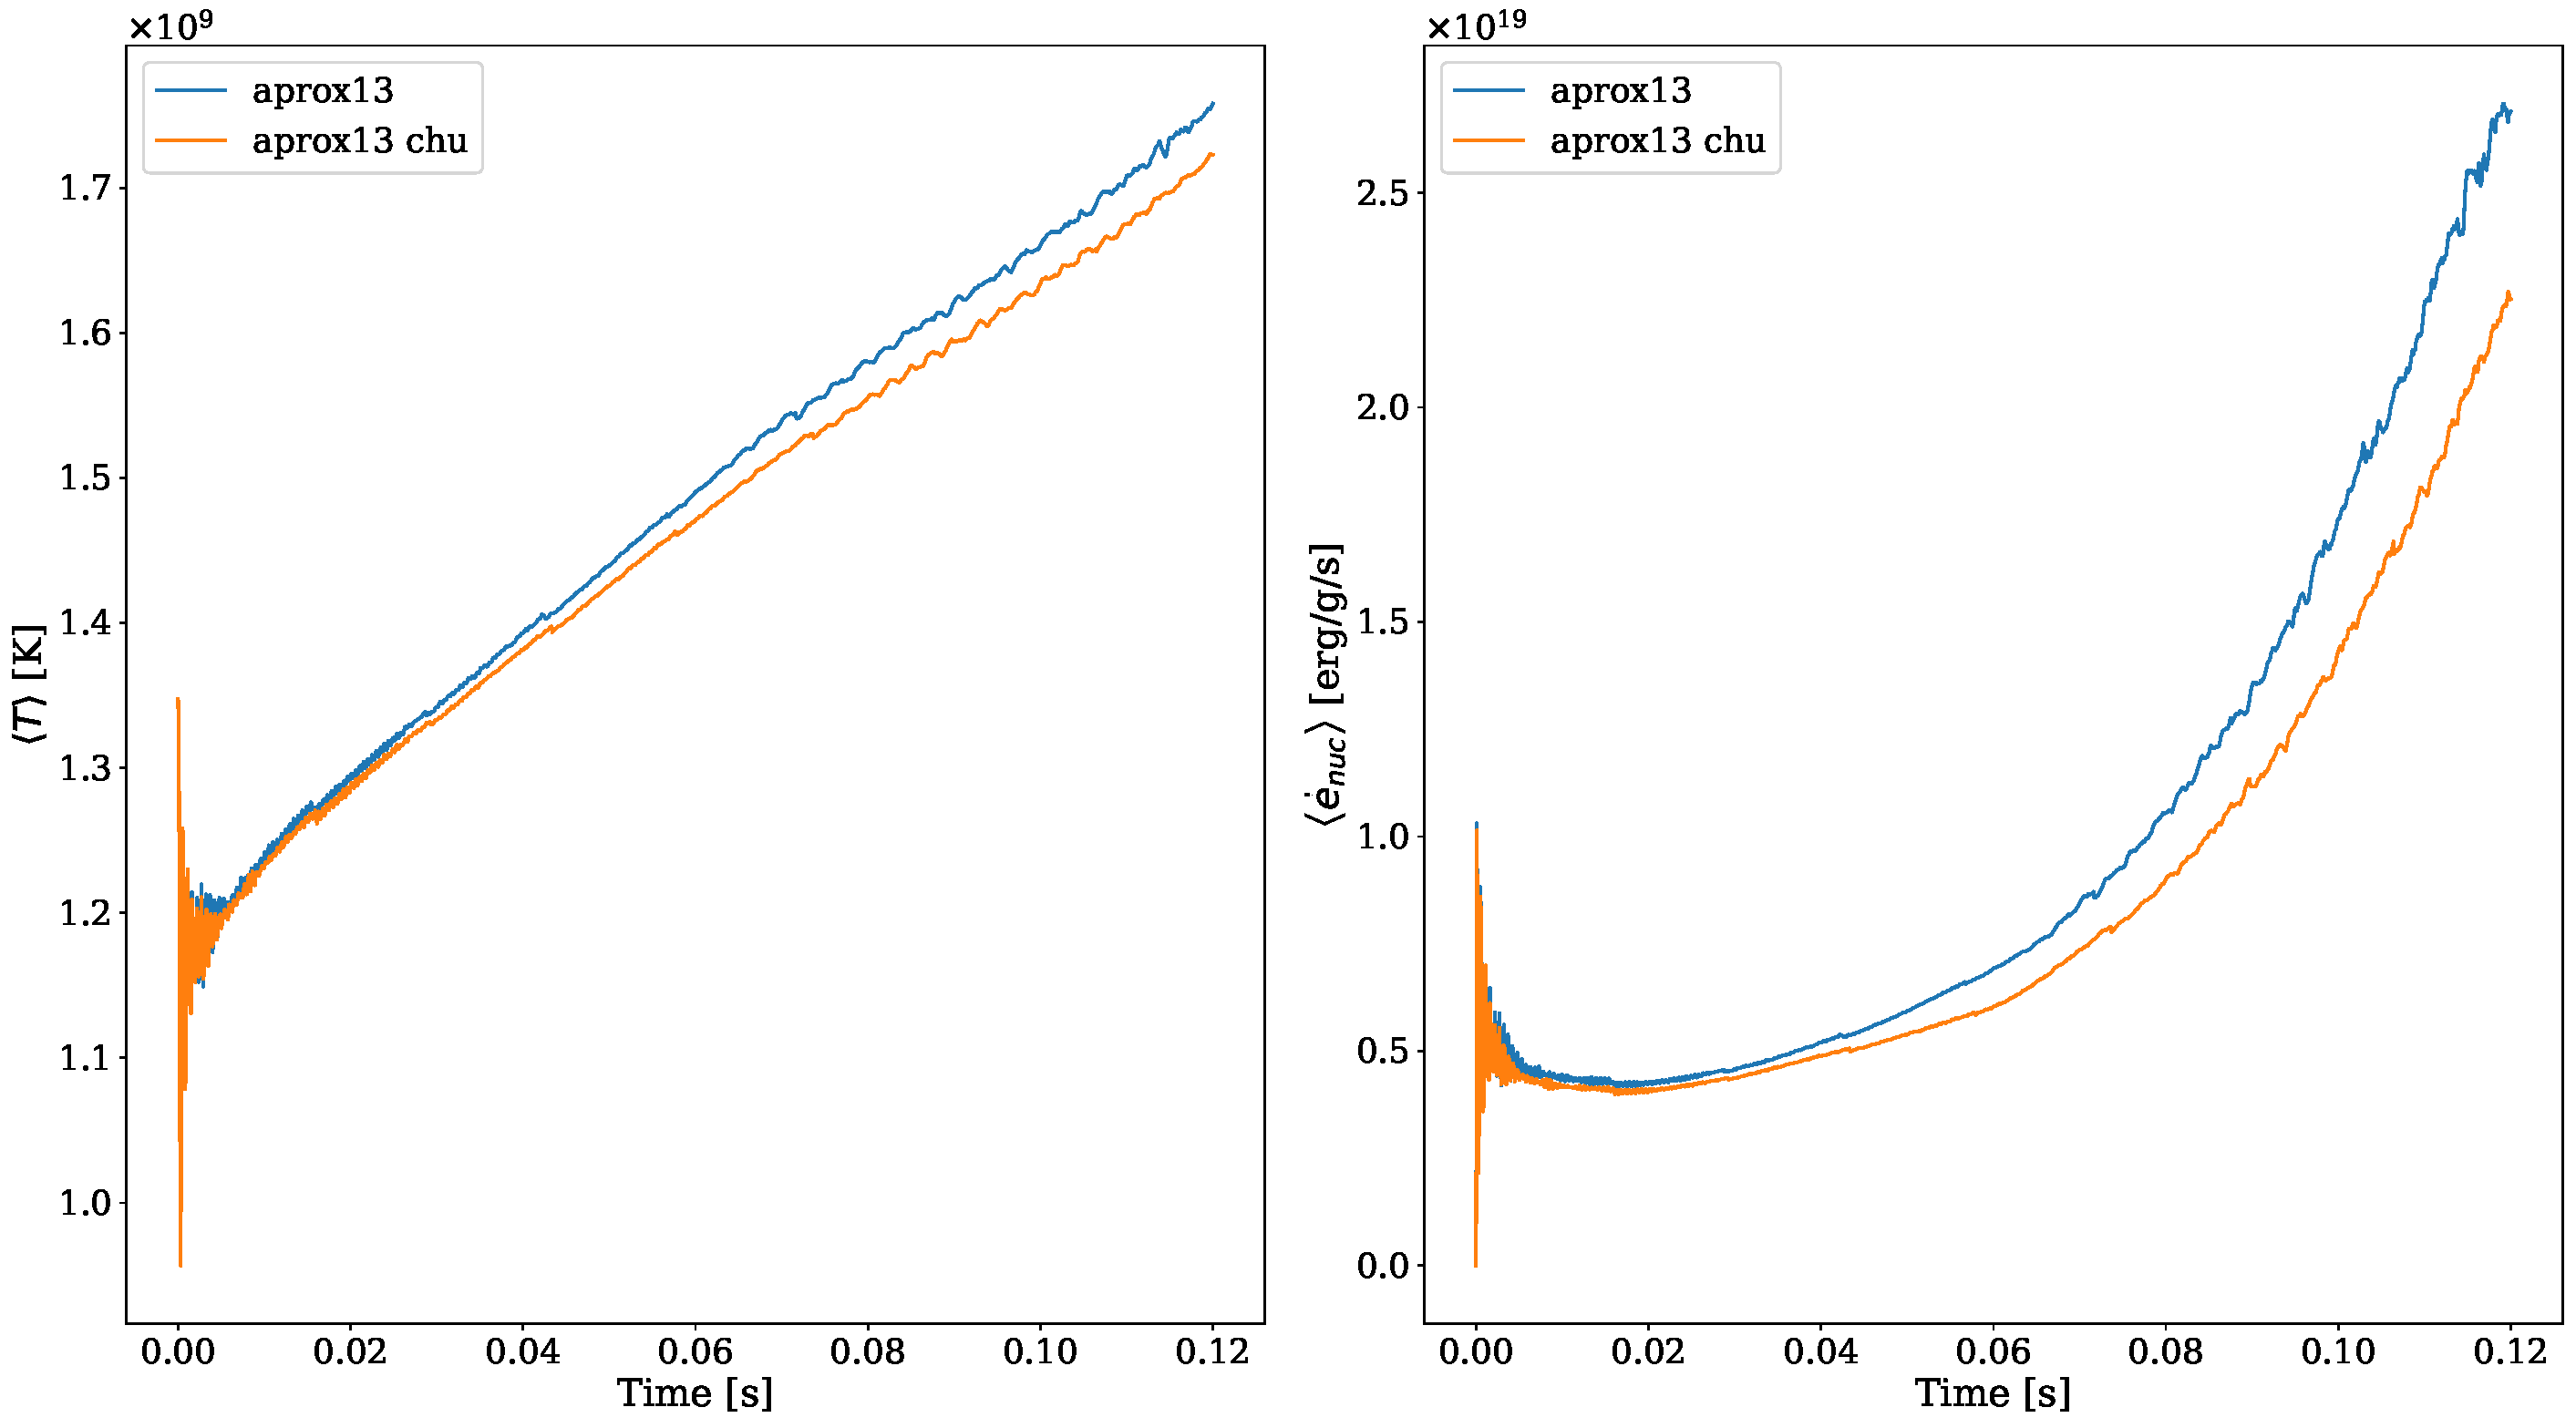
\includegraphics[width=1\linewidth]{screen_time_profile.pdf}
%         \caption{{\it Left}: Weighted temperature time profile. {\it Right}: Weighted specific nuclear energy generation rate time profile.}
%     \end{figure}
    
% \end{frame}


% \begin{frame}{Screening: Chugunov 2007 Comparison}
%     \begin{figure}
%         \centering
%         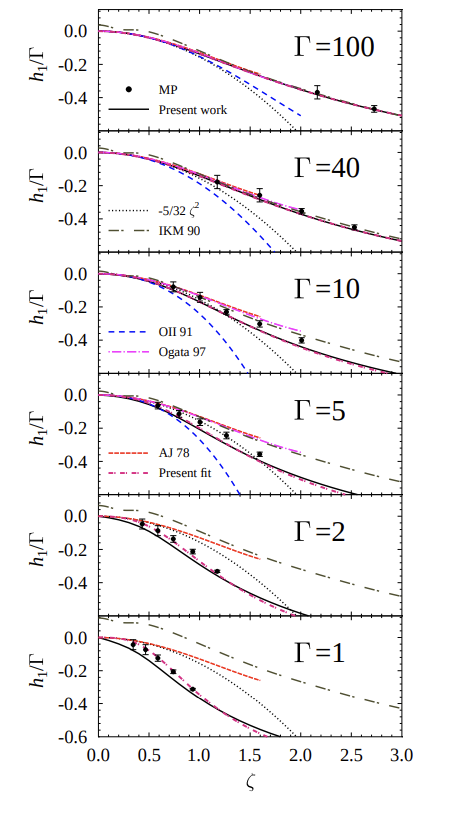
\includegraphics[width=0.33\linewidth]{chugunov2007.png}
%     \end{figure}

% \scriptsize Figure 4 in Chugunov 2007 \cite{Chugunov_2007}. The vertical axis represents the screening strength. The horizontal axis is a temperature parameter.
    
% \end{frame}



% \begin{frame}{Screening: Flame Front Position vs. Time}

%     \begin{figure}
%         \centering
%         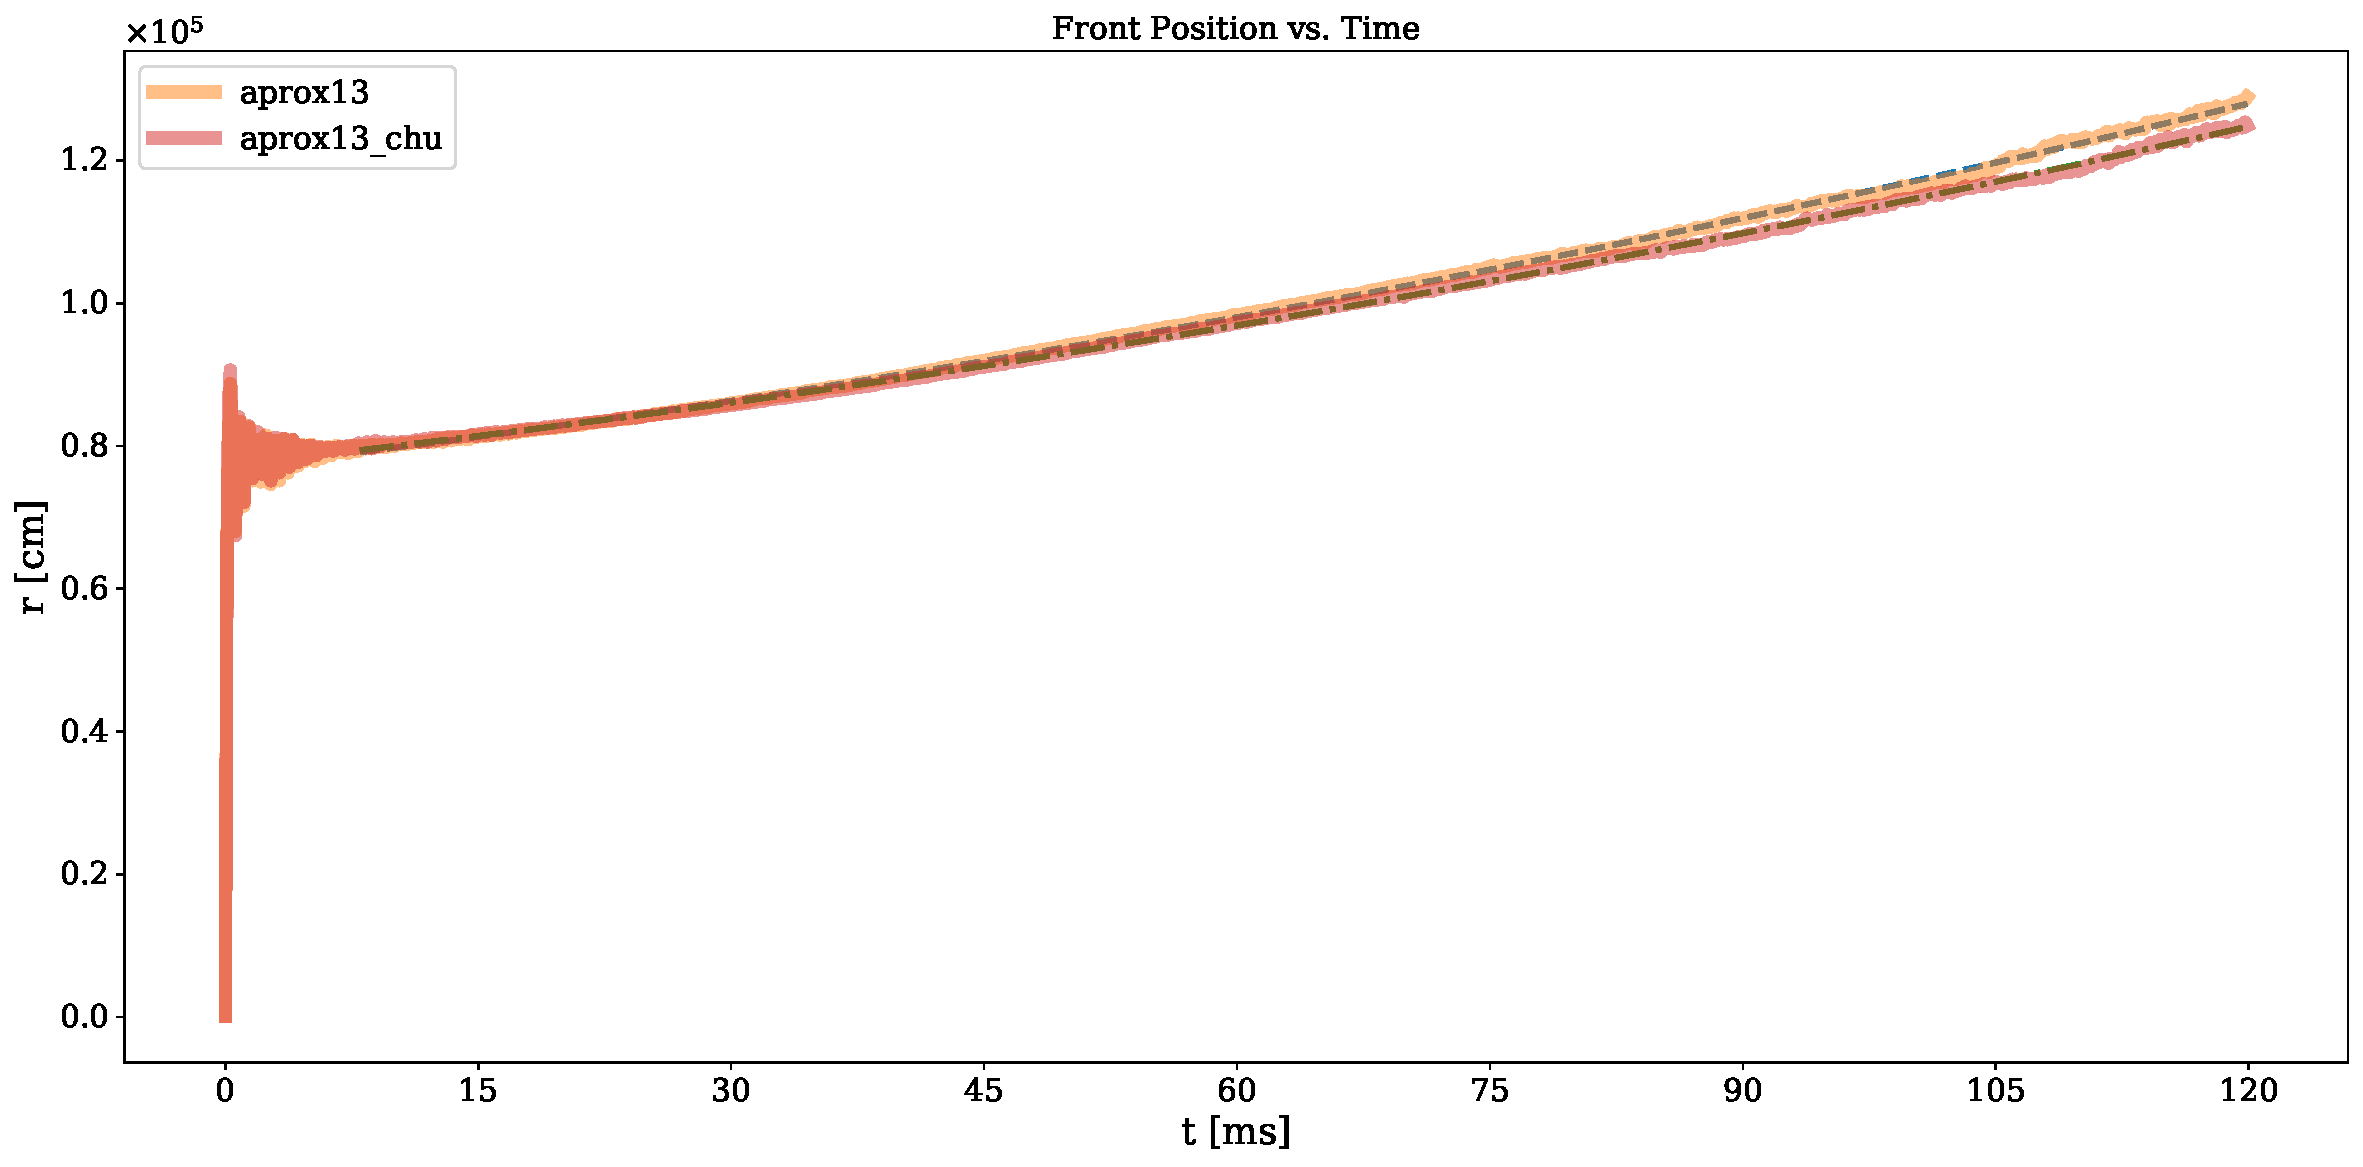
\includegraphics[width=1\linewidth]{screen_front.pdf}
%         \caption{This figure shows the flame front position as a function of time for {\tt aprox13} and {\tt aprox13 chu}.}
%     \end{figure}
% \end{frame}


% \begin{frame}[allowframebreaks]
% \frametitle{Screening: Flame Speed Comparison}

%     \begin{block}{Fitting Functions}
%         \begin{equation}
%             r(t) = \frac{1}{2}a_0 t^2 + v_0 t + r_0
%         \end{equation}
%     \end{block}
    
%     \begin{table}
%         \resizebox{1\linewidth}{!}{
%         \begin{tabular}{cccc}
%         \toprule
%         Name &
%         $a_0$ [$\mbox{km} \ \mbox{s}^{-2}$] &
%         $v_0$ [$\mbox{km} \ \mbox{s}^{-1}$] &
%         $r_0$ [km] \\
%         \midrule
%         {\tt aprox13} & $24.22 \pm 0.23$ & $2.812 \pm 0.015$ & $0.7680\pm 0.0004 $\\

%         {\tt aprox13 chu} & $22.96 \pm 0.20$ & $2.578 \pm 0.0133$ & $0.7728 \pm 0.0004$\\
%         \bottomrule
%         \end{tabular}}
%         \caption{This table shows the fitted parameters of the fitting functions. The fitting function is applied for $t > 8$ ms.}
%     \end{table}

%     \begin{table}
%         \resizebox{1\linewidth}{!}{
%         \begin{tabular}{cccc}
%         \toprule
%         Name &
%         $v_{23}$ [$\mbox{km} \ \mbox{s}^{-1}$] &
%         $v_{100}$ [$\mbox{km} \ \mbox{s}^{-1}$] &
%         $v_{120}$ [$\mbox{km} \ \mbox{s}^{-1}$] \\
%         \midrule
%         {\tt aprox13} & $3.369 \pm 0.016$ & $5.234 \pm 0.027$ & $5.718 \pm 0.031$\\
%         {\tt aprox13 chu} & $3.106 \pm 0.014$ & $4.874 \pm 0.024$ & $5.333 \pm 0.027$ \\
%         \bottomrule
%         \end{tabular}}
%         \caption{This table shows the instantaneous flame propagation speed at $t = 23$ ms, $t = 100$ ms and $t = 120$ ms. $t = 23$ ms represents the acceleration for {\tt subch full} and {\tt subch simple}. $t = 100$ ms and $t = 120$ ms represent the steady phase at the late-stage.}
%     \end{table}

% \end{frame}




% \section{Time Integration Methods}
% \subsection{Overview Time Integration Methods}


% \begin{frame}{Integration}
%     \begin{center}
%         \Huge {\it Effect of different time integration methods}
%     \end{center}
% \end{frame}

% % \begin{frame}{Introduction to Time Evolution Methods}
% %     \begin{block}
% %         Source terms for Euler's equation can be decomposed into hydrodynamic sources and reactive sources.
% %     \end{block}
% % \end{frame}

% \begin{frame}{strang-splitting vs. simplified-SDC}

%     \begin{block}{Strang-splitting}
%         \begin{itemize}
%             \item Consider hydrodynamics and nuclear reactions to be independent processes.
%             \item $\mathcal{U}^{n+1} = \mathcal{R}_{\Delta t/2} \mathcal{A}_{\Delta t} \mathcal{R}_{\Delta t/2} \mathcal{U}^n$
%             \item Indirect coupling between hydro-update and reaction.
%             \item Achieves second-order accuracy in time.

%         \end{itemize}
%     \end{block}
    
%     \begin{block}{simplified-SDC}
%         \begin{itemize}
%             \item Uses iterations (2) to construct higher-order accuracy solutions.
%             \item Direct Coupling between hydro-update and reaction.
%             \item Achieves second-order accuracy in time.
%         \end{itemize}
%     \end{block}

% \end{frame}

% \begin{frame}{Time Integration Methods: Models}

%     % \begin{center}
%     %     \LARGE Time Evolution Methods
%     % \end{center}
    
    
%     \begin{table}
%         \resizebox{1\linewidth}{!}{
%         \begin{tabular}{cccc}
%         \toprule
%         Name &
%         Network &
%         Integration &
%         Screening\\ 
%         \midrule
        
%         {\tt aprox13} & {\tt aprox13} & strang-splitting & {\tt SCREEN5} \\
%         {\tt subch full} & {\tt subch full} & strang-splitting & {\tt SCREEN5} \\
%         % {\tt subch full mod} & {\tt subch full mod} & strang-splitting & {\tt SCREEN5} \\
%         % {\tt subch simple} & {\tt subch simple} & strang-splitting & {\tt SCREEN5} \\
%         {\tt aprox13 sdc} & {\tt aprox13} & simplified SDC & {\tt SCREEN5} \\
%         {\tt subch full sdc} & {\tt subch full} & simplified SDC & {\tt SCREEN5} \\
%         % {\tt aprox13 chu} & {\tt aprox13} & strang-splitting & {\tt CHUGUNOV2007} \\
%         \bottomrule
%         \end{tabular}}
%         \caption{This table shows the various settings used for each simulation.}
%     \end{table}
    
% \end{frame}

% \subsection{Simulation Results}

% \begin{frame}{Integration: $\dot{e}_{nuc}$ Comparison}
%     \begin{figure}
%         \centering
%         \includegraphics[width=1\linewidth]{pres_integration_enuc_50ms.pdf}
%         \caption{{\it First (Top)}: $\dot{e}_{nuc}$ for {\tt aprox13}. {\it Second}: $\dot{e}_{nuc}$ for {\tt aprox13 sdc}. {\it Third}: $\dot{e}_{nuc}$ for {\tt subch full}. {\it Fourth (Bot)}: $\dot{e}_{nuc}$ for {\tt subch full sdc}.}
%     \end{figure}
% \end{frame}

% \begin{frame}{Integration: Weighted $T$ and $\dot{e}_{nuc}$ Time Profiles}
    
%     \begin{figure}
%         \centering
%         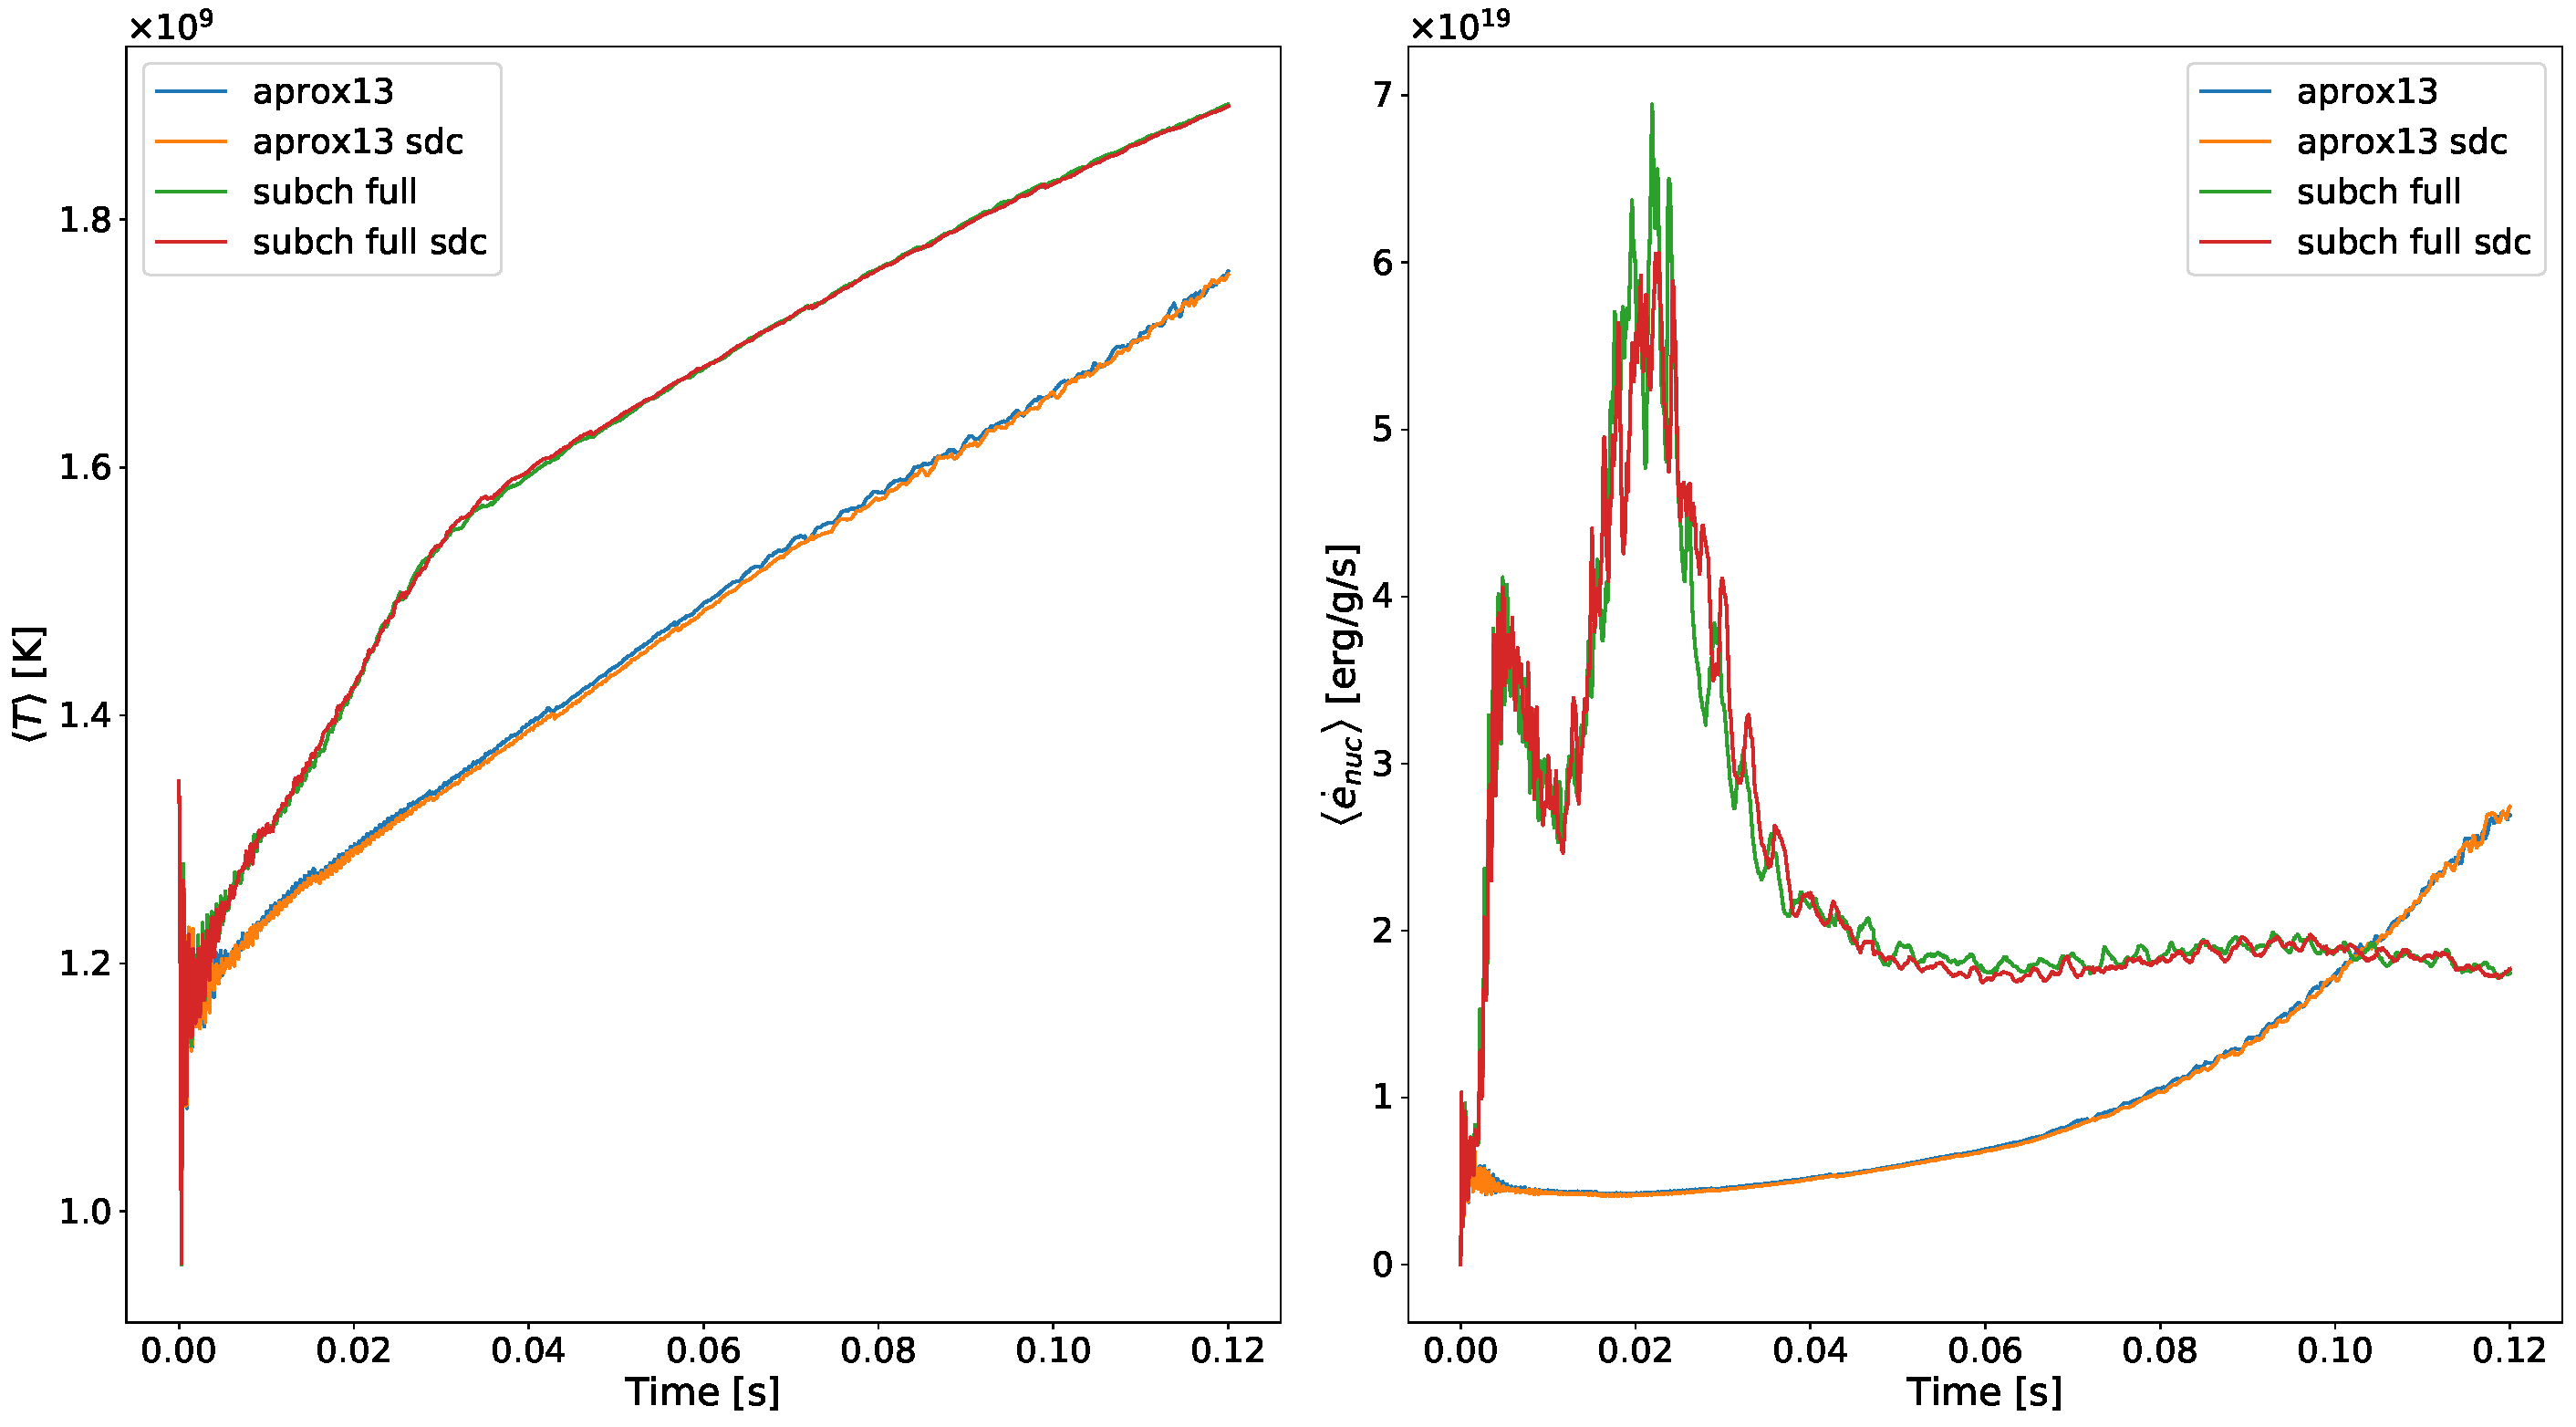
\includegraphics[width=0.95\linewidth]{integration_time_profile.pdf}
%         \caption{\scriptsize {\it Left}: weighted temperature for {\tt aprox13}, {\tt aprox13 sdc}, {\tt subch full}, and {\tt subch full sdc}. {\it Right}: specific energy generation rate for {\tt aprox13}, {\tt aprox13 sdc}, {\tt subch full}, and {\tt subch full sdc}.}
%     \end{figure}
% \end{frame}


% \begin{frame}{Integration: Front Position vs. Time}
    
%     \begin{figure}
%         \centering
%         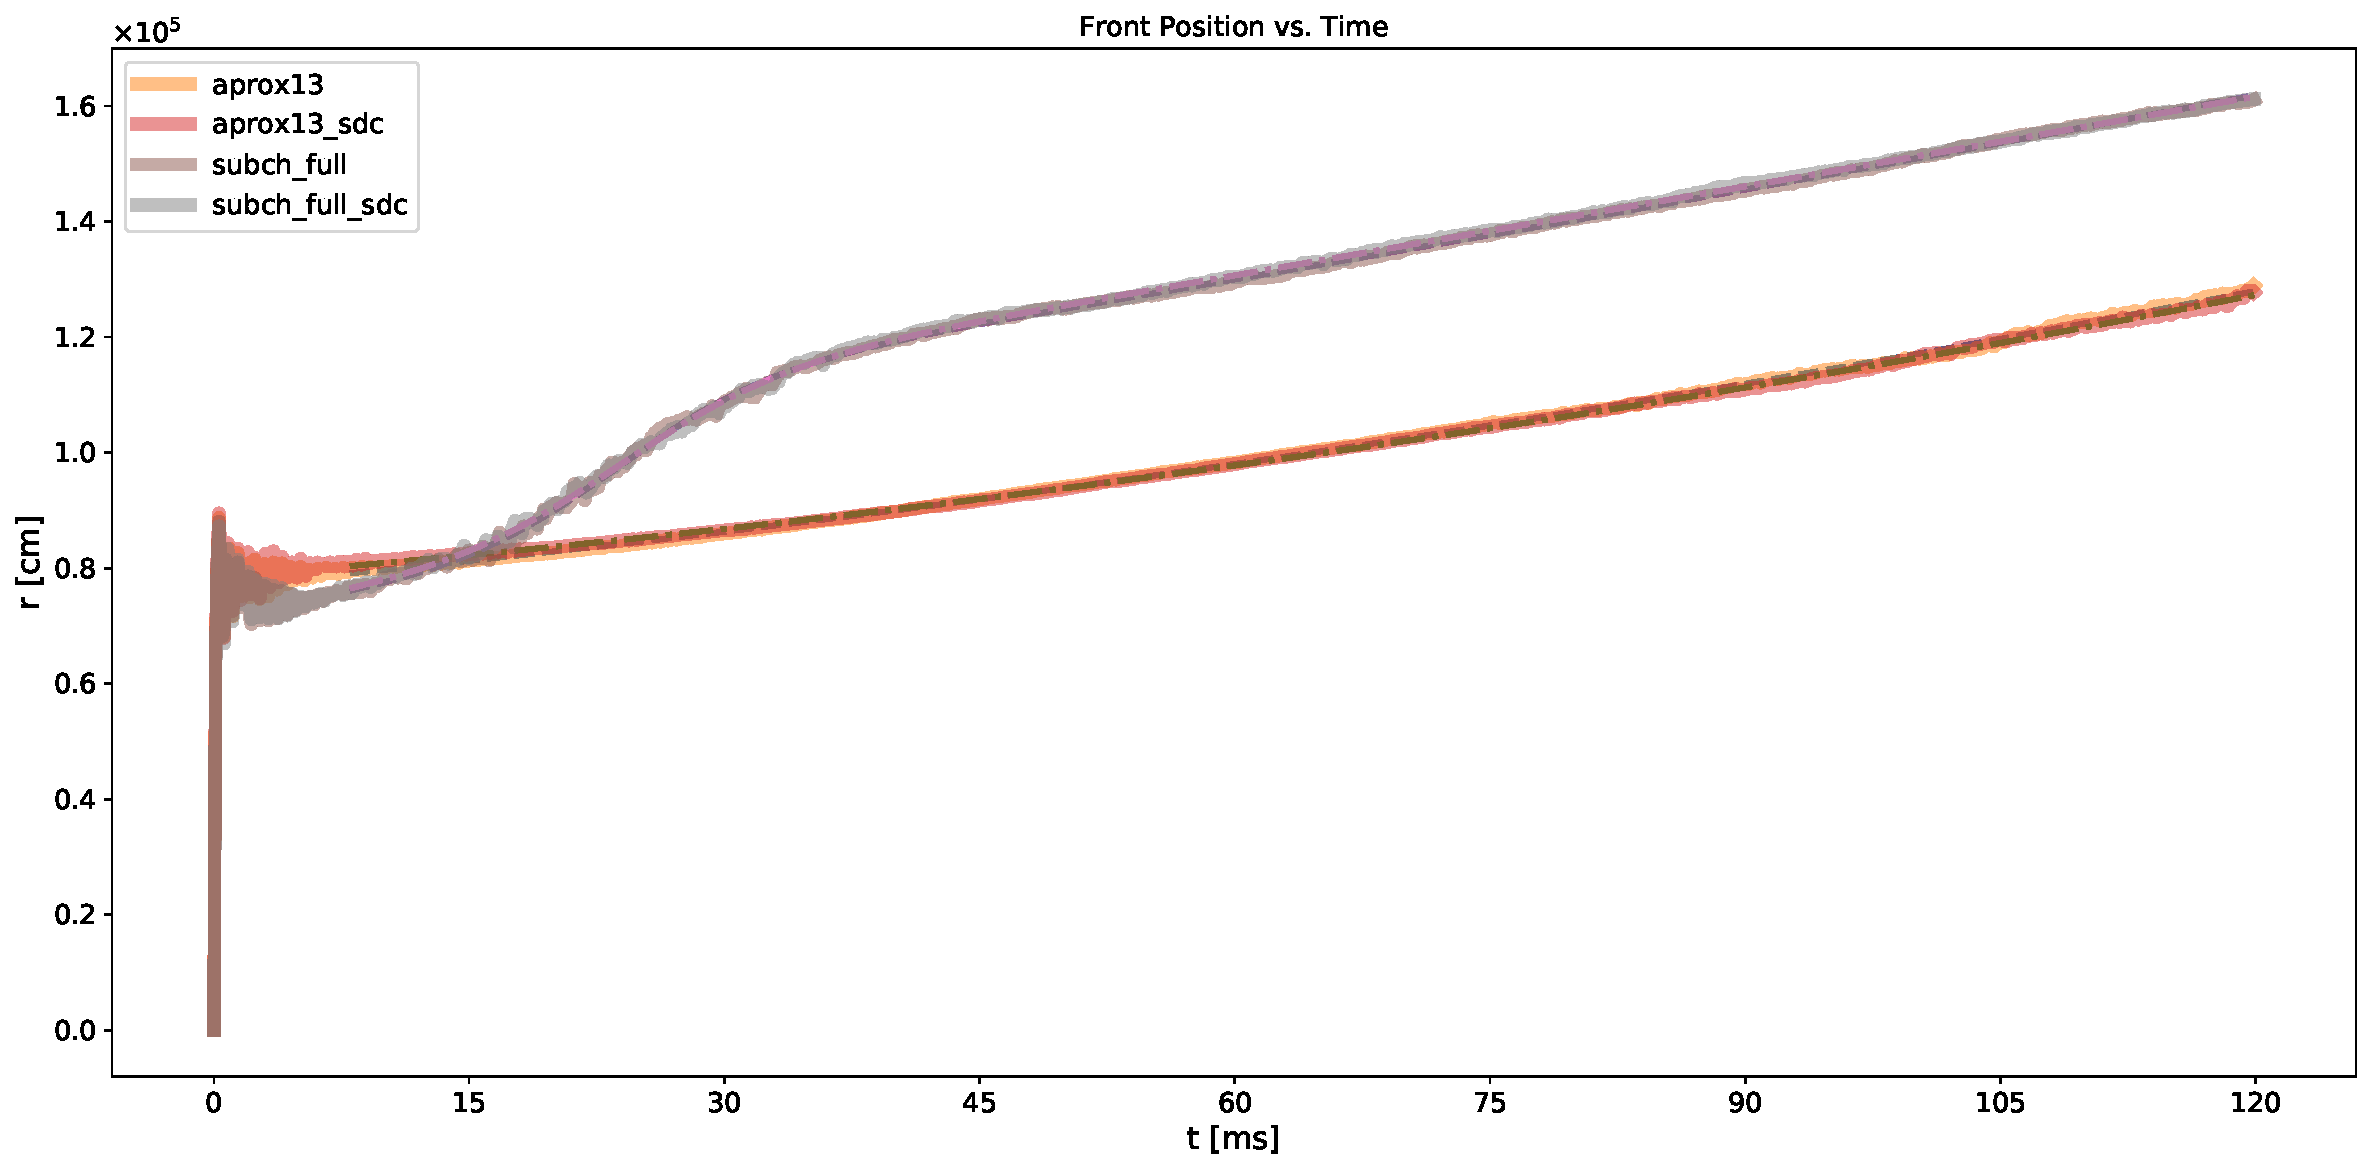
\includegraphics[width=1\linewidth]{integration_front.pdf}
%         \caption{Flame front position as a function of time for {\tt aprox13}, {\tt aprox13 sdc}, {\tt subch full}, and {\tt subch full sdc}. {\it Solid} Lines: Data. {\it Dashed} lines: fit.}
%     \end{figure}
% \end{frame}

% % \begin{frame}[allowframebreaks]
% % \frametitle{Integration: Flame Speed Comparison}
% %     \begin{block}{ Fitting Functions}
% %         \begin{subequations}
    
% %         \begin{equation}
% %              r(t) = \frac{1}{2}a_0 t^2 + v_0 t + r_0
% %         \end{equation}
        
% %         \begin{equation}
% %              r(t) = A\tanh{\left(\frac{t}{B} + C\right)} + \frac{1}{2}a_0 t^2 + v_0 t + r_0
% %         \end{equation}
% %         \end{subequations}
% %     \end{block}
    
% %     \begin{table}
% %         \resizebox{1\linewidth}{!}{
% %         \begin{tabular}{ccccccc}
% %         \toprule
% %         Name &
% %         $a_0$ [$\mbox{km} \ \mbox{s}^{-2}$] &
% %         $v_0$ [$\mbox{km} \ \mbox{s}^{-1}$] &
% %         $r_0$ [km] &
% %         A [$\mbox{km}$]&
% %         B [s]&
% %         C \\ 
% %         \midrule
% %         {\tt aprox13} & $24.22 \pm 0.23$ & $2.812 \pm 0.015$ & $0.7680\pm 0.0004 $ & N/A & N/A & N/A\\

% %         {\tt aprox13 sdc} & $28.09 \pm 0.20$ & $2.392 \pm 0.013$ & $0.7836\pm 0.0004 $ & N/A & N/A & N/A\\
        
% %         {\tt subch full} & $9.22 \pm 0.82$ & $4.489 \pm 0.067$ & $0.8646 \pm 0.0014$ & $0.150 \pm 0.001$ & $0.0093 \pm 0.0001$ & $-2.551 \pm 0.035$ \\
        
% %         {\tt subch full sdc} & $2.34 \pm 0.74$ & $4.947 \pm 0.061$ & $0.8601 \pm 0.0013$ & $0.146 \pm 0.001$ & $0.0098 \pm 0.0001$ & $-2.424 \pm 0.030$ \\
% %         \bottomrule
% %         \end{tabular}}
% %         \caption{\scriptsize This table shows the fitted parameters of the fitting functions. The fitting function is applied for $t > 8$ ms.}
% %     \end{table}

% %     \begin{table}
% %         \resizebox{1\linewidth}{!}{
% %         \begin{tabular}{cccc}
% %         \toprule
% %         Name &
% %         $v_{23}$ [$\mbox{km} \ \mbox{s}^{-1}$] &
% %         $v_{100}$ [$\mbox{km} \ \mbox{s}^{-1}$] &
% %         $v_{120}$ [$\mbox{km} \ \mbox{s}^{-1}$] \\
% %         \midrule
% %         {\tt aprox13} & $3.369 \pm 0.016$ & $5.234 \pm 0.027$ & $5.718 \pm 0.031$\\
% %         {\tt subch full} & $20.732 \pm 0.284$ & $5.411 \pm 0.105$ & $5.595 \pm 0.119$\\
% %         {\tt aprox13 sdc} & $3.039 \pm 0.014$ & $5.201 \pm 0.024$ & $5.764 \pm 0.027$\\
% %         {\tt subch full sdc} & $19.811 \pm 0.248$ & $5.181 \pm 0.096$ & $5.228 \pm 0.108$\\
% %         \bottomrule
% %         \end{tabular}}
% %         \caption{This table shows the instantaneous flame propagation speed at $t = 23$ ms, $t = 100$ ms and $t = 120$ ms. $t = 23$ ms represents the acceleration for {\tt subch full}, {\tt subch simple}, and {\tt subch full sdc}. $t = 100$ ms and $t = 120$ ms represent the steady phase at the late-stage.}
% %     \end{table}

% % \end{frame}

% \begin{frame}{Integration: $u-v$ Phase Plot}
%     \begin{figure}
%         \centering
%         \includegraphics[width=0.95\linewidth]{pres_integration_u_v_enuc_100ms.pdf}
%         \caption{\scriptsize {\it First (left)}: $u-v$ phase plot for {\tt aprox13}. {\it Second}: $u-v$ phase plot for {\tt aprox13 sdc}. {\it Third}: $u-v$ phase plot for {\tt subch full}. {\it Fourth (Right)}: $u-v$ phase plot for {\tt subch full sdc}. $t = 100$ ms}
%     \end{figure}
% \end{frame}

\section{Conclusion}

\begin{frame}
\frametitle{Conclusion}
    \begin{block}{Takeaways: Network Study}
    \begin{itemize}
        \item $(\alpha, \mbox{p})(\mbox{p}, \gamma)$ approximation continues to be an accurate approach in simulating thermonuclear flames propagations in XRBs. 
        
        \item The ${}^{12}\mbox{C}(\mbox{p}, \gamma) {}^{13}\mbox{N}(\alpha, \mbox{p}){}^{16}\mbox{O}$ rates are critical in accurately modelling flame propagation in XRBs. At $T \gtrsim 10^9$ K, these reactions dominate over the triple-$\alpha$ and the slow $\alpha$ capture processes from ${}^{12}$C to ${}^{16}$O. This allows an instant depletion of ${}^{12}$C, leading to a burst of energy and flame acceleration once temperature reaches $\sim 1.3 \times 10^9$ K.
    
        \item {\tt subch\_simple} network proved to be the most effective. It is the smallest network that captures the initial acceleration of the propagating flame, which drastically alters the overall flame dynamics.
    \end{itemize}
    \end{block}
    
%     % \begin{block}{Takeaways: Screening Study}
%     % \begin{itemize}
%     %     \item Thermonuclear flames in XRBs are likely in either weak or the intermediate screening regime.
%     %     \item {\tt SCREEN5} had a slightly stronger overall screening effect compared to {\tt CHUGUNOV2007}.
%     % \end{itemize}
%     % \end{block}
    
%     % \begin{block}{Takeaways: Integration Study}
%     % \begin{itemize}
%     %     \item strang-splitting and simplified-SDC had a similar overall performance.
%     %     \item Simplified-SDC had a stronger coupling between hydrodynamics and nuclear reactions. This is expected to be more significant at more extreme thermodynamic conditions.
%     %     % \item There is a minor computational artifact when plotting $\dot{e}_{nuc}$ for simplified-SDC.
%     % \end{itemize}
%     % \end{block}
\end{frame}


%------------------------------------------------
\begin{frame}
	\frametitle{Acknowledgements}
	
	\begin{columns}[t] % The "c" option specifies centered vertical alignment while the "t" option is used for top vertical alignment
		\begin{column}{0.45\textwidth} % Left column width
			\textbf{Current Group Members}
			\begin{itemize}
				\item Mike Zingale
				\item Eric Johnson
                    \item Alex Smith Clark
                    \item Khanak Bhargava

			\end{itemize}

                \textbf{Former Group Members}
                \begin{itemize}
                    \item Kiran Eiden
                    \item Max Katz
                    \item Alice Harpole
                    \item Donald Willcox
                \end{itemize}
		\end{column}
  
		\begin{column}{0.5\textwidth} % Right column width
			\textbf{Funding}
			\begin{itemize}
				\item The work at Stony Brook was supported by DOE/Office of Nuclear Physics grant DE-FG02-87ER40317.
				\item Supported by the Exascale Computing  Project (17-SC-20-SC)
				\item Used resources of the NERSC under Contract No.\ DE-AC02-05CH11231. 
				\item Used resources of the Oak Ridge Leadership Computing Facility under Contract No. DE-AC05-00OR22725.
			\end{itemize}
		\end{column}
	\end{columns}
\end{frame}


\begin{frame}[allowframebreaks]% Use [allowframebreaks] to allow automatic splitting across slides if the content is too long
	\frametitle{References}
    \printbibliography
\end{frame}

%----------------------------------------------------------------------------------------
%	ACKNOWLEDGMENTS SLIDE
%----------------------------------------------------------------------------------------


%----------------------------------------------------------------------------------------
%	CLOSING SLIDE
%----------------------------------------------------------------------------------------

\begin{frame}[plain] % The optional argument 'plain' hides the headline and footline
	\begin{center}
		{\Huge The End}
		
		\bigskip\bigskip % Vertical whitespace
		
		{\LARGE Questions? Comments?}
	\end{center}
\end{frame}

%----------------------------------------------------------------------------------------

% \begin{frame}
% \frametitle{Additional slide: Flame Speed Comparison}

%     \begin{block}{Fitting Functions}
%         \begin{subequations}
    
%         \begin{equation}
%              r(t) = \frac{1}{2}a_0 t^2 + v_0 t + r_0
%         \end{equation}
        
%         \begin{equation}
%              r(t) = A\tanh{\left(\frac{t}{B} + C\right)} + \frac{1}{2}a_0 t^2 + v_0 t + r_0
%         \end{equation}
%         \end{subequations}
%     \end{block}
    
%     \begin{table}
%         \resizebox{1\linewidth}{!}{
%         \begin{tabular}{ccccccc}
%         \toprule
%         Name &
%         $a_0$ [$\mbox{km} \ \mbox{s}^{-2}$] &
%         $v_0$ [$\mbox{km} \ \mbox{s}^{-1}$] &
%         $r_0$ [km] &
%         A [$\mbox{km}$]&
%         B [s]&
%         C \\ 
%         \midrule
%         {\tt aprox13} & $24.22 \pm 0.23$ & $2.812 \pm 0.015$ & $0.7680\pm 0.0004 $ & N/A & N/A & N/A\\
        
%         {\tt subch full} & $9.22 \pm 0.82$ & $4.489 \pm 0.067$ & $0.8646 \pm 0.0014$ & $0.150 \pm 0.001$ & $0.0093 \pm 0.0001$ & $-2.551 \pm 0.035$ \\
        
%         {\tt subch full mod} & $58.53 \pm 0.24$ & $2.122 \pm 0.016$ & $0.7773 \pm 0.0004$ & N/A & N/A & N/A \\
        
%         {\tt subch simple} & $15.60 \pm 0.93$ & $3.961 \pm 0.076$ & $0.8745 \pm 0.0016$ & $0.153 \pm 0.002$ & $0.0091 \pm 0.0001$ & $-2.575 \pm 0.040$\\
         
%         %{\tt aprox13 chu} & $22.96 \pm 0.20$ & $2.578 \pm 0.0133$ & $0.7728 \pm 0.0004$ & N/A & N/A & N/A\\
         
%         %{\tt aprox13 sdc} & $28.09 \pm 0.20$ & $2.392 \pm 0.013$ & $0.7836\pm 0.0004 $ & N/A & N/A & N/A\\
        
%         %{\tt subch full sdc} & $2.34 \pm 0.74$ & $4.947 \pm 0.061$ & $0.8601 \pm 0.0013$ & $0.146 \pm 0.001$ & $0.0098 \pm 0.0001$ & $-2.424 \pm 0.030$ \\
%         \bottomrule
%         \end{tabular}}
%         \caption{\scriptsize This table shows the fitted parameters of the fitting functions. The fitting function is applied for $t > 8$ ms.}
%     \end{table}
% \end{frame}

\end{document} 